\documentclass[10pt]{article}

\usepackage{../pplmanual} \NeedsTeXFormat{LaTeX2e}
\typeout{^^J^^J
Parallel Programming Laboratory^^J
Manual Style^^J
Written by Milind A. Bhandarkar, 12/00^^J}

%%% Make it possible for both ps and pdf to be generated
\newif\ifpdf
\ifx\pdfoutput\undefined
  \pdffalse
\else
  \pdfoutput=1
  \pdftrue
\fi

\ifpdf
  \pdfcompresslevel=9
\fi

%%% Imported from fullpage.sty, since it is not always available
\topmargin 0pt
\advance \topmargin by -\headheight
\advance \topmargin by -\headsep

\textheight 8.9in

\oddsidemargin 0pt
\evensidemargin \oddsidemargin
\marginparwidth 1.0in

\textwidth 6.5in
%%% end import from fullpage

%%% Commonly Needed packages
\usepackage{graphicx,color,calc}
\usepackage{makeidx}
\usepackage{alltt}

%%% Commands for uniform looks of C++, Charm++, and Projections
\newcommand{\CC}{C\kern -0.0em\raise 0.5ex\hbox{\normalsize++}}
\newcommand{\emCC}{C\kern -0.0em\raise 0.4ex\hbox{\normalsize\em++}}
\newcommand{\charmpp}{\sc Charm++}
\newcommand{\projections}{\sc Projections}
\newcommand{\converse}{\sc Converse}
\newcommand{\ampi}{\sc AMPI}

%%% Commands to produce margin symbols
\newcommand{\new}{\marginpar{\fbox{\bf$\mathcal{NEW}$}}}
\newcommand{\important}{\marginpar{\fbox{\bf\Huge !}}}
\newcommand{\experimental}{\marginpar{\fbox{\bf\Huge $\beta$}}}

%%% Commands for manual elements
\newcommand{\zap}[1]{ }
\newcommand{\function}[1]{{\noindent{\textsf{#1}}\\}}
\newcommand{\cmd}[1]{{\noindent{\textsf{#1}}\\}}
\newcommand{\args}[1]{\hspace*{2em}{\texttt{#1}}\\}
\newcommand{\param}[1]{{\texttt{#1}}}
\newcommand{\kw}[1]{{\textsf{#1}}}
\newcommand{\uw}[1]{{\textsl{#1}}}
\newcommand{\desc}[1]{\indent{#1}}

%%% Commands needed for Maketitle
\newcommand{\@version}{}
\newcommand{\@credits}{}
\newcommand{\version}[1]{\renewcommand{\@version}{#1}}
\newcommand{\credits}[1]{\renewcommand{\@credits}{#1}}

%%% Print the License Page
\newcommand{\@license}{%
 \begin{center}
   {University of Illinois}\\
   {\charmpp/\converse\ Parallel Programming System Software}\\
   {Non-Exclusive, Non-Commercial Use License}\\
 \end{center}
 \rule{\textwidth}{1pt}
{\tiny
Upon execution of this Agreement by the party identified below (``Licensee''),
The Board of Trustees of the University of Illinois  (``Illinois''), on behalf
of The Parallel Programming Laboratory (``PPL'') in the Department of Computer
Science, will provide the \charmpp/\converse\ Parallel Programming System
software (``\charmpp'') in Binary Code and/or Source Code form (``Software'')
to Licensee, subject to the following terms and conditions. For purposes of
this Agreement, Binary Code is the compiled code, which is ready to run on
Licensee's computer.  Source code consists of a set of files which contain the
actual program commands that are compiled to form the Binary Code.

\begin{enumerate}
  \item
    The Software is intellectual property owned by Illinois, and all right,
title and interest, including copyright, remain with Illinois.  Illinois
grants, and Licensee hereby accepts, a restricted, non-exclusive,
non-transferable license to use the Software for academic, research and
internal business purposes only, e.g. not for commercial use (see Clause 7
below), without a fee.

  \item 
    Licensee may, at its own expense, create and freely distribute
complimentary works that interoperate with the Software, directing others to
the PPL server (\texttt{http://charm.cs.uiuc.edu}) to license and obtain the
Software itself. Licensee may, at its own expense, modify the Software to make
derivative works.  Except as explicitly provided below, this License shall
apply to any derivative work as it does to the original Software distributed by
Illinois.  Any derivative work should be clearly marked and renamed to notify
users that it is a modified version and not the original Software distributed
by Illinois.  Licensee agrees to reproduce the copyright notice and other
proprietary markings on any derivative work and to include in the documentation
of such work the acknowledgement:

\begin{quote}
``This software includes code developed by the Parallel Programming Laboratory
in the Department of Computer Science at the University of Illinois at
Urbana-Champaign.''
\end{quote}

Licensee may redistribute without restriction works with up to 1/2 of their
non-comment source code derived from at most 1/10 of the non-comment source
code developed by Illinois and contained in the Software, provided that the
above directions for notice and acknowledgement are observed.  Any other
distribution of the Software or any derivative work requires a separate license
with Illinois.  Licensee may contact Illinois (\texttt{kale@cs.uiuc.edu}) to
negotiate an appropriate license for such distribution.

  \item
    Except as expressly set forth in this Agreement, THIS SOFTWARE IS PROVIDED
``AS IS'' AND ILLINOIS MAKES NO REPRESENTATIONS AND EXTENDS NO WARRANTIES OF
ANY KIND, EITHER EXPRESS OR IMPLIED, INCLUDING BUT NOT LIMITED TO WARRANTIES OR
MERCHANTABILITY OR FITNESS FOR A PARTICULAR PURPOSE, OR THAT THE USE OF THE
SOFTWARE WILL NOT INFRINGE ANY PATENT, TRADEMARK, OR OTHER RIGHTS.  LICENSEE
ASSUMES THE ENTIRE RISK AS TO THE RESULTS AND PERFORMANCE OF THE SOFTWARE
AND/OR ASSOCIATED MATERIALS.  LICENSEE AGREES THAT UNIVERSITY SHALL NOT BE HELD
LIABLE FOR ANY DIRECT, INDIRECT, CONSEQUENTIAL, OR INCIDENTAL DAMAGES WITH
RESPECT TO ANY CLAIM BY LICENSEE OR ANY THIRD PARTY ON ACCOUNT OF OR ARISING
FROM THIS AGREEMENT OR USE OF THE SOFTWARE AND/OR ASSOCIATED MATERIALS.

  \item 
    Licensee understands the Software is proprietary to Illinois. Licensee
agrees to take all reasonable steps to insure that the Software is  protected
and secured from unauthorized disclosure, use, or release and  will treat it
with at least the same level of care as Licensee would use to  protect and
secure its own proprietary computer programs and/or information, but using no
less than a reasonable standard of care.  Licensee agrees to provide the
Software only to any other person or entity who has registered with Illinois.
If licensee is not registering as an individual but as an institution or
corporation each member of the institution or corporation who has access to or
uses Software must agree to and abide by the terms of this license. If Licensee
becomes aware of any unauthorized licensing, copying or use of the Software,
Licensee shall promptly notify Illinois in writing. Licensee expressly agrees
to use the Software only in the manner and for the specific uses authorized in
this Agreement.

  \item
    By using or copying this Software, Licensee agrees to abide by the
copyright law and all other applicable laws of the U.S. including, but not
limited to, export control laws and the terms of this license. Illinois  shall
have the right to terminate this license immediately by written  notice upon
Licensee's breach of, or non-compliance with, any terms of the license.
Licensee may be held legally responsible for any  copyright infringement that
is caused or encouraged by its failure to  abide by the terms of this license.
Upon termination, Licensee agrees to  destroy all copies of the Software in its
possession and to verify such  destruction in writing.

  \item
  The user agrees that any reports or published results obtained with  the
Software will acknowledge its use by the appropriate citation as  follows:

\begin{quote}
``\charmpp/\converse\ was developed by the Parallel Programming Laboratory in
the Department of Computer Science at the University of  Illinois at
Urbana-Champaign.''
\end{quote}

Any published work which utilizes \charmpp\ shall include the following
reference:

\begin{quote}
``L. V. Kale and S. Krishnan. \charmpp: Parallel Programming with Message-Driven
Objects. In 'Parallel Programming using \CC' (Eds. Gregory V. Wilson and Paul
Lu), pp 175-213, MIT Press, 1996.''
\end{quote}

Any published work which utilizes \converse\ shall include the following
reference:

\begin{quote}
``L. V. Kale, Milind Bhandarkar, Narain Jagathesan, Sanjeev Krishnan and Joshua
Yelon. \converse: An Interoperable Framework for Parallel Programming.
Proceedings of the 10th International Parallel Processing Symposium, pp
212-217, April 1996.''
\end{quote}

Electronic documents will include a direct link to the official \charmpp\ page
at \texttt{http://charm.cs.uiuc.edu/}

  \item
    Commercial use of the Software, or derivative works based thereon,
REQUIRES A COMMERCIAL LICENSE.  Should Licensee wish to make commercial use of
the Software, Licensee will contact Illinois (kale@cs.uiuc.edu) to negotiate an
appropriate license for such use. Commercial use includes: 

    \begin{enumerate}
      \item
	integration of all or part of the Software into a product for sale,
lease or license by or on behalf of Licensee to third parties, or 

      \item
	distribution of the Software to third parties that need it to
commercialize product sold or licensed by or on behalf of Licensee.
    \end{enumerate}

  \item
    Government Rights. Because substantial governmental funds have been  used
in the development of \charmpp/\converse, any possession, use or sublicense of
the Software by or to the United States government shall be subject to such
required restrictions.

  \item
    \charmpp/\converse\ is being distributed as a research and teaching tool
and as such, PPL encourages contributions from users of the code that might, at
Illinois' sole discretion, be used or incorporated to make the basic  operating
framework of the Software a more stable, flexible, and/or useful  product.
Licensees who contribute their code to become an internal  portion of the
Software agree that such code may be distributed by  Illinois under the terms
of this License and may be required to sign an  ``Agreement Regarding
Contributory Code for \charmpp/\converse\ Software'' before Illinois  can
accept it (contact \texttt{kale@cs.uiuc.edu} for a copy).
\end{enumerate}

UNDERSTOOD AND AGREED.

Contact Information:

The best contact path for licensing issues is by e-mail to
\texttt{kale@cs.uiuc.edu} or send correspondence to:

\begin{quote}
Prof. L. V. Kale\\
Dept. of Computer Science\\
University of Illinois\\
1304 W. Springfield Ave\\
Urbana, Illinois 61801 USA\\
FAX: (217) 333-3501
\end{quote}
}%tiny
 \newpage
}% end of license

\renewcommand{\maketitle}{\begin{titlepage}%
 \begin{flushright}
   {\Large
     Parallel Programming Laboratory\\
     University of Illinois at Urbana-Champaign\\
   }
 \end{flushright}
 \rule{\textwidth}{3pt}
 \vspace{\fill}
 \begin{flushright}
   \textsf{\Huge \@title \\}
 \end{flushright}
 \vspace{\fill}
 \@credits \\
 \rule{\textwidth}{3pt}
 \begin{flushright}
   {\large Version \@version}
 \end{flushright}
 \end{titlepage}
 \@license

 \tableofcontents
 \newpage
}% maketitle

 \usepackage{html}
\title{The\\ \charmpp\\ Programming Language\\ Manual} \version{6.0
  (Release 1)} \credits{ {\small The Charm software was developed as a
    group effort.  The earliest prototype, Chare Kernel(1.0), was
    developed by Wennie Shu and Kevin Nomura working with Laxmikant
    Kale.  The second prototype, Chare Kernel(2.0), a complete
    re-write with major design changes, was developed by a team
    consisting of Wayne Fenton, Balkrishna Ramkumar, Vikram Saletore,
    Amitabh B. Sinha and Laxmikant Kale. The translator for Chare
    Kernel(2.0) was written by Manish Gupta.  Charm(3.0), with
    significant design changes, was developed by a team consisting of
    Attila Gursoy, Balkrishna Ramkumar, Amitabh B.  Sinha and
    Laxmikant Kale, with a new translator written by Nimish Shah.  The
    \charmpp\ implementation was done by Sanjeev Krishnan.  Charm(4.0)
    included \charmpp\ and was released in fall 1993.  Charm(4.5) was
    developed by Attila Gursoy, Sanjeev Krishnan, Milind Bhandarkar,
    Joshua Yelon, Narain Jagathesan and Laxmikant Kale.  Charm(4.8),
    developed by the same team included Converse, a parallel runtime
    system that allows interoperability among modules written using
    different paradigms within a single application. \charmpp\ runtime
    system was re-targetted at Converse. Syntactic extensions in
    \charmpp\ were dropped, and a simple interface translator was
    developed (by Sanjeev Krishnan and Jay DeSouza) that, along with
    the \charmpp\ runtime, became the \charmpp\ language.  Charm
    (5.4R1) included the following: a complete rewrite of the
    \charmpp\ runtime system (using \CC) and the interface translator
    (done by Milind Bhandarkar), several new features such as Chare
    Arrays (developed by Robert Brunner and Orion Lawlor), various
    libraries (written by Terry Wilmarth, Gengbin Zheng, Laxmikant
    Kale, Zehra Sura, Milind Bhandarkar, Robert Brunner, and Krishnan
    Varadarajan.) A coordination language ``Structured Dagger'' was
    been implemented on top of \charmpp\ (Milind Bhandarkar), dynamic
    seed-based load balancing (Terry Wilmarth and Joshua Yelon), a
    client-server interface for Converse programs, and debugging
    support by Parthasarathy Ramachandran, Jeff Wright, and Milind
    Bhandarkar, Projections, the performance visualization and
    analysis tool, was redesigned and rewritten using Java by Michael
    Denardo. The test suite for \charmpp\ was developed by Michael
    Lang, Jackie Wang, and Fang Hu. Converse was been ported to ASCI
    Red (Joshua Yelon), Cray T3E (Robert Brunner), and SGI Origin2000
    (Milind Bhandarkar). For the current version Charm 6.0 (R1),
    Converse has been ported to new platforms including BlueGene/[LP]
    (Kumar, Huang, Bhatele), Cray XT3/4 (Zheng), Apple G5, Myrinet
    (Zheng), and Infiniband (Chakravorty).  Charm 6.0 introduces a
    dedicated no network SMP multicore Converse layer for stand-alone
    workstation experimenters (Zheng, Chakravorty, Kale, Jetley).
    Charm 6.0 also includes cross platform network topology aware
    chare placement for 3D tori and mesh networks (Kumar, Huang,
    Bhatele, Bohm). The test suite was extended for automated testing
    on all supported platforms by Gengbin Zheng.  The Projection tool
    was substantially improved by Chee Wai Lee and Isaac Dooley. The
    Control Point performance tuning framework was created by Isaac
    Dooley. Debugging support was enhanced with memory inspection
    features by Filippo Gioachin. The Charisma orchestration language
    was implemented on top of Charm++ by Chao Huang and Sanjay Kale.
    Sanjay Kale, Orion Lawlor, Gengbin Zheng, Terry Wilmarth, Filippo
    Gioachin, Sayantan Chakravorty, Chao Huang, David Kunzman, Isaac
    Dooley, Eric Bohm, Sameer Kumar, Chao Mei, Pritish Jetley, and
    Abhinav Bhatele, have been responsible for the changes to the
    system since the last release.  } }

\begin{document}

\maketitle

This manual describes \charmpp\ and Converse libraries.\cite{InterOpIPPS96}
This is a work in progress towards a standard library for parallel
programming on top of the Converse and \charmpp\ system.

For a description of the C-based {\sc Charm} parallel programming system,
please refer to the {\sl Charm Programming Language Manual} and the
{\sl Tutorial Introduction to Charm}\footnote{{\sc Charm} is no longer
actively supported and maintained, and these manuals are kept only for
offering the historical perspectives.}.


\section{Big Questions}

\subsubsection{What is Charm++?}

\htmladdnormallink{Charm++}{http://charm.cs.uiuc.edu/research/charm/} is
a runtime library to let C++ objects communicate with each other efficiently.
The programming model is thus very much like CORBA, Java RMI, or RPC; but
it is targeted towards tightly coupled, high-performance parallel machines.
It uses the ``single program, multiple data'' (SPMD) programming model made
popular by MPI.

Charm++ has demonstrated scalability up to thousands of processors,
and provides extremely advanced load balancing and object migration facilities.

\subsubsection{Can Charm++ parallelize my serial program automatically?}

No.

Charm++ is used to write ``explicitly parallel'' programs--we don't have
our own compiler, so we don't do automatic parallelization. We've found
automatic parallelization useful only for a small range of very regular
numerical applications.

However, you should { \em not} have to throw away your serial code;
normally only a small fraction of a large program needs to be changed to
enable parallel execution. In particular, Charm++'s support for object-oriented
programming and high-level abstractions such as Charm++ Arrays make it
simpler and more expressive than many other parallel languages. So you
will have to write some new code, but not as much as you might think. This
is particularly true when using one of the Charm++ \htmladdnormallink{frameworks}{http://charm.cs.uiuc.edu/research/}.

\subsubsection{I can already write parallel applications in MPI. Why should I use Charm++?}

Charm++ provides several extremely sophisticated features, such as
application-independent object migration, that are very difficult to provide
in MPI. If you have a working MPI code but have scalability problems
because of dynamic behavior, load imbalance, or communication costs, Charm++
might dramatically improve your performance. You can even run your
MPI code on Charm++ unchanged using \htmladdnormallink{AMPI}{http://charm.cs.uiuc.edu/research/ampi/}.

\subsubsection{Will Charm++ run on my machine?}

Yes.

Charm++ supports both shared-memory and distributed-memory machines,
SMPs and non-SMPs. In particular, we support serial machines, Windows
machines, clusters connected via Ethernet, Myrinet or Infiniband, IBM
SP series and BlueGene, Cray XT series, and any machine that supports MPI
or SHMEM. We normally do our development on Linux workstations, and
our testing on large parallel machines. Programs written using Charm++
will run on any supported machine.

No one has ported Charm++ to a vector supercomputer, but it should be
possible.

\subsubsection{Does anybody actually use Charm++?}

Yes.

The large, production-quality molecular dynamics application \htmladdnormallink{NAMD}{http://charm.cs.uiuc.edu/research/moldyn/}
is built on Charm++.\\
The \htmladdnormallink{Center for Simulation of Advanced Rockets}{http://www.csar.uiuc.edu/}
has a large physical simulation code built using Charm++.\\
We have significant collaborations with groups in Materials Science,
Chemistry, and Astrophysics in Illinios, New York, and Washington.

\subsubsection{Who created Charm++?}

Prof. \htmladdnormallink{L.V. Kale}{mailto:kale@cs.uiuc.edu}, of the
\htmladdnormallink{Computer Science Department}{http://www.cs.uiuc.edu/}
of the \htmladdnormallink{University of Illinois at Urbana-Champaign}{http://www.uiuc.edu/},
and his research group, the \htmladdnormallink{Parallel Programming Lab}{http://charm.cs.uiuc.edu/">Parallel}.
Nearly a hundred people have contributed something
to the project over the course of aproximately 15 years; a partial list
of contributors appears in the \htmladdnormallink{people}{http://charm.cs.uiuc.edu/people/}'s page.

\subsubsection{What is the future of Charm++?}

Our research group of approximately twenty people are actively engaged
in maintaining and extending Charm++; and in particular the Charm++ 
\htmladdnormallink{frameworks}{http://charm.cs.uiuc.edu/research/}.
Several other groups are dependent on Charm++, so we expect to continue
improving Charm++ indefinitely.

\subsubsection{How is Charm++ Licensed?}

Charm++ is open-source and free for research, educational, and academic
use. The University of Illinois retains the copyright to the software,
and requires a license for any commercial redistribution of our software.
The actual, legal license is included with Charm++ (in charm/LICENSE).

\subsubsection{I have a suggestion/feature request/bug report. Who should I send
it to?}

Our mailing list is \htmladdnormallink{ppl@cs.uiuc.edu}{mailto:ppl@cs.uiuc.edu}.
We're always glad to get feedback on our software.


\section{The \charmpp\ Language}
  \subsection{Modules}

\subsubsection{Structure of a \charmpp\ Program}

A \charmpp\ program is structurally similar to a \CC{} program.  Most of a
\charmpp\ program {\em is} \CC{} code \footnote{\bf Constraint: The \CC{} code
cannot, however, contain global or static variables.}. The main syntactic units
in a \charmpp\ program are class definitions. A \charmpp\ program can be
distributed across several source code files.

There are five disjoint categories of objects (classes) in \charmpp:

\begin{itemize}
\item Sequential objects: as in \CC{}
\item Chares (concurrent objects) \index{chare}
\item Chare Groups \index{chare groups} (a form of replicated objects)
\index{group}
\item Chare Arrays \index{chare arrays} (an indexed collection of chares)
\index{array}
\item Messages (communication objects)\index{message}
\end{itemize}

The user's code is written in \CC{} and interfaces with the \charmpp\ system as
if it were a library containing base classes, functions, etc.  A translator is
used to generate the special code needed to handle \charmpp\ constructs.  This
translator generates \CC{} code that needs to be compiled with the user's code.

Interfaces to the \charmpp\ objects (such as messages, chares, readonly
variables etc.) \index{message}\index{chare}\index{readonly} have to be
declared in \charmpp\ interface files. Typically, such entities are grouped
\index{module} into {\em modules}. A \charmpp\ program may consists of multiple
modules.  One of these modules is declared to be a \kw{mainmodule}. All the
modules that are ``reachable'' from the \kw{mainmodule} via the \kw{extern}
construct are included in a \charmpp\ program.

The \charmpp\ interface file has the suffix ``.ci''.  The \charmpp\ interface
translator parses this file and produces two files (with suffixes ``.decl.h''
and ``.def.h'', {\em for each modules declared in the ``.ci'' file}), that
contain declarations (interface) and definitions (implementation)of various
translator-generated entities. If the name of a module is \uw{MOD}, then the
files produced by the \charmpp\ interface translator are named \uw{MOD.decl.h}
and \uw{MOD.def.h}\footnote{Note that the interface file for module \uw{MOD}
need not be named \uw{MOD.ci}. Indeed one ``.ci'' file may contain interface
declarations for multiple modules, and the translator will produce one pair of
declaration and definition files for each module.}.  We recommend that the
declarations header file be included at the top of the header file (\uw{MOD.h})
for module \uw{MOD}, and the definitions file be included at the bottom of the
code for module (\uw{MOD.C}) \footnote{In the earlier version of interface
translator, these files used to be suffixed with ``.top.h'' and ``.bot.h'' for
this reason.}.

A simple \charmpp\ program is given below:

\begin{alltt}
///////////////////////////////////////
// File: pgm.ci

mainmodule Hello \{
  readonly CkChareID mid;
  mainchare HelloMain \{
    entry HelloMain(); // implicit CkArgMsg * as argument
    entry void Wait(void);
  \};
  group HelloGroup \{
    entry HelloGroup(void);
  \};
\};

////////////////////////////////////////
// File: pgm.h
#include "Hello.decl.h" // Note: not pgm.decl.h

class HelloMain: public Chare \{
  public:
    HelloMain(CkArgMsg *);
    void Wait(void);
  private:
    int count;
\};

class HelloGroup: public Group \{
  public:
    HelloGroup(void);
\};

/////////////////////////////////////////
// File: pgm.C
#include "pgm.h"

CkChareID mid;

HelloMain::HelloMain(CkArgMsg *msg) \{
  delete msg;
  count = 0;
  mid = thishandle;
  CProxy_HelloGroup::ckNew(); // Create a new "HelloGroup"
\}

void HelloMain::Wait(void) \{
  count++;
  if (count == CkNumPes()) \{ // Wait for all group members to finish the printf
    CkExit();
  \}
\}

HelloGroup::HelloGroup(void) \{
  ckout << "Hello World from processor " << CkMyPe() << endl;
  CProxy_HelloMain pself(mid);
  pself.Wait();
\}

#include "Hello.def.h" // Include the Charm++ object implementations

/////////////////////////////////////////
// File: Makefile

pgm: pgm.ci pgm.h pgm.C
      charmc -c pgm.ci
      charmc -c pgm.C
      charmc -o pgm pgm.o -language charm++

\end{alltt}

\uw{HelloMain} is designated a \kw{mainchare}. Thus the Charm Kernel starts
execution of this program by creating an instance of \uw{HelloMain} on
processor 0. The HelloMain constructor creates a chare group \uw{HelloGroup},
and stores a handle to itself and returns. The call to create the group returns
immediately after directing Charm Kernel to perform the actual creation and
invocation.  Shortly after, the Charm Kernel will create an object of type
\uw{HelloGroup} on each processor, and call its constructor. The constructor
will then print ``Hello World...'' and then call the \uw{Wait} method of
\uw{HelloMain}. The Wait method calls CkExit() after all group members have
called it (i.e., they have finished printing ``Hello World...''), and the
\charmpp program exits.

\subsubsection{Functions in the ``decl.h'' and ``def.h'' files}

The \texttt{decl.h} file provides declarations for the proxy classes of the
concurrent objects declared in the ``.ci'' file (from which the \texttt{decl.h}
file is generated). So the \uw{Hello.decl.h} file will have the declaration of
the class CProxy\_HelloMain. Similarly it will also have the declaration for
the HelloGroup class. 

This class will have functions to create new instances of the chares and
groups, like the function \kw{ckNew}. For \uw{HelloGroup} this function creates
an instance of the class \uw{HelloGroup} on all the processors. 

The proxy class also has functions corresponding to the entry methods defined
in the ``.ci'' file. In the above program the method wait is declared in
\uw{CProxy\_HelloMain} (proxy class for \uw{HelloMain}).

The proxy class also provides static registration functions used by the
\charmpp{} runtime.  The \texttt{def.h} file has a registration function
(\uw{\_\_registerHello} in the above program) which calls all the registration
functions corresponding to the readonly variables and entry methods declared in
the module.

	
  \subsection{Entry Methods}

\label{entry}

In \charmpp, \index{chare}chares, \index{group}groups and \index{nodegroup}
nodegroups communicate using remote method invocation.  These ``remote entry'' methods may either take marshalled parameters, described in the next section; or special objects called messages.  Messages are lower level, more efficient, more flexible, and more difficult to use than parameter marshalling.

An entry method is always a part of a chare--
there are no global entry methods in \charmpp{}.
Entry methods are declared in the the interface file as:

\begin{alltt}
entry void \uw{Entry1}(\uw{parameters});
\end{alltt}

\uw{Parameters} is either a list of marshalled parameters,
(e.g., ``int i, double x''), or a message description (e.g.,
``MyMessage *msg'').  See section~\ref{marshalling} and
section~\ref{messages} for details on these types of
parameters.

Entry methods typically do not return data-- in \CC, they have
return type ``void''.  An entry method with the same name
as its enclosing class is a constructor.  Constructors in \CC
have no return type.  Finally, sync methods, described below,
may return a message.

\subsubsection{Entry Method Attributes}

\label{attributes}

\charmpp{}  provides a handful of special attributes that \index{entry
method}entry methods may have.  In order to give a particular \index{entry
method}entry method an attribute, you must specify the keyword for the desired
attribute in the attribute list of that entry method's {\tt .ci} file
declaration.  The syntax for this is as follows:

\begin{alltt}
entry [\uw{attribute1}, ..., \uw{attributeN}] void \uw{EntryMethod}(\uw{parameters});
\end{alltt}

\charmpp{} currently offers the following attributes that one may assign to 
an entry method:
\kw{threaded}, \kw{sync}, \kw{exclusive}, \kw{nokeep}, \kw{notrace}, \kw{immediate}, \kw{expedited}, \kw{inline}, \kw{local}, \kw{python}.

\begin{description}
\index{threaded}\item[threaded] \index{entry method}entry methods are
entry methods which are run in their own nonpreemptible threads. These
entry methods may perform blocking operations, such as calls to a
\kw{sync} entry method, or explicitly suspend themselves.

\index{sync}\item[sync] \index{entry method}entry methods are special in that calls to
sync entry methods are blocking - they do not return control to the caller
until the method is finished executing completely.  Sync methods may have
return values; however, they may only return messages. Callers must run in a
thread separate from the runtime scheduler, e.g. a \kw{threaded} entry methods.
Calls expecting a return value will receive it as the return from the proxy invocation:
\begin{alltt}
ReturnMsg* m;
m = A[i].foo(a, b, c);
\end{alltt}

\index{exclusive}\item[exclusive] entry methods, which exist only on node groups, are
\index{entry method}entry methods that do not execute while other exclusive
\index{entry method}entry methods of its node group are executing in the same
node.  If one exclusive method of a node group is executing on node 0, and
another one is scheduled to run on that same node, the second exclusive method
will wait for the first to finish before it executes.

\index{nokeep}\item[nokeep] entry methods tells Charm++ that messages passed to
these user entry methods will not be kept by the calls. Charm++ runtime
may be able to adopt optimization for reusing the message memory.

\index{notrace}\item[notrace] entry methods simply tells Charm++ that calls to 
these entry methods should be not traced in trace projections or summary mode.

\index{immediate}\item[immediate] entry methods are entry functions in which 
short messages can be executed in an ``immediate'' fashion when they are
received either by an interrupt (Network version) or by a communication thread
(in SMP version). Such messages can be useful for implementing
multicasts/reductions as well as data lookup, in which case processing of
critical messages won't be delayed (in the scheduler queue) by entry functions
that could take long time to finish. Immediate messages are only available for
nodegroup entry methods. Immediate messages are implicitly ``exclusive'' on each
node, that is one execution of immediate message will not be interrupted by
another. Function \kw{CmiProbeImmediateMsg()} can be called in users code to
probe and process immediate messages periodically.

\index{expedited}\item[expedited] entry methods are entry functions 
that skip Charm++'s priority-based message queue. It is useful for messages that
require prompt processing however in the situation when immediate message does
not apply. Compared with immediate message, it provides a more general solution
that works for all Charm++ objects, i.e. Chare, Group, NodeGroup and Chare
Array. However, expedited message still needs to be scheduled in low level
Converse message queue and be processed in the order of arrival. It may still
suffer from long running entry methods.

\index{inline}\item[inline] entry methods are entry functions in which the
message is delivered immediately to the recipient if it happens to reside on the
same processor. Therefore, these entry methods need to be reentrant, as they
could be called multiple times recursively. If the recipient reside on another
processor, a regular message is sent, and \kw{inline} has no effect.

\index{local}\item[local] entry methods are equivalent to function calls: the
entry method is always called immediately. This feature is available only for
Groups and Chare Arrays. The user has to guarantee that the recipient chare
element reside on the same processor, a failure will result in the application
to abort. In contrast will all other entry methods where input parameters are
marshalled into a message, \kw{local} entry methods pass them direcly to the
callee. This implies that the callee can modify the caller data if this is
passed by pointer or reference. Furthermore, the input parameters do not require
to be PUPable. Being these entry methods always called immediately, they are
allowed to have a non-void return type. Nevertheless, the returned type must be
a pointer.

\index{python}\item[python] entry methods are methods which are enabled to be
called from python scripts running as explained in section~\ref{python}. In
order to work, the object owning the method must also be declared with the
keyword \kw{python}.

\index{reductiontarget}\item[reductiontarget] entry methods may be used as the
target of reductions, despite not taking CkReductionMsg as an argument.
See~\ref{typed_reductions}.

\end{description}

  \section{Entry Methods}
\label{entry}

Member functions in the user program which function as entry methods have to be
defined in public scope within the class definition.
Entry methods typically do not return data and have a ``void'' return type.
An entry method with the same name as its enclosing class is a constructor entry method
and is used to create or spawn chare objects during execution.
Class member functions are annotated as entry methods by declaring them in the
the interface file as:
\begin{alltt}
entry void \uw{Entry1}(\uw{parameters});
\end{alltt}

\uw{Parameters} is either a list of serializable parameters, (e.g., ``int i,
double x''), or a message type (e.g., ``MyMessage *msg'').
Since parameters get marshalled into a message before being sent across the
network, in this manual we use ``message'' to mean either a message type or a
set of marshalled parameters.

%Constructors in \CC have no return type.
%Finally, sync methods, described below, may return a message.

Messages are lower level, more efficient, more flexible to use than parameter marshalling.

For example, a chare could have this entry method declaration in 
the interface ({\tt .ci}) file:
\begin{alltt}
  entry void foo(int i,int k);
\end{alltt}
Then invoking foo(2,3) on the chare proxy will eventually
invoke foo(2,3) on the chare object.

Since \charmpp\ runs on distributed memory machines, we cannot
pass an array via a pointer in the usual \CC\ way.  Instead,
we must specify the length of the array in the interface file, as:
\begin{alltt}
  entry void bar(int n,double arr[n]);
\end{alltt}
Since \CC\ does not recognize this syntax, the array data
must be passed to the chare proxy as a simple pointer.
The array data will be copied and sent to the
destination processor, where the chare will receive the copy
via a simple pointer again.  The remote copy of the data
will be kept until the remote method returns, when
it will be freed.  
This means any modifications made locally after the call will not be 
seen by the remote chare; and the remote chare's modifications
will be lost after the remote method returns-- \charmpp\ always 
uses call-by-value, even for arrays and structures.  

This also means the data must be copied on the sending 
side, and to be kept must be copied again 
at the receive side.  Especially for large arrays, this 
is less efficient than messages, as described in the next section.

Array parameters and other parameters can be combined in arbitrary ways, as:
\begin{alltt}
  entry void doLine(float data[n],int n);
  entry void doPlane(float data[n*n],int n);
  entry void doSpace(int n,int m,int o,float data[n*m*o]);
  entry void doGeneral(int nd,int dims[nd],float data[product(dims,nd)]);
\end{alltt}
The array length expression between the square brackets can be 
any valid C++ expression, including a fixed constant, and may depend 
in any manner on any of the passed
parameters or even on global functions or global data.  The array length 
expression is evaluated exactly once per invocation, on the sending side only.
Thus executing the \kw{doGeneral} method above will invoke the 
(user-defined) \kw{product} function exactly once on the sending
processor.

\subsubsection{Marshalling User-Defined Structures and Classes}

The marshalling system uses the pup framework to copy data,
meaning every user class that is marshalled needs either a
pup routine, a ``PUPbytes'' declaration, or a working operator|.
See the PUP description in Section~\ref{sec:pup} for more details 
on these routines.

Any user-defined types in the argument list must be declared 
before including the ``.decl.h'' file.
Any user-defined types must be fully defined before the entry
method declaration that consumes it.  This is typically done by
including the header defining the type in the {\tt .ci} file.
Alternatively, one may define it before inlcuding the
{\tt .decl.h} file.  As usual in \CC, it is often dramatically
 more efficient to pass a large structure by reference than by value.

As an example, refer to the following code from \examplerefdir{PUP/HeapPUP}:

\begin{alltt}
// In HeapObject.h:

class HeapObject \{
 public:
  int publicInt;

  // ... other methods ...

  void pup(PUP::er &p) \{
    // remember to pup your superclass if there is one
    p|publicInt;
    p|privateBool;
    if (p.isUnpacking())
      data = new float[publicInt];
    PUParray(p, data, publicInt);
  \}

 private:
  bool privateBool;
  float *data;
\};

// In SimplePup.ci:

mainmodule SimplePUP \{
  include "HeapObject.h";

  // ... other Chare declarations ...

  array [1D] SimpleArray\{
    entry SimpleArray();
    entry void acceptData(HeapObject &inData);
  \};
\};

// In SimplePup.h:

#include "SimplePUP.decl.h"

// ... other definitions ...

class SimpleArray : public CBase\_SimpleArray \{
 public:
  void acceptData(HeapObject &inData) \{
    // ... code using marshalled parameter ...
  \}
\};

// In SimplePup.C:

#include "SimplePUP.h"

main::main(CkArgMsg *m)
\{
  // normal object construction
  HeapObject exampleObject(... parameters ...);

  // normal chare array construction
  CProxy\_SimpleArray simpleProxy = CProxy\_SimpleArray::ckNew(30);

  // pass object to remote method invocation on the chare array
  simpleProxy[29].acceptData(exampleObject);
\}

#include "SimplePUP.def.h"
\end{alltt}
	
  \subsection{Messages}

In \charmpp, \index{chare}chares, \index{group}groups and \index{nodegroup}
nodegroups communicate using 
messages. Sending a message \index{message} to an object corresponds to an 
asynchronous method invocation.
Several variations on messaging are available, regular \charmpp messages are 
objects of \textit{fixed size}. If you want your message object to contain 
pointers to dynamically allocated memory and need these to be valid when 
messages are sent across processors you must declare your messages to be 
\kw{varsize} (variable size) or \kw{packed} messages, which need some 
additional processing. Though similar in nature, they vary in the amount 
of flexibilty they provide in terms of representing arbitrary data structures.
 
Also available is a mechanism for assigning \textit{priorities} to messages 
that applies all kinds of messages, a detailed discussion
of priorities appears later in this section.

Like all 
other entities involved in asynchronous method invocation, messages need to be
declared in the {\tt .ci} file.

Message definitions that may appear in the {\tt .h} or {\tt .C} file are very 
similar to class definitions in C++.

In the {\tt .ci} file (the interface file), a message is declared as: 

\begin{tabbing}
~~~~ \=~~~~ \=~~~~ \=~~~~ \=~~~~ \=~~~~ \=~~~~ \=~~~~ \=~~~~ \=~~~~ \kill
\> \kw{message} \uw{MessageType};
\end{tabbing}

a variable sized or packed message is declared as:

\begin{tabbing}
~~~~ \=~~~~ \=~~~~ \=~~~~ \=~~~~ \=~~~~ \=~~~~ \=~~~~ \=~~~~ \=~~~~ \kill
\> \kw{message} [varsize|packed] \uw{MessageType};
\end{tabbing}


If the name of the message class is \uw{MessageType}, the class must inherit 
publicly from a class whose name is \kw{CMessage}\_\uw{MessageType}. This class
is generated by the charm translator. Then message definition has the form:

\begin{tabbing}
~~~~ \=~~~~ \=~~~~ \=~~~~ \=~~~~ \=~~~~ \=~~~~ \=~~~~ \=~~~~ \=~~~~ \kill
\> \kw{class} \uw{MessageType} : \kw{public CMessage}\_\uw{MessageType} \{ \\
\> \>  // List of data and function members as in C++ \\
\> \};
\end{tabbing}


\subsubsection{Message Creation and Deletion}
\label{memory allocation}

\index{message}Messages are allocated using the \CC\ \kw{new}\index{new}
operator:

\begin{tabbing}
~~~~ \=~~~~ \=~~~~ \=~~~~ \=~~~~ \=~~~~ \=~~~~ \=~~~~ \=~~~~ \=~~~~ \kill
\> \uw{MessageType} *{\it msgptr} = \\
\> \> \kw{new} [((\kw{int} *){\it sizes\_array}, \kw{int} {\it priobits}=0)] 
\uw{MessageType}[(constructor arguments)]; \\
\end{tabbing}

The optional arguments to the new operator are used when allocating 
\kw{varsize} or \kw{prioritized} messages. The {\it sizes\_array} 
used for varsize messages is an 
array of integers elements of which denote the size (in appropriate
units) of the memory blocks that need to be allocated and assigned to the
pointers that the message contains. The optional {\it priobits} argument 
denotes the size of a bitfield that will be used to store the message 
priority.

For example, to allocate a \index{varsize message}varsize message whose 
class declaration is:

\begin{verbatim}
class VarsizeMessage : public CMessage_VarsizeMessage{
  int length;
  int *firstArray;
  double *secondArray;
};
\end{verbatim}

assign the size array and allocate the message:
\begin{verbatim}
int size[2];
size[0] = 10;
size[1] = 20;
VarsizeMessage *msg = new (size) VarsizeMessage;
\end{verbatim}

This allocates a {\it VarsizeMessage}, in which (typically) {\it firstArray}
points to an array of 10 ints and {\it secondArray} points to an array
of 20 doubles. We say typically because the programmer has full control over 
how the sizes array is used. The meaning of this will be made clear in the 
section on variable sized messages.


To add a \index{priority}priority bitfield to this message, 
\begin{verbatim}
VarsizeMessage *msg = new (size, sizeof(int)*8) VarsizeMessage;
\end{verbatim}
Note, you must provide number of bits which is used to store the priority as 
the {\it priobits} parameter. The section on prioritized execution describes
how this bitfield is used.

In Section~\ref{message packing} we explain how messages can
contain arbitrary pointers, and how the validity of such pointers can be
maintained across processors in a distributed memory machine.

When a message \index{message} is sent to a \index{chare}chare, the programmer
relinquishes control of it; the space allocated to the message is
freed by the system.  When a message is received at an entry point it
is not freed by the runtime system.  It may be reused or deleted by
the programmer.  Messages can be deleted using the standard C++
\kw{delete}\index{delete} operator.  


\subsubsection{Message Packing}
\label{message packing}
\index{message packing}
\index{packed messages}

When one declares \charmpp\ messages in the ``.ci'' file, the
translator generates code to register those messages along with their
size with the runtime system. This information is later used to
efficiently allocate messages by the runtime system.

In many cases, the messages store {\em non-linear} data structures
using pointers.  Examples of these are binary trees, hash tables
etc. Thus, the message itself contains only a pointer to the actual
data. When the message is sent to the same processor, these pointers
point to the original locations, which are within the address space of
the same processor, however, when such a message is sent to other
processors, these pointers will point to invalid locations.

Thus, the programmer needs a way to ``serialize'' these messages
\index{serialized messages}\index{message serialization}{\em
only if} the message crosses the address-space boundary. This is
provided in \charmpp\ using
\kw{packed} \index{packed} messages.

Such messages are declared in the {\tt .ci} file as:

\verb+message [packed] PMessage;+

The class \uw{PMessage} needs to inherit from \uw{CMessage\_PMessage}
and needs to provide two {\em static} methods: \kw{pack}, \index{pack}
and \kw{unpack}\index{unpack}. These methods are called by the
\charmpp\ runtime system, when the message is determined to be
crossing address-space boundary. The prototypes for these methods are
as follows:

\begin{verbatim}
static void *PMessage::pack(PMessage *in);
static PMessage *PMessage::unpack(void *in);
\end{verbatim}

Typically, the following tasks are done in \kw{pack} method:

\begin{itemize}
\item Determine size of the buffer needed to serialize message data.
\item Allocate buffer using the \kw{CkAllocBuffer}
\index{CkAllocBuffer} function. This
function takes in two parameters: input message, and size of the
buffer needed, and returns the buffer.
\item Serialize message data into buffer (alongwith any control
information needed to de-serialize it on the receiving side.
\item Free resources occupied by message (including message itself.)  
\end{itemize}

On the receiving processor, the \kw{unpack} method is
called. Typically, the following tasks are done in the \kw{unpack}
method:

\begin{itemize}
\item Allocate message using \kw{CkAllocBuffer} function. {\em Do not
use \kw{new} to allocate message here. If the message constructor has
to be called, it could be done using the in-place \kw{new} \index{new}
operator.}
\item De-serialize message data from input buffer into the allocated message.
\item Free the input buffer using \kw{CkFreeMsg}\index{CkFreeMsg}.
\end{itemize}

Here is an example of a {\em packed} message implementation:

\begin{verbatim}
// File: pgm.ci
module PackExample {
  ...
  message [packed] PackedMessage;
  ...
};

// File: pgm.h
...
class PackedMessage : public CMessage_PackedMessage
{
  public:
    BinaryTree<NodeType> *btree; // Non-linear data structure
    static void *pack(PackedMessage *);
    static PackedMessage *unpack(void *);
    ...
};
...

// File: pgm.C
...
void *
PackedMessage::pack(PackedMessage *inmsg)
{
  int numnodes = inmsg->btree->numNodes();
  int totalsize = numnodes*sizeof(NodeType) + sizeof(int);
  int *buf = (int *)CkAllocBuffer(inmsg, totalsize);
  *buf++ = numnodes;
  inmsg->btree->flatten((void *)buf); // copies nodes, and 
                                      // replaces pointers by indices
  delete inmsg;
  return (void *)(--buf);
}

PackedMessage *
PackedMessage::unpack(void *inbuf)
{
  int *buf = (int *)inbuf;
  int numnodes = *buf++;
  PackedMessage *pmsg = CkAllocBuffer(inbuf, sizeof(PackedMessage));
  pmsg = new ((void *)pmsg) PackedMessage(inbuf, numnodes); // constructs btree
  CkFreeMsg(inbuf);
}
... 
}
\end{verbatim}


While serializing an arbitrary data structure into a flat buffer, one
must be very wary of any possible alignment problems.  Thus, if
possible, the buffer itself should be declared to be a flat struct.
This will allow the \CC\ compiler to ensure proper alignment of all
its member fields.


\subsubsection{Variable Size Messages}
\label{varsize messages}
\index{variable size messages}
\index{varsize message}

An ordinary message in \charmpp\ is a fixed size message that is
allocated internally with an envelope which encodes the size of the
message. Very often, the size of the data contained in a message is
not known until runtime. One can use \kw{packed}\index{packed
messages} messages to alleviate 
this problem. However, it requires multiple memory allocations (one
for the message, and another for the buffer.) This can be avoided by
making use of a \kw{varsize}\index{varsize} message.

A \kw{varsize} message is declared as {\tt message [varsize] mtype} in
\charmpp\ interface file. The class \uw{mtype} has to inherit from
\uw{CMessage\_mtype} AND has to provide \kw{pack}\index{pack},
\kw{unpack}\index{unpack}, AND
\kw{alloc}\index{alloc} class methods.

Thus, a varsize message is declared in the interface as: 

\verb+message [varsize] MyVarsizeMessage;+ 

In the \CC\ header file, it has to be declared as: 

\begin{verbatim}
class MyVarsizeMessage : public CMessage_MyVarsizeMessage { 
// Other methods & data members 
  static void *alloc(int msgnum, size_t size, int *array, int priobits); 
  static void* pack(msg* in); 
  static msg* unpack(void* in); 
}; 
\end{verbatim}

The \kw{alloc} method will be called when the message is allocated using
the \CC\ \kw{new} operator. The programmer never needs to explicitly
call it.
The \kw{alloc} method should actually allocate the message using
\kw{CkAllocMsg}\index{CkAllocMsg}, whose signature is given below:

\begin{verbatim}
void *CkAllocMsg(int msgnum, int size, int priobits); 
\end{verbatim}  

{\bf An Example:}

Suppose a \charmpp\ message contains two varsize fields:

\begin{verbatim} 
class VarsizeMessage : public CMessage_VarsizeMessage { 
  int length; 
  int *firstArray; 
  double *secondArray; 
}; 
\end{verbatim}

Then in the {\tt .ci} file, this can be represented as: 

\begin{verbatim}
message [varsize] NewVarsizeMessage;
\end{verbatim}

and in the {\tt .h} or {\tt .C} file as:

\begin{verbatim} 

class NewVarsizeMessage : public CMessage_NewVarsizeMessage { 
  public: 
    int len; 
    int *firstArray; 
    double *secondArray; 

  static void *alloc(int msgnum, int size, int *array, int priobits) 
  { 
    int totalsize; 
    totalsize = size + array[0]*sizeof(int) + array[1]*sizeof(double); 
    NewVarsizeMessage *newMsg = 
      (NewVarsizeMessage *) CkAllocMsg(msgnum, totalsize, priobits); 
    newMsg->firstArray = (int *) ((char *)newMsg+size); 
    newMsg->secondArray = (double *) ((char *)newMsg + size + 
                                      sizeof(int)*array[0]); 
    return (void *)newMsg; 
  } 

  static void *pack(NewVarsizeMessage *in) 
  { 
    in->firstArray = (int *) ((char *) in->firstArray - 
                              (char *)&in->firstArray); 
    in->secondArray = (double *) ((char *) in->secondArray - 
                                  (char *) &in->secondArray); 
    return in; 
  } 

  static NewVarsizeMessage* unpack(void *in) 
  { 
    NewVarsizeMessage *me = (NewVarsizeMessage *) in; 
    me->firstArray = (int *) ((char *) &(me->firstArray) + 
                              (size_t)(me->firstArray)); 
    me->secondArray = (double *) ((char *) &(me->secondArray) + 
                                  (size_t)(me->secondArray)); 
    return me;
  } 
}; 
\end{verbatim}

The pointers in a varsize message can exist in two states.  
At creation, they are valid \CC\ pointers to the start of the arrays.  
After packing, they become offsets from the address of the pointer variable to 
the start of the pointed-to data.  Unpacking restores them to pointers. 


\subsubsection{Prioritized Execution}
\label{prioritized message passing}
\index{prioritized execution}
\index{prioritized message passing}
\index{priorities}

By default, \charmpp\ will process the messages you send in roughly
FIFO\index{message delivery order} order.  For most programs, this
behavior is fine.  However, some programs need more explicit control
over the order in which messages are processed.  \charmpp\ allows you
to control queueing behavior on a per-message basis.

The simplest call available to change the order in which messages
are processed is \kw{CkSetQueueing}\index{CkSetQueueing}.

\begin{tabbing}
~~~~ \=~~~~ \=~~~~ \=~~~~ \=~~~~ \=~~~~ \=~~~~ \=~~~~ \=~~~~ \=~~~~ \kill
\> \kw{void CkSetQueueing}(\uw{MsgType} {\it message}, \kw{int} {\it
queueingtype}) \\
\end{tabbing}

where {\it queueingtype}\index{queueing types} is one of the following
constants:

\begin{tabbing}
~~~~ \=~~~~ \=~~~~ \=~~~~ \=~~~~ \=~~~~ \=~~~~ \=~~~~ \=~~~~ \=~~~~ \kill
\> \kw{CK\_QUEUEING\_FIFO}\\
\> \kw{CK\_QUEUEING\_LIFO}\\
\> \kw{CK\_QUEUEING\_IFIFO}\\
\> \kw{CK\_QUEUEING\_ILIFO}\\
\> \kw{CK\_QUEUEING\_BFIFO}\\
\> \kw{CK\_QUEUEING\_BLIFO}\\
\index{CK\_QUEUEING\_FIFO}
\index{CK\_QUEUEING\_LIFO}
\index{CK\_QUEUEING\_IFIFO}
\index{CK\_QUEUEING\_ILIFO}
\index{CK\_QUEUEING\_BFIFO}
\index{CK\_QUEUEING\_BLIFO}
\end{tabbing}

The first two options,  \kw{CK\_QUEUEING\_FIFO} and
\kw{CK\_QUEUEING\_LIFO}, are used as follows: 

\begin{verbatim}
  MsgType *msg1 = new MsgType ;
  CkSetQueueing(msg1, CK_QUEUEING_FIFO);

  MsgType *msg2 = new MsgType ;
  CkSetQueueing(msg2, CK_QUEUEING_LIFO);
\end{verbatim}

When message {\tt msg1} arrives at its destination, it will be pushed
onto the end of the message queue as usual.  However, when {\tt msg2}
arrives, it will be pushed onto the {\it front} of the message queue.

The other four options involve the use of
priorities\index{priorities}.  To attach a priority field to a
message, one needs to set aside space in the message's buffer while
allocating the message\index{message priority}.  To achieve this, the
size of the priority field\index{priority field} in bits should be
specified as a placement argument to the \kw{new} operator, as
described in Section \ref{memory allocation}.  Although the size of
the priority field is specified in bits, it is always padded to an
integral number of {\tt int}s.  A pointer to the priority part of the
message buffer can be obtained with these calls:

\begin{tabbing}
~~~~ \=~~~~ \=~~~~ \=~~~~ \=~~~~ \=~~~~ \=~~~~ \=~~~~ \=~~~~ \=~~~~ \kill
\> \kw{unsigned int} *\kw{CkPriorityPtr}(\uw{MsgType} {\it msg}) \\
\end{tabbing}
\index{CkPriorityPtr}
\index{priority pointer}

There are two kinds of priorities which can be attached to a message:
{\sl integer priorities}\index{integer priorities} and {\sl bitvector
priorities}\index{bitvector priorities}.  Integer priorities are quite
straightforward.  One allocates a message, setting aside enough space
(in bits) in the message to hold the priority, which is an integer.
One then stores the priority in the message.  Finally, one informs the
system that the message contains an integer priority using
\kw{CkSetQueueing}:

\begin{verbatim}
  MsgType *msg = new (8*sizeof(int)) MsgType;
  *CkPriorityPtr(msg) = prio;
  CkSetQueueing(msg, CK_QUEUEING_IFIFO);
\end{verbatim}
\index{CkSetQueueing}

The predefined constant  \kw{CK\_QUEUEING\_IFIFO} indicates that the
message contains an integer priority, and that if there are other
messages of the same priority, they should be sequenced in FIFO order
(relative to each other).  Similarly, a  \kw{CK\_QUEUEING\_ILIFO} is
available.  Note that  \kw{MAXINT} is the lowest priority, and {\bf
NEGATIVE\_MAXINT} is the highest priority\index{integer priority range}.

Bitvector priorities are somewhat more complicated.  Bitvector
priorities are arbitrary-length bit-strings representing fixed-point
numbers in the range 0 to 1.  For example, the bit-string ``001001''
represents the number .001001\raisebox{-.5ex}{\scriptsize binary}.  As
with the simpler kind of priority, higher numbers represent lower
priorities.  Unlike the simpler kind of priority, bitvectors can be of
arbitrary length, therefore, the priority numbers they represent can
be of arbitrary precision.

Arbitrary-precision priorities\index{arbitrary-precision priorities}
are often useful in AI search-tree applications.  Suppose we have a
heuristic suggesting that tree node $N_1$ should be searched before
tree node $N_2$.  We therefore designate that node $N_1$ and its
descendants will use high priorities, and that node $N_2$ and its
descendants will use lower priorities.  We have effectively split the
range of possible priorities in two.  If several such heuristics fire
in sequence, we can easily split the priority range \index{priority
range splitting} in two enough times that no significant bits remain,
and the search begins to fail for lack of meaningful priorities to
assign.  The solution is to use arbitrary-precision priorities,
i.e. bitvector priorities.

To assign a bitvector priority, two methods are available.  The
first is to obtain a pointer to the priority field using  \kw{CkPriorityPtr},
and to then manually set the bits using the bit-setting operations
inherent to C.  To achieve this, one must know the format
\index{bitvector format} of the
bitvector, which is as follows: the bitvector is represented as an
array of unsigned integers.  The most significant bit of the first
integer contains the first bit of the bitvector.  The remaining bits
of the first integer contain the next 31 bits of the bitvector.
Subsequent integers contain 32 bits each.  If the size of the
bitvector is not a multiple of 32, then the last integer contains 0
bits for padding in the least-significant bits of the integer.

The second way to assign priorities is only useful for those who are
using the priority range-splitting\index{priority range splitting}
described above.  The root of the tree is assigned the null
priority-string.  Each child is assigned its parent's priority with
some number of bits concatenated.  The net effect is that the entire
priority of a branch is within a small epsilon of the priority of its
root.

It is possible to utilize unprioritized messages, integer priorities,
and bitvector priorities in the same program.  The messages will be
processed in roughly the following order\index{multiple priority types}:

\begin{itemize}

\item Among messages enqueued with bitvector priorities, the
messages are dequeued according to their priority.  The
priority ``0000...'' is dequeued first, and ``1111...'' is
dequeued last.

\item Unprioritized messages are treated as if they had the
priority ``1000...'' (which is the ``middle'' priority, it
lies exactly halfway between ``0000...'' and ``1111...'').
 
\item Integer priorities are converted to bitvector priorities.  They
are normalized so that the integer priority of zero is converted to
``1000...'' (the ``middle'' priority).  To be more specific, the
conversion is performed by adding 0x80000000 to the integer, and then
treating the resulting 32-bit quantity as a 32-bit bitvector priority.

\item Among messages with the same priority, messages are
dequeued in FIFO order or LIFO order, depending upon which
queuing strategy was used.

\end{itemize} 

A final warning about prioritized execution: \charmpp\ always processes
messages in {\it roughly} the order you specify; it never guarantees to
deliver the messages in {\it precisely} the order\index{message
delivery order} you specify.
However, it makes a serious attempt to be ``close'', so priorities
can strongly affect the efficiency of your program.

\subsubsection{Entry Method Attributes}
\label{attributes}

Charm++ provides a handful of special attributes that \index{entry method}entry
methods may have.  In order to give a particular \index{entry method}entry
method an attribute, you must specify the keyword for the desired attribute in
the attribute list of that entry method's .ci file declaration.  The syntax for
this is as follows:

\small
\keyword{entry} \userword{[attribute1, ..., attributeN] void EntryMethod(MessageType *)};
\normalsize

Charm++ currently offers four attributes that one may give an entry method:
threaded, sync, exclusive, and virtual.
\index{threaded}\index{sync}\index{exclusive}\index{virtual}

\index{threaded}Threaded \index{entry method}entry methods are simply entry
methods which are run in their own nonpremptible threads.  To make an
\index{entry method}entry method threaded, one simply adds the keyword
\keyword{threaded} to the attribute list of that entry method.

\index{sync}Sync \index{entry method}entry methods are special in that calls to
sync entry methods are blocking - they do not return control to the caller
until the method is finished executing completely.  Sync methods may have
return values; however, they may only return messages.  To make an \index{entry
method}entry method a sync entry method, add the keyword \keyword{sync} to the
attribute list of that entry method.

\index{exclusive}Exclusive entry methods, which exist only on node groups, are
\index{entry method}entry methods that do not execute while other exclusive
\index{entry method}entry methods of its node group are executing in the same
node.  If one exclusive method of a node group is executing on node 0, and
another one is scheduled to run on that same node, the second exclusive method
will wait for the first to finish before it executes.  To make an \index{entry
method}entry method exclusive, add the keyword \keyword{exclusive} to that
entry method's attribute list.

\index{virtual}Virtual \index{entry method}entry methods are inherited in the
same manner as virtual methods of sequential C++ objects.  For a detailed
discussion of inheritance in Charm++, refer to section \ref{inheritance and
templates}.  To make an entry method virtual, just add the keyword
\keyword{virtual} to that method's attribute list.  Additionally, one may make
a virtual \index{entry method}entry method a pure virtual entry method.  They
behave in the same way as pure virtual methods in C++ and are declared in a
very similar fashion.  To make a virtual entry method pure, add a ``= 0'' after
that entry method's .ci file declaration.  This looks like the following:

\small
\keyword{entry} \userword{[virtual] void PureVirtualEntry(MessageType *) = 0};
\normalsize




  \section{Chare Objects}

\index{chare}Chares are concurrent objects with methods that can be invoked
remotely. These methods are known as \index{entry method}entry methods. All
chares must have a constructor that is an entry method, and may have any
number of other entry methods. All chare classes and their entry methods are
declared in the interface (\texttt{.ci}) file:

\begin{alltt}
chare ChareType
\{
    entry ChareType(\uw{parameters1});
    entry void EntryMethodName(\uw{parameters2});
\};
\end{alltt}

Although it is {\em declared} in an interface file, a chare is a \CC{} object and must
have a normal \CC{} {\em implementation} (definition) in addition. A chare
class {\tt ChareType} must inherit from the class {\tt CBase\_ChareType}, which
is a special class that is generated by the \charmpp translator from the
interface file.

To be concrete, the \CC{} definition of the \index{chare}chare above might have 
the following definition in a \texttt{.h} file:

\begin{alltt}
   class ChareType : public CBase\_ChareType \{
       // Data and member functions as in C++
       // One or more entry methods definitions of the form:
       public:
           ChareType(\uw{parameters2});
           void EntryMethodName2(\uw{parameters2});
   \};
\end{alltt}

\index{chare}
Each chare encapsulates data associated with medium-grained units of work in a
parallel application.
Chares can be dynamically created on any processor; there may
be thousands of chares on a processor. The location of a chare is
usually determined by the dynamic load balancing strategy. However,
once a chare commences execution on a processor, it does not migrate
to other processors\footnote{Except when it is part of an array.}.  
Chares do not have a default ``thread of
control'': the entry methods \index{entry methods} in a
chare execute in a message driven fashion upon the arrival of a 
message\footnote{Threaded methods augment this behavior since they execute in
a separate user-level thread, and thus can block to wait for data.}.

The entry method definition specifies a function that is executed {\em without
interruption} when a message is received and scheduled for processing. Only one
message per chare is processed at a time.  Entry methods are defined exactly as
normal \CC{} function members, except that they must have the return value
\kw{void} (except for the constructor entry method which may not have a return
value, and for a {\em synchronous} entry method, which is invoked by a {\em
threaded} method in a remote chare). Each entry method can either take no
arguments, take a list of arguments that the runtime system can automatically
pack into a message and send (see section~\ref{marshalling}), or take a single
argument that is a pointer to a \charmpp message (see section~\ref{messages}).

A chare's entry methods can be invoked via {\it proxies} (see
section~\ref{proxies}). Proxies to a chare of type {\tt chareType} have type
{\tt CProxy\_chareType}. By inheriting from the CBase parent class, each chare
gets a {\tt thisProxy} member variable, which holds a proxy to itself. This
proxy can be sent to other chares, allowing them to invoke entry methods on this
chare.

\zap{
Each chare instance is identified by a {\em handle} \index{handle}
which is essentially a global pointer, and is unique across all
processors.  The handle of a chare has type \kw{CkChareID}.  The
variable \kw{thishandle} holds the handle of the
chare whose entry function or public function is currently executing.
\kw{thishandle} is a public instance variable of the chare object
which is inherited from the system-defined superclass
\kw{CBase}\_\uw{ClassType}.
Following the older syntax, chares are also allowed to inherit directly
for the superclass \kw{Chare} instead of \kw{CBase}\_\uw{ClassType}, although
this form is not suggested.
\kw{thishandle} can be used to set fields in a message. This  
mechanism allows chares to send their handles to other chares.
}

\subsection{Chare Creation}

\label{chare creation}

Once you have declared and defined a chare class, you will want to create some
chare objects to use. Chares are created by the {\tt ckNew} method, which is a
static method of the chare's proxy class:

\begin{alltt}
   CProxy_chareType::ckNew(\uw{parameters}, int destPE);
\end{alltt}

The {\tt parameters} correspond to the parameters of the chare's constructor.
Even if the constructor takes several arguments, all of the arguments should be
passed in order to {\tt ckNew}. If the constructor takes no arguments, the
parameters are omitted. By default, the new chare's location is determined by
the runtime system. However, this can be overridden by passing a value for
{\tt destPE}, which specifies the PE where the chare will be created.

The \index{chare}chare creation method deposits the \index{seed}{\em seed} for
a chare in a pool of seeds and returns immediately. The \index{chare}chare will
be created later on some processor, as determined by the dynamic \index{load
balancing}load balancing strategy (or by {\tt destPE}).
When a \index{chare}chare is created, it is
initialized by calling its \index{constructor}constructor \index{entry
method}entry method with the parameters specified by {\tt ckNew}.

Suppose we have declared a chare class {\tt C} with a constructor that takes two
arguments, an {\tt int} and a {\tt double}.

\begin{enumerate}
\item{This will create a new \index{chare}chare of type \uw{C} on {\em any}
processor and return a proxy to that chare:}

\begin{alltt}
   CProxy_C chareProxy = CProxy_C::ckNew(1, 10.0);
\end{alltt} 

\item{This will create a new \index{chare}chare of type \uw{C} on processor
\kw{destPE} and return a proxy to that chare:}

\begin{alltt}
   CProxy_C chareProxy = CProxy_C::ckNew(1, 10.0, destPE);
\end{alltt}

\end{enumerate}

For an example of chare creation in a full application, see
{\tt examples/charm++/fib} in the \charmpp software distribution, which
calculates fibonacci numbers in parallel.

\subsection{Method Invocation on Chares}

A message \index{message} may be sent to a \index{chare}chare through a proxy
object using the notation:

\begin{tabbing}
chareProxy.EntryMethod(\uw{parameters})
\end{tabbing}

This invokes the entry method \uw{EntryMethod} on the chare referred
to by the proxy \uw{chareProxy}. This call
is asynchronous and non-blocking; it returns immediately after sending the
message. 


\subsection{Local Access}

You can get direct access to a local chare using the
proxy's \kw{ckLocal} method, which returns an ordinary \CC\ pointer
to the chare if it exists on the local processor, and NULL otherwise.

\begin{alltt}
C *c=chareProxy.ckLocal();
if (c==NULL) //...is remote-- send message
else //...is local-- directly use members and methods of c
\end{alltt}


  \section{Read-only Variables, Messages and Arrays}

Since \charmpp\ does not allow global variables for keeping
programs portable across a wide range of machines, it provides a special
mechanism for sharing data amongst all objects. {\it Read-only}
variables, messages and arrays are used to share information that 
is obtained only after the program begins execution and does not
change after they are initialized in the dynamic scope of 
{\tt main::main()} function. They
can be accessed from any \index{chare}chare on any processor as ``global''
variables. Large data structures containing pointers can be made
available as read-only variables using read-only messages or
read-only arrays. Read-only variables, messages and arrays can
be used just like local variables for each processor, but the user has
to allocate space for read-only messages using \kw{new} to create
the message in the {\tt main} function of the \kw{mainchare}. 

Read-only variables, messages, and arrays are declared by using the type
modifier \kw{readonly}, which is similar to \kw{const} in
\CC. Read-only data is specified in the {\tt .ci} file (the interface
file) as: 

\begin{tabbing}
~~~~ \=~~~~ \=~~~~ \=~~~~ \=~~~~ \=~~~~ \=~~~~ \=~~~~ \=~~~~ \=~~~~ \kill
\> \kw{readonly} \uw{Type} {\it ReadonlyVarName};
\end{tabbing}

The variable {\it ReadonlyVarName} is declared to be a read-only
variable of type \uw{Type}. \uw{Type} must be a single token and not a
type expression.

\begin{tabbing}
~~~~ \=~~~~ \=~~~~ \=~~~~ \=~~~~ \=~~~~ \=~~~~ \=~~~~ \=~~~~ \=~~~~ \kill
\> \kw{readonly} \uw{MessageType} *{\it ReadonlyMsgName};
\end{tabbing}

The variable {\it ReadonlyMsgName} is declared to be a read-only
message of type \uw{MessageType}. Pointers are not allowed to be
readonly variables unless they are pointers to message types. In this
case, the message will be initialized on every processor.

\begin{tabbing}
~~~~ \=~~~~ \=~~~~ \=~~~~ \=~~~~ \=~~~~ \=~~~~ \=~~~~ \=~~~~ \=~~~~ \kill
\> \kw{readonly} \uw{Type} {\it ReadonlyArrayName} [{\it arraysize}];
\end{tabbing}

The variable {\it ReadonlyArrayName} is declared to be a read-only
array of type \uw{Type}. \uw{Type} must be a single token and not a
type expression.

Read-only variables, messages and arrays must be declared either as
global or as public class static data, and these declarations have the
usual form:

\begin{tabbing}
~~~~ \=~~~~ \=~~~~ \=~~~~ \=~~~~ \=~~~~ \=~~~~ \=~~~~ \=~~~~ \=~~~~ \kill
\> \uw{Type} {\it ReadonlyVarName}; \\
\> \uw{MessageType} *{\it ReadonlyMsgName}; \\
\> \uw{Type} {\it ReadonlyArrayName} [{\it arraysize}];
\end{tabbing}

Similar declarations preceded by \kw{extern} would appear in the {\tt
.h} file. 

{\it Note:}  The current \charmpp\ compiler cannot prevent
assignments to read-only variables.  The user must make sure that no
assignments occur in the program.




    
  \subsection{Basic Arrays}

Arrays \index{arrays} are arbitrarily-sized collections of chares.  The
entire array has a globally unique identifier of type \kw{CkArrayID}, and
each element has a unique index of type \kw{CkArrayIndex}.  A \kw{CkArrayIndex}
can be a single integer (i.e. 1D array), several integers (i.e. a
multidimensional array), or an arbitrary string of bytes (e.g. a binary tree
index).

Array elements can be dynamically created and destroyed on any processor,
and messages for the elements will still arrive properly.
Array elements can be migrated at any time, allowing arrays to be efficiently
load balanced.  Array elements can also receive array broadcasts and
contribute to array reductions.

\subsubsection{Declaring a 1D Array}

You can declare a one-dimensional \index{array}\index{chare array}chare array
as:

\begin{alltt}
//In the .ci file:
array [1D] A \{
  entry A(\uw{parameters1});
  entry void someEntry(\uw{parameters2});
\};
\end{alltt}

Just as every Chare inherits from the system class \kw{Chare}, every 
array element inherits from the system class \kw{ArrayElement} (or one
of its subclasses, \kw{ArrayElement1D}, \kw{ArrayElement2D}, 
\kw{ArrayElement3D}, \kw{ArrayElement4D}, \kw{ArrayElement5D}, or
\kw{ArrayElement6D}). Just as a Chare inherits ``thishandle'', each
array element inherits ``thisArrayID'', the \kw{CkArrayID} of its array,
and ``thisIndex'', the element's array index.

\begin{alltt}
class A : public ArrayElement1D \{
  public:
    A(\uw{parameters1});
    A(CkMigrateMessage *);

    void someEntry(\uw{parameters2});
\};
\end{alltt}

Note \uw{A}'s odd migration constructor, which is normally empty:

\begin{alltt}
//In the .C file:
A::A(void)
\{
  //...your constructor code...
\}
A::A(CkMigrateMessage *m) \{ \}
\end{alltt}

Read the section ``Migratable Array Elements'' for more
information on the \kw{CkMigrateMessage} constructor. 


\subsubsection{Creating a Simple Array}

You always create an array using the \kw{CProxy\_Array::ckNew}
routine.  This returns a proxy object, which can
be kept, copied, or sent in messages.
To create a 1D \index{array}array containing elements indexed 
(0, 1, ..., \uw{num\_elements}-1), use:

\begin{alltt}
CProxy_A1 a1 = CProxy_A1::ckNew(\uw{parameters},num_elements);
\end{alltt}

The constructor is invoked on each array element.
For creating higher-dimensional arrays, or for more options
when creating the array, see section~\ref{advanced array create}.


\subsubsection{Messages}

An array proxy responds to the appropriate index call--
for 1D arrays, use [i] or (i); for 2D use (x,y); for 3D
use (x,y,z); and for user-defined types use [f] or (f).

To send a \index{Array message} message to an array element, index the proxy 
and call the method name:

\begin{alltt}
a1[i].doSomething(\uw{parameters});
a3(x,y,z).doAnother(\uw{parameters});
aF[CkArrayIndexFoo(...)].doAgain(\uw{parameters});
\end{alltt}

You may invoke methods on array elements that have not yet
been created-- by default, the system will buffer the message until the
element is created\footnote{However, the element must eventually be 
created-- i.e., within a 3-minute buffering period.}.

Messages are not guarenteed to be delivered in order.
For example, if I invoke a method A, then method B;
it is possible for B to be executed before A.

\begin{alltt}
a1[i].A();
a1[i].B();
\end{alltt}

Messages sent to migrating elements will be delivered after
the migrating element arrives.  It is an error to send 
a message to a deleted array element.


\subsubsection{Broadcasts}
To \index{Array broadcast} broadcast a message to all the current elements of an array, 
simply omit the index, as:

\begin{alltt}
a1.doIt(\uw{parameters}); //<- invokes doIt on each array element
\end{alltt}

The broadcast message will be delivered to every existing array 
element exactly once.  Broadcasts work properly even with ongoing
migrations, insertions, and deletions.


\subsubsection{Reductions on Chare Arrays}
A \index{array reduction}reduction applies a single operation (e.g. add,
max, min, ...) to data items scattered across many processors and
collects the result in one place.  \charmpp{} supports reductions on the
elements of a Chare array.

The data to be reduced comes from each array element, 
which must call the \kw{contribute} method:

\begin{alltt}
ArrayElement::contribute(int nBytes,const void *data,CkReduction::reducerType type);
\end{alltt}

Reductions are described in more detail in Section~\ref{reductions}.


\subsubsection{Destroying Arrays}
To destroy an array element-- detach it from the array,
call its destructor, and release its memory--invoke its 
\kw{Array destroy} method, as:

\begin{alltt}
a1[i].ckDestroy();
\end{alltt}

You must ensure that no messages are sent to a deleted element. 
After destroying an element, you may insert a new element at
its index.




\subsection{Advanced Arrays}
\label{advanced arrays}

The basic array features described above (creation, messaging,
broadcasts, and reductions) are needed in almost every
\charmpp{} program.  The more advanced techniques that follow
are not universally needed; but are still often useful.


\subsubsection{Declaring Multidimensional, or User-defined Index Arrays}

\charmpp{} contains direct support for multidimensional and
even user-defined index arrays.  These arrays can be declared as:

\begin{alltt}
//In the .ci file:
message MyMsg;
array [1D] A1 \{ entry A1(); entry void e(\uw{parameters});\}
array [2D] A2 \{ entry A2(); entry void e(\uw{parameters});\}
array [3D] A3 \{ entry A3(); entry void e(\uw{parameters});\}
array [4D] A4 \{ entry A4(); entry void e(\uw{parameters});\}
array [5D] A5 \{ entry A5(); entry void e(\uw{parameters});\}
array [6D] A6 \{ entry A6(); entry void e(\uw{parameters});\}
array [Foo] AF \{ entry AF(); entry void e(\uw{parameters});\}
\end{alltt}

The last declaration expects an array index of type \kw{CkArrayIndex}\uw{Foo},
which must be defined before including the \texttt{.decl.h} file 
(see ``User-defined array index type'' below).  

\begin{alltt}
//In the .h file:
class A1:public ArrayElement1D \{ public: A1()\{\} ...\};
class A2:public ArrayElement2D \{ public: A2()\{\} ...\};
class A3:public ArrayElement3D \{ public: A3()\{\} ...\};
class A4:public ArrayElement4D \{ public: A4()\{\} ...\};
class A5:public ArrayElement5D \{ public: A5()\{\} ...\};
class A6:public ArrayElement6D \{ public: A6()\{\} ...\};
class AF:public ArrayElementT<Foo> \{ public: AF()\{\} ...\};
\end{alltt}

A 1D array element can access its index via its inherited ``thisIndex''
field; a 2D via ``thisIndex.x'' and ``thisIndex.y'', and a 3D via
``thisIndex.x'', ``thisIndex.y'', and ``thisIndex.z''. The subfields
of 4D, 5D, and 6D are respectively \{w,x,y,z\}, \{v,w,x,y,z\}, and 
\{x1,y1,z1,x2,y2,z2\}.
A user-defined index array can access its index as ``thisIndex''.


\subsubsection{Advanced Array Creation}
\label{advanced array create}
There are several ways to control the array creation process.
You can adjust the map and bindings before creation, change
the way the initial array elements are created, create elements
explicitly during the computation, and create elements implicitly,
``on demand''.  

You can create all your elements using any one of these methods,
or create different elements using different methods.  
An array element has the same syntax and semantics no matter
how it was created.


\subsubsection{Advanced Array Creation: CkArrayOptions}
\index{CkArrayOptions}
\label{CkArrayOptions}

The array creation method \kw{ckNew} actually takes a parameter
of type \kw{CkArrayOptions}.  This object describes several
optional attributes of the new array.

The most common form of \kw{CkArrayOptions} is to set the number
of initial array elements.  A \kw{CkArrayOptions} object will be 
constructed automatically in this special common case.  Thus
the following code segments all do exactly the same thing:

\begin{alltt}
//Implicit CkArrayOptions
  a1=CProxy_A1::ckNew(\uw{parameters},nElements);

//Explicit CkArrayOptions
  a1=CProxy_A1::ckNew(\uw{parameters},CkArrayOptions(nElements));

//Separate CkArrayOptions
  CkArrayOptions opts(nElements);
  a1=CProxy_A1::ckNew(\uw{parameters},opts);
\end{alltt}

Note that the ``numElements'' in an array element is simply
the numElements passed in when the array was created.
The true number of array elements may grow or shrink during 
the course of the computation, so numElements can become 
out of date. 


\subsubsection{Advanced Array Creation: Map Object}
\index{array map}
\label{array map}

You can use \kw{CkArrayOptions} to specify a ``map object''
for an array.  The map object is used by the array manager
to determine the ``home'' processor of each element.  The
home processor is the processor responsible for maintaining
the location of the the element.

There is a default map object, which maps 1D array indices
in a round-robin fashion to processors, and maps other array
indices based on a hash function.

A custom map object is implemented as a group which inherits from
\kw{CkArrayMap} and defines these virtual methods:

\begin{alltt}
class CkArrayMap : public Group
\{
public:
  //...
  
  //Return an ``arrayHdl'', given some information about the array
  virtual int registerArray(int numInitialElements,CkArrayID aid);
  //Return the home processor number for this element of this array
  virtual int procNum(int arrayHdl,const CkArrayIndex &element);
\}
\end{alltt}

Once you've instantiated a custom map object, you can use it to
control the location of a new array's elements using the
\kw{setMap} method of the \kw{CkArrayOptions} object described above.
For example, if you've declared a map object named ``blockMap'':

\begin{alltt}
//Create the map group
  CProxy_blockMap myMap=CProxy_blockMap::ckNew();
//Make a new array using that map
  CkArrayOptions opts(nElements);
  opts.setMap(myMap);
  a1=CProxy_A1::ckNew(\uw{parameters},opts);
\end{alltt}



\subsubsection{Advanced Array Creation: Initial Elements}
\index{array initial}
\label{array initial}

The map object described above can also be used to create
the initial set of array elements in a distributed fashion.
An array's initial elements are created by its map object,
by making a call to \kw{populateInitial} on each processor.

You can create your own set of elements by creating your
own map object and overriding this virtual function of \kw{CkArrayMap}:

\begin{alltt}
  virtual void populateInitial(int arrayHdl,int numInitial,
	void *msg,CkArrMgr *mgr)
\end{alltt}

In this call, \kw{arrayHdl} is the value returned by \kw{registerArray},
\kw{numInitial} is the number of elements passed to \kw{CkArrayOptions},
\kw{msg} is the constructor message to pass, and \kw{mgr} is the
array to create.

\kw{populateInitial} creates new array elements using the method
\kw{void CkArrMgr::insertInitial(CkArrayIndex idx,void *ctorMsg)}.
For example, to create one row of 2D array elements on each processor,
you would write:

\begin{alltt}
void xyElementMap::populateInitial(int arrayHdl,int numInitial,
	void *msg,CkArrMgr *mgr)
\{
  if (numInitial==0) return; //No initial elements requested
	
  //Create each local element
  int y=CkMyPe();
  for (int x=0;x<numInitial;x++) \{
    mgr->insertInitial(CkArrayIndex2D(x,y),CkCopyMsg(&msg));
  \}
  mgr->doneInserting();
  CkFreeMsg(msg);
\}
\end{alltt}

Thus calling \kw{ckNew(10)} on a 3-processor machine would result in
30 elements being created.


\subsubsection{Advanced Array Creation: Bound Arrays}
\experimental{}
\index{bound arrays} \index{bindTo}
\label{bound arrays}
You can ``bind'' a new array to an existing array
using the \kw{bindTo} method of \kw{CkArrayOptions}.  Bound arrays
act like separate arrays in all ways except for migration--
corresponding elements of bound arrays always migrate together.
For example, this code creates two arrays A and B which are
bound together-- A[i] and B[i] will always be on the same processor.

\begin{alltt}
//Create the first array normally
  aProxy=CProxy_A::ckNew(\uw{parameters},nElements);
//Create the second array bound to the first
  CkArrayOptions opts(nElements);
  opts.bindTo(aProxy);
  bProxy=CProxy_B::ckNew(\uw{parameters},opts);
\end{alltt}

Bound arrays are often useful if A[i] and B[i] perform different 
aspects of the same computation, and thus will run most efficiently 
if they lie on the same processor.  Bound array elements are guaranteed
to always be able to interact using \kw{ckLocal} (see 
section~\ref{ckLocal for arrays}), although the local pointer must
be refreshed after any migration. This should be done during the \kw{pup}
routine. When migrated, all elements that are bound together will be created
at the new processor before \kw{pup} is called on any of them, ensuring that
a valid local pointer to any of the bound objects can be obtained during the
\kw{pup} routine of any of the others.

An arbitrary number of arrays can be bound together--
in the example above, we could create yet another array
C and bind it to A or B.  The result would be the same
in either case-- A[i], B[i], and C[i] will always be
on the same processor.

There is no relationship between the types of bound arrays--
it is permissible to bind arrays of different types or of the
same type.  It is also permissible to have different numbers
of elements in the arrays, although elements of A which have
no corresponding element in B obey no special semantics.
Any method may be used to create the elements of any bound
array.


\subsubsection{Advanced Array Creation: Dynamic Insertion}

In addition to creating initial array elements using ckNew,
you can also
create array elements during the computation.

You insert elements into the array by indexing the proxy
and calling insert.  The insert call optionally takes 
parameters, which are passed to the constructor; and a
processor number, where the element will be created.
Array elements can be inserted in any order from 
any processor at any time.  Array elements need not 
be contiguous.

If using \kw{insert} to create all the elements of the array,
you must call \kw{CProxy\_Array::doneInserting} before using
the array.

\begin{alltt}
//In the .C file:
int x,y,z;
CProxy_A1 a1=CProxy_A1::ckNew();  //Creates a new, empty 1D array
for (x=...) \{
   a1[x  ].insert(\uw{parameters});  //Bracket syntax
   a1(x+1).insert(\uw{parameters});  // or equivalent parenthesis syntax
\}
a1.doneInserting();

CProxy_A2 a2=CProxy_A2::ckNew();   //Creates 2D array
for (x=...) for (y=...)
   a2(x,y).insert(\uw{parameters});  //Can't use brackets!
a2.doneInserting();

CProxy_A3 a3=CProxy_A3::ckNew();   //Creates 3D array
for (x=...) for (y=...) for (z=...)
   a3(x,y,z).insert(\uw{parameters});
a3.doneInserting();

CProxy_AF aF=CProxy_AF::ckNew();   //Creates user-defined index array
for (...) \{
   aF[CkArrayIndexFoo(...)].insert(\uw{parameters}); //Use brackets...
   aF(CkArrayIndexFoo(...)).insert(\uw{parameters}); //  ...or parenthesis
\}
aF.doneInserting();

\end{alltt}

The \kw{doneInserting} call starts the the reduction manager (see ``Array
Reductions'') and load balancer (see ~\ref{lbFramework})-- since
these objects need to know about all the array's elements, they
must be started after the initial elements are inserted.
You may call \kw{doneInserting} multiple times, but only the first
call actually does anything.  You may even \kw{insert} or \kw{destroy}
elements after a call to \kw{doneInserting}, with different semantics-- 
see the reduction manager and load balancer sections for details.

If you do not specify one, the system will choose a procesor to 
create an array element on based on the current map object.



\subsubsection{Advanced Array Creation: Demand Creation}

Normally, invoking an entry method on a nonexistant array
element is an error.  But if you add the attribute
\index{createhere} \index{createhome}
\kw{[createhere]} or \kw{[createhome]} to an entry method,
 the array manager will 
``demand create'' a new element to handle the message.  

With \kw{[createhome]}, the new element
will be created on the home processor, which is most efficient when messages for
the element may arrive from anywhere in the machine. With \kw{[createhere]},
the new element is created on the sending processor, which is most efficient
if when messages will often be sent from that same processor.

The new element is created by calling its default (taking no
paramters) constructor, which must exist and be listed in the .ci file.
A single array can have a mix of demand-creation and
classic entry methods; and demand-created and normally 
created elements.



\subsubsection{User-defined array index type}

\index{Array index type, user-defined}
\charmpp{} array indices are arbitrary collections of integers.
To define a new array index, you create an ordinary C++ class 
which inherits from \kw{CkArrayIndex} and sets the ``nInts'' member
to the length, in integers, of the array index.

For example, if you have a structure or class named ``Foo'', you 
can use a \uw{Foo} object as an array index by defining the class:

\begin{alltt}
#include <charm++.h>
class CkArrayIndexFoo:public CkArrayIndex \{
    Foo f;
public:
    CkArrayIndexFoo(const Foo \&in) 
    \{
        f=in;
        nInts=sizeof(f)/sizeof(int);
    \}
    //Not required, but convenient: cast-to-foo operators
    operator Foo &() \{return f;\}
    operator const Foo &() const \{return f;\}
\};
\end{alltt}

Note that \uw{Foo}'s size must be an integral number of integers--
you must pad it with zero bytes if this is not the case.
Also, \uw{Foo} must be a simple class-- it cannot contain 
pointers, have virtual functions, or require a destructor.
Finally, there is a \charmpp\ configuration-time option called
CK\_ARRAYINDEX\_MAXLEN \index{CK\_ARRAYINDEX\_MAXLEN} 
which is the largest allowable number of 
integers in an array index.  The default is 3; but you may 
override this to any value by passing ``-DCK\_ARRAYINDEX\_MAXLEN=n'' 
to the \charmpp\ build script as well as all user code. Larger 
values will increase the size of each message.

You can then declare an array indexed by \uw{Foo} objects with

\begin{alltt}
//in the .ci file:
array [Foo] AF \{ entry AF(); ... \}

//in the .h file:
class AF:public ArrayElementT<Foo>
\{ public: AF() \{\} ... \}

//in the .C file:
    Foo f;
    CProxy_AF a=CProxy_AF::ckNew();
    a[CkArrayIndexFoo(f)].insert();
    ...
\end{alltt}

Note that since our CkArrayIndexFoo constructor is not declared
with the explicit keyword, we can equivalently write the last line as:

\begin{alltt}
    a[f].insert();
\end{alltt}

When you implement your array element class, as shown above you 
can inherit from
\kw{ArrayElementT}, a class templated by the index type \uw{Foo}.
The array index (an object of type \uw{Foo}) is then accessible as 
``thisIndex''. For example:

\begin{alltt}

//in the .C file:
AF::AF()
\{
    Foo myF=thisIndex;
    functionTakingFoo(myF);
\}
\end{alltt}


\subsubsection{Migratable Array Elements}
\label{arraymigratable}
Array objects can \index{migrate}migrate from one PE to another.
For example, the load balancer (see section~\ref{lbFramework})
might migrate array elements to better balance the load between
processors.  For an array element to migrate, it must implement
a pack/unpack or ``pup'' method:

\begin{alltt}
//In the .h file:
class A2:public ArrayElement2D \{
private: //My data members:
    int nt;
    unsigned char chr;
    float flt[7];
    int numDbl;
    double *dbl;
public:	
    //...other declarations

    virtual void pup(PUP::er \&p);
\};

//In the .C file:
void A2::pup(PUP::er \&p)
\{
    ArrayElement2D::pup(p); //<- MUST call superclass's pup routine
    p|nt;
    p|chr;
    p(flt,7);
    p|numDbl;
    if (p.isUnpacking()) dbl=new double[numDbl];
    p(dbl,numDbl);
\}
\end{alltt}

Please note that if your object contains Structured Dagger code (see section ``Structured Dagger'') you must use the following syntax to correctly pup the object:

\begin{alltt}
class bar: public ArrayElement3D \{
 private:
    int a,b;
 public:
    bar_SDAG_CODE 
    ...other methods...

    virtual void pup(PUP::er& p) \{
      __sdag_pup(p);
      ...pup other data here...
    \}
\};
\end{alltt}

See the \index{PUP} section ``PUP'' for more details on pup routines
and the \kw{PUP::er} type.

The system uses one pup routine to do both packing and unpacking by
passing different types of \kw{PUP::er}s to it.  You can determine
what type of \kw{PUP::er} has been passed to you with the
\kw{isPacking()}, \kw{isUnpacking()}, and \kw{isSizing()} calls.

An array element can migrate by calling the \kw{migrateMe}(\uw{destination
processor}) member function-- this call must be the last action
in an element entry point.  The system can also migrate array elements
for load balancing (see the section~\ref{lbarray}).

To migrate your array element to another processor, the \charmpp{}
runtime will:

\begin{itemize}
\item Call your \kw{ckAboutToMigrate} method
\item Call your \uw{pup} method with a sizing \kw{PUP::er} to determine how 
big a message it needs to hold your element.
\item Call your \uw{pup} method again with a packing \kw{PUP::er} to pack 
your element into a message.
\item Call your element's destructor (killing off the old copy).
\item Send the message (containing your element) across the network.
\item Call your element's migration constructor on the new processor.
\item Call your \uw{pup} method on with an unpacking \kw{PUP::er} to unpack 
the element.
\item Call your \kw{ckJustMigrated} method
\end{itemize}

Migration constructors, then, are normally empty-- all the unpacking
and allocation of the data items is done in the element's \uw{pup} routine.
Deallocation is done in the element destructor as usual.


\subsubsection{Load Balancing Chare Arrays}
see section~\ref{lbFramework}


\subsubsection{Local Access}
\experimental{}
\index{ckLocal for arrays}
\label{ckLocal for arrays}
You can get direct access to a local array element using the
proxy's \kw{ckLocal} method, which returns an ordinary \CC\ pointer
to the element if it exists on the local processor; and NULL if
the element does not exist or is on another processor.

\begin{alltt}
A1 *a=a1[i].ckLocal();
if (a==NULL) //...is remote-- send message
else //...is local-- directly use members and methods of a
\end{alltt}

Note that if the element migrates or is deleted, any pointers 
obtained with \kw{ckLocal} are no longer valid.  It is best,
then, to either avoid \kw{ckLocal} or else call \kw{ckLocal} 
each time the element may have migrated; e.g., at the start 
of each entry method.


\subsubsection{Array Section}
\experimental{}

\charmpp{} supports array section which is a subset of array 
elements in a chare array.
A special proxy for an array section can be created given a list of array
indexes of elements.
Multicast operations are directly supported in array section proxy with
an unoptimized direct-sending implementation.
Section reduction is not directly supported by the section proxy. 
However, an optimized section multicast/reduction 
library called ''CkMulticast'' is provided as a separate library module,
which can be plugged in as a delegation of a section proxy for performing
section-based multicasts and reductions. 

For each chare array "A" declared in a ci file, a section proxy 
of type "CProxySection\_A" is automatically generated in the decl and def 
header files. 
In order to create an array section, a user needs to provide array indexes 
of all the array section members.
You can create an array section proxy in your application by 
invoking ckNew() function of the CProxySection.
For example, for a 3D array:

\begin{alltt}
  CkVec<CkArrayIndex3D> elems;    // add array indices
  for (int i=0; i<10; i++)
    for (int j=0; j<20; j+=2)
      for (int k=0; k<30; k+=2)
         elems.push_back(CkArrayIndex3D(i, j, k));
  CProxySection_Hello proxy = CProxySection_Hello::ckNew(helloArrayID, elems.getVec(), elems.size());
\end{alltt}

Alternatively, one can do the same thing by providing (lbound:ubound:stride) 
for each dimension:

\begin{alltt}
  CProxySection_Hello proxy = CProxySection_Hello::ckNew(helloArrayID, 0, 9, 1, 0, 19, 2, 0, 29, 2);
\end{alltt}

The above codes create a section proxy that contains array elements of 
[0:9, 0:19:2, 0:29:2).

For user-defined array index other than CkArrayIndex1D to CkArrayIndex6D,
one needs to use the generic array index type: CkArrayIndexMax.

\begin{alltt}
  CkArrayIndexMax *elems;    // add array indices
  int numElems;
  CProxySection_Hello proxy = CProxySection_Hello::ckNew(helloArrayID, elems, numElems);
\end{alltt}

Once you have the array section proxy, you can do multicast to all the 
section members, or send messages to one member using its index that
is local to the section, like these:

\begin{alltt}
  CProxySection_Hello proxy;
  proxy.someEntry(...)          // multicast
  proxy[0].someEntry(...)       // send to the first element in the section.
\end{alltt}

You can move the section proxy in a message to another processor, and still 
safely invoke the entry functions to the section proxy.

In the multicast example above, for a section with k members, total number 
of k messages will be sent to all the memebers, which is considered 
inefficient when several members are on a same processor, in which 
case only one message needs to be sent to that processor and delivered to
all section members on that processor locally. To support this optimization,
a separate library called CkMulticast is provided. This library also supports
section based reduction.

\label {array_section_multicast}

To use the library, you need to compile and install CkMulticast library and 
link your applications against the library using -module:

\begin{alltt}
  # compile and install the CkMulticast library, do this only once
  cd charm/net-linux/tmp
  make multicast

  # link CkMulticast library using -module when compiling application
  charmc  -o hello hello.o -module CkMulticast -language charm++ 
\end{alltt}

CkMulticast library is implemented using delegation(Sec. ~\ref{delegation}). 
A special ''CkMulticastMgr'' Chare Group is created as a 
deletegation for section multicast/reduction - all the messages sent
by the section proxy will be passed to the local delegation branch.

To use the CkMulticast delegation, you need to create the CkMulticastMgr Group 
first, and setup the delegation relationship between the section proxy and 
CkMulticastMgr Group. You only need to create one CkMulticastMgr Group though,
it can serve as multicast/reduction delegation for all array sections:

\begin{alltt}
  CProxySection_Hello sectProxy = CProxySection_Hello::ckNew(...);
  CkGroupID mCastGrpId = CProxy_CkMulticastMgr::ckNew();
  CkMulticastMgr *mcastGrp = CProxy_CkMulticastMgr(mCastGrpId).ckLocalBranch();

  sectProxy.ckSectionDelegate(mCastGrpId);  // initialize section proxy

  sectProxy.someEntry(...)           //multicast via delegation library as before
\end{alltt}

Note, to use CkMulticast library, all multicast messages must inherit from 
CkMcastBaseMsg, as following:

\begin{alltt}
class HiMsg : public CkMcastBaseMsg, public CMessage_HiMsg
\{
public:
  int *data;
\};
\end{alltt}

Due to this restriction, you need to define message explicitly for multicast 
entry functions and no parameter marshalling can be used for multicast with 
CkMulticast library.

\paragraph{Array Section Reduction} 

Since an array element can be members for multiple array sections, 
there has to be a way for each array element to tell for which array
section it wants to contribute. For this purpose, a data structure 
called ''CkSectionInfo'' is created by CkMulticastMgr for each 
array section that the array element belongs to.
When doing section reduction, the array element needs to pass the 
\kw{CkSectionInfo} as a parameter in the \kw{contribute()}. 
The \kw{CkSectionInfo} can be retrieved
from a message in a multicast entry function using function call 
\kw{CkGetSectionInfo}:

\begin{alltt}
  CkSectionInfo cookie;

  void SayHi(HiMsg *msg)
  \{
    CkGetSectionInfo(cookie, msg);     // update section cookie every time
    int data = thisIndex;
    mcastGrp->contribute(sizeof(int), &data, CkReduction::sum_int, cookie);
  \}
\end{alltt}

Note that the cookie cannot be used as a one-time local variable in the 
function, the same cookie is needed for the next contribute. This is 
because cookie includes some context sensive information for example the 
reduction counter. Function \kw{CkGetSectionInfo()} only update some part 
of the data in cookie, not creating a brand new one.

Similar to array reduction, to use section based reduction, a reduction
client CkCallback object need to be created. You may pass the client callback 
as an additional parameter to \kw{contribute}. If different contribute calls 
pass different callbacks, some (unspecified, unreliable) callback will be 
chosen for use. See the followin example:

\begin{alltt}
    CkCallback cb(CkIndex_myArrayType::myReductionEntry(NULL),thisProxy); 
    mcastGrp->contribute(sizeof(int), &data, CkReduction::sum_int, cookie, cb);
\end{alltt}

If no member passes a callback to contribute, the reduction will use the 
default callback. You set the default callback for an array section using the 
\kw{setReductionClient} call by the section root member. A 
{\bf CkReductionMsg} message will be passed to this callback, which 
must delete the message when done.

\begin{alltt}
  CProxySection_Hello sectProxy;
  CkMulticastMgr *mcastGrp = CProxy_CkMulticastMgr(mCastGrpId).ckLocalBranch();
  mcastGrp->setReductionClient(sectProxy, new CkCallback(...));
\end{alltt}

Same as in array reduction, users can use built-in reduction 
types(Section~\ref{builtin_reduction}) or define his/her own reducer functions
(Section~\ref{new_type_reduction}).

\paragraph{Array section multicast/reduction when migration happens}
Using multicast/reduction, you don't need to worry about array migrations.
When migration happens, you can still use the \kw{CkSectionInfo} for
reduction. Reduction messages will be correctly delivered but 
may not be as efficient until a new multicast spanning tree is updated
internally in \kw{CkMulticastMgr}. A new updated \kw{CkSectionInfo} is always
contained in a multicast message, so it is recommended that 
\kw{CkGetSectionInfo()} function is called everytime time when a multicast 
message arrives(as shown in the above SayHi example).




  \section{Group Objects}
\label{sec:group}

So far, we have discussed chares separately from the underlying hardware resources 
to which they are mapped. However, while writing lower-level libraries it is sometimes
useful to be able to refer to the PE on which a chare's entry method is being executed.
The \kw{group} \footnote{Originally called {\em Branch Office Chare} or 
{\em Branched Chare}}construct provides this facility by creating a 
%A \kw{group}
% \index{group}is a 
collection of chares, such that 
there exists \index{chare}a single chare (or {\sl branch} of the group) on each
PE.   Each branch has its own data members.  Groups have
a definition syntax similar to normal chares,
and they have to inherit from the system-defined class \kw{CBase}\_\uw{ClassName}, 
where \uw{ClassName} is the name of group's \CC{} class
\footnote{Older, deprecated syntax allows groups to inherit directly from the
system-defined class \kw{Group}}.

\subsection{Group Definition}

In the interface ({\tt .ci}) file, we declare

\begin{alltt}
group Foo \{
  // Interface specifications as for normal chares

  // For instance, the constructor ...
  entry Foo(\uw{parameters1});

  // ... and an entry method
  entry void someEntryMethod(\uw{parameters2});
\};
\end{alltt}

The definition of the {\tt Foo} class is given in the \texttt{.h} file, as follows:

\begin{alltt}
class Foo : public CBase\_Foo \{
  // Data and member functions as in C++
  // Entry functions as for normal chares

  public:
    Foo(\uw{parameters1});
    void someEntryMethod(\uw{parameters2});
\};
\end{alltt}

\subsection{Group Creation}

Groups are created in a manner similar to chares and chare arrays, i.e. 
through \kw{ckNew}. Given the declarations and definitions of group {\tt Foo}
from above, we can create a group in the following manner:

\begin{alltt}
CkGroupID fooGroupID = CProxy_Foo::ckNew(\uw{parameters1});
\end{alltt}


In the above, \kw{ckNew} returns an object of type \kw{CkGroupID}, which is
the globally unique identifier of the corresponding instance of the group.
This identifier is common to all of the group's branches and
can be obtained in the group's methods from the variable \kw{thisgroup}, which is a public data
member of the \kw{Group} superclass.

A group can also be identified through its proxy, which can be obtained in one of three ways:
(a) as the inherited {\tt thisProxy} data member of the class; (b) from a call to \kw{ckNew} 
as shown below:

\begin{alltt}
CkGroupID fooGroupID = CProxy_Foo::ckNew(\uw{parameters1});
\end{alltt}

or (c) by using a group identifier to create a proxy, as shown below:

\begin{alltt}
  // We have `fooGroupID' from the above `ckNew' invocation

  // Obtain a proxy to the group from its group ID
  CProxy_Foo anotherFooProxy = CProxy_Foo(fooGroupID);
\end{alltt}

It is possible to specify the dependence of group creations using
\uw{CkEntryOptions}. For example, in the following code, the creation of group
{\tt GroupB} on each PE depends on the creation of {\tt GroupA} on that PE.

\begin{alltt}
// Create GroupA
CkGroupID groupAID = CProxy_GroupA::ckNew(\uw{parameters1});

// Create GroupB. However, for each PE, do this only 
// after GroupA has been created on it

// Specify the dependency through a `CkEntryOptions' object
CkEntryOptions opts;
opts.setGroupDepID(groupAId);

// The last argument to `ckNew' is the `CkEntryOptions' object from above
CkGroupID groupBID = CProxy_GroupB::ckNew(\uw{parameters2}, opts);
\end{alltt}

%For groups, \kw{thishandle} is the
%handle of the particular branch in which the function is executing: it is a
%normal chare handle.

%Groups can be used to implement data-parallel operations easily.  In addition
%to sending messages to a particular branch of a group, one can broadcast
%messages to all branches of a group.  
Note that there can be several instances of each group type.
In such a case, each instance has a unique group identifier, and its own set
of branches.

\subsection{Method Invocation on Groups}

An asynchronous entry method can be invoked on a particular branch of a
group through a proxy of that group. If we have a group with a proxy
{\tt fooProxy} and we wish to invoke entry method {\tt someEntryMethod} on
that branch of the group which resides on PE {\tt somePE}, we would accomplish
this with the following syntax:

\begin{alltt}
 fooProxy[somePE].someEntryMethod(\uw{parameters});
\end{alltt}

%This sends the given parameters to the \index{branch}branch of
%the group referred to by \uw{groupProxy} which is on processor number
%\uw{Processor} at the entry method \uw{EntryMethod}, which must be a valid
%entry method of that group type. 
This call is asynchronous and non-blocking; it returns immediately after sending the message.
A message may be broadcast \index{broadcast} to all branches of a group
(i.e., to all PEs) using the notation :

\begin{alltt}
 fooProxy.anotherEntryMethod(\uw{parameters});
\end{alltt}

This invokes entry method \uw{anotherEntryMethod} with the given \uw{parameters} on 
all branches of the group. This call is asynchronous and non-blocking; it returns immediately
after sending the message.

Recall that each PE hosts a branch of every instantiated group. 
Sequential objects, chares and other groups can gain access to this {\em PE-local}
branch using \kw{ckLocalBranch()}:

\begin{alltt}
GroupType *g=fooProxy.ckLocalBranch();
\end{alltt}

This call returns a regular \CC\ pointer to the actual object (not a proxy)
referred to by the proxy \uw{groupProxy}.  Once a proxy to the
local branch of a group is obtained, that branch can be accessed as a regular
\CC\ object.  Its public methods can return values, and its public data is 
readily accessible.

Thus a dynamically created \index{chare}chare can invoke a public method of a
group without knowining the PE on which it actually resides. 
%the method
%executes in the local \index{branch}branch of the group.

Let us end with an example use-case for groups.
%One very nice use of Groups is to reduce the number of messages sent between
%processors by collecting the data from all the chares on a single processor
Suppose that we have a task-parallel program in which we dynamically spawn
new chares. Furthermore, assume that each one of these chares has some data
to send to the mainchare.  Instead of creating a separate message for each 
chare's data, we create a group. When a particular chare
finishes its work, it reports its findings to the local branch of the group.
When all the chares on a PE have finished their work, the local branch
can send single a message to the main chare.  This reduces the number of messages
sent to the mainchare from the number of chares created, to the number of processors. 


  \subsection{NodeGroup Objects}

The {\em node group} construct \index{node groups} \index{nodegroup} \index{Nodegroup} is 
similar to the group construct discussed above. 
That is, a node group is a collection of chares that can be addressed via globally unique
identifier. 
%already discussed in that node groups are
%collections of chares as well.  
However, a node group has one chare per {\em process}, or {\em logical node}, rather than one chare per PE.
%rather than one chare per processor.  
Therefore, each logical node hosts a single branch of the
node group.  When an entry method of a
node group is executed on one of its branches, it executes on {\em some} PE within the node.

\subsubsection{NodeGroup Declaration} 

Node groups are defined in a similar way to groups.  \footnote{As with groups,
older syntax allows node groups to inherit from \kw{NodeGroup} instead of a
specific, generated ``\uw{CBase\_}'' class.} For example, in the interface file, we declare:

\begin{alltt}
 nodegroup NodeGroupType \{
  // Interface specifications as for normal chares
 \};
\end{alltt}

In the {\tt .h} file, we define \uw{NodeGroupType} as follows:

\begin{alltt}
 class NodeGroupType : public CBase_NodeGroupType \{
  // Data and member functions as in \CC{}
  // Entry functions as for normal chares
 \};
\end{alltt}

Like groups, NodeGroups are identified by a globally unique identifier of type
\index{CkGroupID}\kw{CkGroupID}.  Just as with groups, this identifier is
common to all branches of the NodeGroup, and can be obtained from the inherited
data member \index{thisgroup}\kw{thisgroup}.
There can be many instances corresponding to a single NodeGroup
type, and each instance has a different identifier, and its own set of
branches.


%, and once again, \index{thishandle}
%\kw{thishandle} is the handle of the particular branch in which the function is
%executing.


\subsubsection{Method Invocation on NodeGroups}

As with chares, chare arrays and groups, entry methods are invoked on
NodeGroup branches via proxy objects. 
An entry method may be invoked on a {\em particular} \index{branch}branch of a
\index{nodegroup}nodegroup by specifying a {\em logical node number} argument
to the square bracket operator of the proxy object. A broadcast is expressed
by omitting the square bracket notation. For completeness, example syntax for these
two cases is shown below:

\begin{alltt}
 // Invoke `someEntryMethod' on the i-th logical node of
 // a NodeGroup whose proxy is `myNodeGroupProxy':
 myNodeGroupProxy[i].someEntryMethod(\uw{parameters});

 // Invoke `someEntryMethod' on all logical nodes of
 // a NodeGroup whose proxy is `myNodeGroupProxy':
 myNodeGroupProxy[i].someEntryMethod(\uw{parameters});
\end{alltt}

%In the absence of such a parameter, the call is treated as a broadcast
%to all branches of the NodeGroup of the a \index{nodegroup}nodegroup, i.e. executed by all nodes. 
It is worth restating that when an entry method is
invoked on a particular \index{branch}branch of a \index{nodegroup}nodegroup,
it may be executed by {\em any} PE in that logical node. Thus two invocations of
a single entry method on a particular \index{branch}branch of a
\index{nodegroup}NodeGroup may be executed {\em concurrently} by two
different PEs in the logical node. If this may cause data races in your
program, please consult \S~\ref{sec:nodegroups/exclusive} (below).

%If that method contains code that should be
%executed by only one processor at a time, the method should be flagged
%\index{exclusive}\kw{exclusive} in the interface file. 

\subsubsection{NodeGroups and \kw{exclusive} Entry Methods}
\ref{sec:nodegroups/exclusive}

Node groups may have \index{exclusive}\kw{exclusive} entry methods.  The execution of an \kw{exclusive}
entry method invocation is mutually exclusive with those of all other \kw{exclusive} entry methods invocations.
That is, an \kw{exclusive}
entry method invocation is not executed on a logical node as long as another \kw{exclusive} entry 
method is executing on it.
More explicitly, if a method \uw{M} of a
nodegroup \uw{NG} is marked exclusive, it means that while an instance of that method is being
executed by a PE within a logical node, no other PE within that
logical node will execute any other {\em exclusive} methods.
%of that
%\index{nodegroup}nodegroup \index{branch}branch.  
However, PEs in the logical node may still 
execute {\em non-exclusive} entry method invocations.
%on that l
%\index{branch}branch, however.
%of that node group are running on the same node.  
An entry method can be marked exclusive by tagging it with the \kw{exclusive} attribute,
as explained in \S~\ref{attributes}.


\subsubsection{Accessing the Local Branch of a NodeGroup}

The local \index{branch}branch of a \kw{NodeGroup} \uw{NG}, and hence its
member fields and methods, can be accessed through the method \kw{NG*
CProxy\_NG::ckLocalBranch()} of its proxy. Note that accessing data members of
a NodeGroup branch in this manner is {\em not} thread-safe by default, although
you may implement your own mutual exclusion schemes to ensure safety.
%accesses are {\em not} thread-safe by default.  Concurrent invocation of a
%method on a \index{nodegroup}nodegroup by different processors within a node
%may result in unpredictable runtime behavior.  
One way to ensure safety is to use node-level locks, which are described in the
Converse manual.

%For certain applications, node groups can be used in the place of regular
%groups to mitigate messaging overhead when sharing of address spaces between 
%PEs is possible.
%For example, consider a parallel program that does one calculation that can be
%decomposed into several mutually exclusive subcalculations.  The program
%distributes the work amongst all of the processors, the subresults are all
%stored in the local branch of a group, and when the local branch has recieved
%all of its results, it relays everything to one particular processor where the
%subresults are put together into the final result.  When normal groups are
%used, the number of messages sent is $O$(\# of processors).  However, if node
%groups are used, a number of message sends will be replaced by local memory
%accesses if there is more than one processor per node.  Instead, the number of
%messages sent is $O$(\# of nodes).
NodeGroups can be used in a similar way to groups so as to implement lower-level
optimizations such as data sharing and message reduction.



  
\subsection{Load Balancing}

\label{loadbalancing}

%(This introduction added on 11/12/2003)

Charm++ supports load balancing, enabled by the fact there are a large
number of chares or chare-array-elements typically available to map to
existing processors, and that they can be migrated at runtime.

Many parallel applications, especially physical simulations, are
iterative in nature. They may contain a series of time-steps, and/or
iterative solvers that run to convergence. For such computations,
typically, the heuristic principle that we call "principle of
persistence" holds: the computational loads and communication patterns
between objects (chares) tend to persist over time, even in dynamic
applications. In such cases, recent past is a good predictor of near
future. Measurement-based chare migration strategies are useful in
this context. Currently these apply to chare-array elements, but they
may be extended to chares in the future.

For applications without such iterative structure, or with iterative structure
but without the predictability (i.e. where the principle of persistence does
not apply), Charm++ supports "seed balancers" that move seeds for new chares
among processors (possibly repeatedly) to achieve load balance. These
strategies are currently available for both chares and chare-arrays.  Seed
balancers were the original load balancers provided in Charm since the late
'80s. They are extremely useful for state-space search applications, and are
also useful in other computations, as well as in conjunction with migration
strategies.

For iterative computations when there is a correlation between iterations/steps
but either it is not strong or the machine environment is not predictable
(noise due to OS interrupts on small time steps, or time-shared desk-top
machines), one can use a combination of the two kinds of strategies. The
base-line load balancing is provided by migration strategies; But in each
iteration one also spawns off work in the form of chares that can run on any
processor. The seed balancer will handle such work as it arises.

\subsubsection{Measurement-based Object Migration Strategies}

\label{lbFramework}
\label{migrationlb}

In \charmpp{}, objects (except groups, nodegroups) can migrate from 
processor to processor at run-time. Object migration can potentially 
improve the performance of the parallel program by migrating objects from 
overloaded processors to underloaded ones. 

%However, it is not
%trivial to decide which objects to move and where to move them in 
%order to achieve load balance in a fashion without the knowledge about the 
%application. The strategy used in \charmpp{} load balancing framework
%is a measurement-based one.

 \charmpp{} implements a generic, measurement-based load balancing framework
which automatically instruments all \charmpp{} objects, collects computation
load and communication structure during execution and stores them into a
\kw{load balancing database}. \charmpp{} then provides a collection of \kw{load
balancing strategies} whose job is to decide on a new mapping of objects to
processors based on the information from the database.  Such measurement based
strategies are efficient when we can reasonably assume that objects in
\charmpp{} application tend to exhibit temporal correlation in their
computation and communication patterns, i.e. future can be to some extent
predicted using the historical measurement data, allowing effective
measurement-based load balancing without application-specific knowledge.

Here are the two terms often used in \charmpp{} load balancing framework:
\begin{itemize}
%
\item \kw{Load balancing database} provides the interface of almost all load
balancing calls. On each processor, it stores the load balancing instrumented
data and coordinates the load balancing manager and balancer. it is implemented
as a Chare Group called \kw{LBDatabase}.
%
\item \kw{Load balancer or strategy} takes the load balancing database and
produces the new mapping of the objects. In \charmpp{}, it is implemented as
Chare Group inherited from BaseLB. Three kinds of schemes are implemented: (a)
centralized load balancers, (b) fully distributed load balancers and (c)
hierarchical load balancers.
%
\end{itemize}

\subsubsection{Available Load Balancing Strategies}

\label{lbStrategy}

Load balancing can be performed in either a centralized, fully distributed
or hierarchical fashion.

In centralized approaches, the entire machine's load and communication
structure are accumulated to a single point, typically processor 0, followed by
a decision making process to determine the new distribution of \charmpp
objects. Centralized load balancing requires synchronization which may incur an
overhead and delay. However, due to the fact that the decision process has a
high degree of the knowledge about the entire machine, it tends to be more
accurate.

In distributed approaches, machine states are only exchanged among 
neighboring processors. There is no global synchronization. However,
they will not, in general, provide an immediate restoration for load balance -
the process is iterated until the load balance can be achieved.

In hierarchical approaches, processors are divided into independent autonomous
sets of processor groups and these groups are organized in hierarchies,
therefore decentralizing the load balancing task. Different strategies can be
used to load balancing load on processors inside each processor group, and
processors across groups in a hierarchical fashion.

Listed below are some of the available non-trivial centralized load balancers
and their brief descriptions:
\begin{itemize}
\item {\bf RandCentLB}:   Randomly assigns objects to processors;
%\item {\bf RecBisectBfLB}:        Recursively partition with Breadth first enumeration;
\item {\bf MetisLB}:      Use Metis(tm) to partitioning object communication graph;
\item {\bf GreedyLB}:   Use greedy algorithm, always pick the heaviest object to the least loaded processor.
\item {\bf GreedyCommLB}:       Greedy algorithm which also takes communication graph into account;
\item {\bf TopoCentLB}:       Greedy algorithm which also takes processor topology into account;
\item {\bf RefineLB}:     Move objects away from the most overloaded processors to reach average, limits the number of objects migrated;
\item {\bf RefineCommLB}:     Same idea as in RefineLB, but take communication into account;
\item {\bf RefineTopoLB}:       Same idea as in RefineLB, but take processor topology into account;
\item {\bf ComboCentLB}:  A special load balancer that can be used to combine any number of above centralized load balancers;
\end{itemize}

Listed below are the distributed load balancers:
\begin{itemize}
\item {\bf NeighborLB}:   A neighborhood load balancer in which each processor tries to average out its load only among its neighbors.
\item {\bf WSLB}:   A load balancer for workstation clusters, which can detect load changes on desktops (and other timeshared processors) and adjust load without interferes with other's use of the desktop.
\end{itemize}

An example of a hierarchical strategy can be found in:
\begin{itemize}
\item {\bf HybridLB}: This calls GreedyLB at the lower level and RefineLB at
the root.
\end{itemize}

Users can choose any load balancing strategy they think is good for their
application. The compiler and run-time options are described in
section~\ref{lbOption}.

%In some cases, one may need to create and invoke multiple load balancing
%strategies/algorithms at the different phases. \charmpp{} now supports
%multiple load balancers created at runtime. For example, one can use 
%an aggressive load balancer such as GreedyRefLB in the first load balancing
%step, and use RefineLB for the later load balancing steps.

\subsubsection{Load Balancing Chare Arrays}
\label{lbarray}

The load balancing framework is well integrated with chare array implementation
-- when a chare array is created, it automatically registers its elements with
the load balancing framework. The instrumentation of compute time (wall/cpu
time) and communication pattern are done automatically and APIs are provided
for users to trigger the load balancing.  To use the load balancer, you must
make your array elements migratable (see migration section above) and choose a
\kw{load balancing strategy} (see the section \ref{lbStrategy} for a
description of available load balancing strategies).

There are three different ways to use load balancing for chare arrays to meet
different needs of the applications. These methods are different in how and
when a load balancing phase starts. The three methods are: {\bf periodic load
balancing mode}, {\bf at sync mode} and {\bf manual mode}.

In {\em periodic load balancing mode}, a user just needs to specify how often
he wants the load balancing to occur, using +LBPeriod runtime option to specify
a time interval.

In {\em sync mode}, users can tell the load balancer explicitly when is a good
time to trigger load balancing by inserting a function call (AtSync) in the
user code.

In the above two load balancing modes, users do not need to worry about how to
start load balancing.  However, in one scenario, the above automatic load
balancers will fail to work - when array elements are created by dynamic insertion.
This is because the above two load balancing modes require an application to
have fixed number of objects at the time of load balancing.  The array manager
needs to maintain a head count of local array elements for the local barrier.
In this case, users have to use the {\em manual mode} to trigger load balancer
themselves.

The detailed APIs of these three methods are described as follows:
%
\begin{enumerate}
%
\item {\bf Periodical load balancing mode}: In the default setting, load
balancing happens whenever the array elements are ready, with an interval of 1
second. It is desirable for the application to set a larger interval using
+LBPeriod runtime option. For example "+LBPeriod 5.0" can be used to start load
balancing roughly every 5 seconds. By default, array elements may be asked to
migrate at any time provided that they are not in the middle of executing an
entry method. The array element's variable \kw{usesAtSync} being CmiFalse
attributes to this default behavior.
%
\item {\bf At sync mode}: Using this method, elements can only be migrated at
certain points in the execution when user calls \kw{AtSync()}. For using the at
sync mode, one should set \kw{usesAtSync} to CmiTrue in the array element
constructor.  When an element is ready to migrate, call
\kw{AtSync()}~\footnote{AtSync() is a member function of class ArrayElement}.
When all local elements call \kw{AtSync}, the load balancer is triggered.  Once
all migrations are completed, the load balancer calls the virtual function
\kw{ArrayElement::ResumeFromSync()} on each of the array elements. This
function can be redefined in the application.

Note that the minimum time for \kw{AtSync()} load balancing to occur
is controlled by the LBPeriod.  Unusually high frequency load
balancing (more frequent than 500ms) will perform better if this value
is set via +LBPeriod or \kw{SetLBPeriod()} to a number shorter than your load
balancing interval.

Note that {\em AtSync()} is not a blocking call, it just gives a hint to load
balancing that it is time for load balancing. During the time between {\em
AtSync} and {\em ResumeFromSync}, the object may be migrated. One can choose
to let objects continue working with incoming messages, however keep in mind
the object may suddenly show up in another processor and make sure no
operations that could possibly prevent migration be performed. This is the automatic way of doing load balancing where the application does not need to define ResumeFromSync().

The more commonly used approach is to force the object to be idle until load
balancing finishes. The user places an AtSync call at the end of some iteration
and when all elements reach that call load balancing is triggered. The objects
can start executing again when \kw{ResumeFromSync()} is called. In this case,
the user redefines ResumeFromSync() to trigger the next iteration of the
application. This manual way of using the at sync mode results in a barrier at
load balancing (see example here~\ref{lbexample}).
%
\item {\bf Manual mode}: The load balancer can be programmed to be started
manually. To switch to the manual mode, you should call {\em TurnManualLBOn()}
on every processor to prevent load balancer from starting automatically. {\em
TurnManualLBOn()} should be called as early as possible in the program. It
could be called at the initialization part of the program, for example from a
global variable constructor, or in an initcall~\ref{initcall}.  It can also be
called in the constructor of a static array and definitely before the {\em
doneInserting} call for a dynamic array.  It can be called multiple times on
one processor, but only the last one takes effect.

The function call {\em StartLB()} starts load balancing immediately. This call
should be made at only one place on only one processor. This function is also
not blocking, the object will continue to process messages and the load
balancing when triggered happens at the background.

{\em TurnManualLBOff()} turns off manual load balancing and switches back to
the automatic Load balancing mode.
%
\end{enumerate}

\subsubsection{Migrating objects}

\label{lbmigobj}

Load balancers migrate objects automatically.
For an array element to migrate, user can refer to section~\ref{arraymigratable}
for how to write a ``pup'' for an array element.

In general one needs to pack the whole snapshot of the member data in an 
array element in the pup subroutine. This is because the migration of
the object may happen at any time. In certain load balancing scheme where
user explicitly control when the load balancing happens, user may choose
to pack only a part of the data and may skip those temporary data.

\subsubsection{Other utility functions}

There are several utility functions that can be called in applications to
configure the load balancer, etc. These functions are:

\begin{itemize}
\item {\bf LBTurnInstrumentOn()} and {\bf LBTurnInstrumentOff()}: are plain C
      functions to control the load balancing statistics instrumentation
      on or off on the calling processor. No implicit broadcast or 
      synchronization exists in these functions.
      Fortran interface: {\bf FLBTURNINSTRUMENTON()} and {\bf FLBTURNINSTRUMENTOFF()}.
\item {\bf setMigratable(CmiBool migratable)}: is a member function of array
      element. This function can be called 
      in an array element constructor to tell load balancer whether this object
      is migratable or not\footnote{Currently not all load balancers 
      recognize this setting though.}.
\item {\bf LBSetPeriod(double s)}: this function can be called
      anywhere (even in Charm++ initcalls) to specify 
      the load balancing period time in seconds. 
      It tells load balancer not to start next 
      load balancing in less than $s$ seconds. This can be used to prevent 
      load balancing from occurring too often in 
      {\em automatic without sync mode}. Here is how to use it:
      \begin{alltt}
// if used in an array element
LBDatabase *lbdb = getLBDB();
lbdb->SetLBPeriod(5.0);

// if used outside of an array element
LBSetPeriod(5.0);
\end{alltt}
      Alternatively, one can specify +LBPeriod \{seconds\} at command line.
\end{itemize}

\subsubsection{Compiler and run-time options to use load balancing module}

\label{lbOption}

Load balancing strategies are implemented as libraries in \charmpp{}. This
allows programmers to easily experiment with different existing strategies 
by simply linking a pool of strategy modules and choosing
one to use at run-time via a command line option.

Please note that linking a load balancing module is different from activating it:
\begin{itemize}
\item link a LB module: is to link a Load Balancer module(library) at 
   compile time; You can link against multiple LB libraries as candidates.
\item activate a LB: is to actually ask at run-time to create a LB strategy and 
   start it. You can only activate load balancers that have been linked at
   compile time.
\end{itemize}


Below are the descriptions about the compiler and run-time options:

\begin{enumerate}
\item {\bf compile time options:}

\begin{itemize}
\item {\em -module NeighborLB -module GreedyCommLB ...}  \\
  links the modules NeighborLB, GreedyCommLB etc into an application, but these
load balancers will remain inactive at execution time unless overriden by other
runtime options.
\item {\em -module CommonLBs} \\
  links a special module CommonLBs which includes some commonly used charmpp{}
built-in load balancers.
\item {\em -balancer GreedyCommLB} \\
  links the load balancer GreedyCommLB and invokes this load balancer at
runtime.
\item {\em -balancer GreedyCommLB -balancer RefineLB} \\
  invokes GreedyCommLB at the first load balancing step and RefineLB in all
subsequent load balancing steps.
\item {\em -balancer ComboCentLB:GreedyLB,RefineLB}  \\
  One can choose to create a new combination load balancer made of multiple
load balancers. In the above example, GreedyLB and RefineLB strategies are
applied one after the other in each load balancing step.
\end{itemize}

The list of existing load balancers are in section \ref{lbStrategy}. Note: you
can have multiple -module *LB options. LB modules are linked into a program,
but they are not activated automatically at runtime.  Using -balancer at
compile time in order to activate load balancers automatically at run time.
Having -balancer A implies -module A, so you don't have to write -module A
again, although it does not hurt.  Using CommonLBs is a convenient way to link
against the commonly used existing load balancers.  One of the load balancers
called MetisLB requires the METIS library which is located at:
charm/src/libs/ck-libs/parmetis/METISLib/.  You need to compile METIS library
by "make METIS" under charm/tmp after you compile Charm++.

\item {\bf run-time options:}

Run-time options are similar to the compile time options as described above,
but they can override compile time options.

\begin{itemize}
\item {\em +balancer help} \\
  displays all available balancers that have been linked in.
\item {\em +balancer GreedyCommLB} \\
  invoked GreedyCommLB
\item {\em +balancer GreedyCommLB +balancer RefineLB} \\
  invokes GreedyCommLB at the first load balancing step and RefineLB in all
subsequent load balancing steps.
\item {\em +balancer ComboCentLB:GreedyLB,RefineLB}  \\
  same as the example in the -balancer compile time option.
\end{itemize}

Note: +balancer option works only if you have already linked the load balancers module at compile time. 
Giving +balancer with a wrong LB name will result in a runtime error.
When you have used -balancer A as compile time option, you don't need to use 
+balancer A again to activate it at runtime. However, you can 
use +balancer B to override the compile time option and choose to
activate B instead of A.

\item {\bf When there is no load balancer activated}

When you don't activate any of the load balancers at compile time or run time, 
and your program counts on a load balancer because you use {\em AtSync()}
and expect {\em ResumeFromSync()} to be called to continue,
be assured that your program can still run. 
A special load balancer called {\em NullLB} is 
automatically created in this case which just
calls {\em ResumeFromSync()} after {\em AtSync()}. 
This default load balancer keeps a program from hanging after calling {\em AtSync()}.
The {\em NullLB} is smart enough to keep silent if another 
load balancer is created.

\item {\bf Other useful run-time options}

There are a few other run-time options for load balancing that may be useful:

\begin{itemize}
\item {\em +LBDebug \{verbose level\}} \\
     \{verbose level\} can be any positive integer number. 0 to turn off. 
     This option asks load balancer to output more information to stdout 
about load balancing. The bigger the verbose level, the more verbose the output is.
\item {\em +LBPeriod \{seconds\}} \\
     \{seconds\} can be any float number. This sets the minimum period time in 
seconds between two consecutive load balancing steps. The default value is 
1 second. That is to say a second load balancing step won't happen until
after 1 second since the last load balancing step.
\item {\em +LBSameCpus} \\
     this option simply tells load balancer that all processors are of same speed. The load balancer will then skip the measurement of CPU speed at run-time.
\item {\em +LBObjOnly} \\
     this tells load balancer to ignore processor background load when making migration decisions.
\item {\em +LBSyncResume} \\
     after load balancing step, normally a processor can resume computation 
once all objects are received on that processor, even when other processors
are still working on migrations.  If this turns out to be a problem, 
that is when some processors start working on computation while the other 
processors are still busy migrating objects, then use this option to force 
a global barrier on all processors to make sure processors can only resume 
computation after migrations finish on all processors.
\item {\em +LBOff} \\
     Turns off load balancing instrumentation at startup time. This call turns
off the instrument of both CPU and communication usage.
\item {\em +LBCommOff} \\
     Turns off load balancing instrumentation of communication at startup time. 
The instrument of CPU usage is left on.
\end{itemize}

\end{enumerate}

\subsubsection{Load Balancing Simulation}

The simulation feature of load balancing framework allows the users to collect information
about the compute wall/cpu time and communication of the chares during a particular run of
the program and use this information to later test different load balancing strategies to
see which one is suitable for the programs behaviour. Currently, this feature is supported only for
the centralized load balancing strategies. For this, the load balancing framework
accepts the following command line options:
\begin{enumerate}
\item {\em +LBDump StepStart}\\
        This will dump the instrument/communication data collected by the load balancing framework
	starting from the load balancing step {\em StepStart} into a file on the disk. The name of the file
	is given by the {\em +LBDumpFile} option. The first step in the program is number 0. Negative
	numbers will be converted to 0.
\item {\em +LBDumpSteps StepsNo}\\
        This option specifies the number of steps for which data will be dumped to disk. If omitted, default value is 1.
	The program will exit after StepsNo files are dumped.
\item {\em +LBDumpFile FileName}\\
	This option specifies the base name of the file into which the load balancing data is dumped. If this
	option is not specified, the framework uses the default file {\tt lbdata.dat}. Since multiple steps are allowed,
	a number is appended to the filename in the form {\tt Filename.\#}; this applies to both dump and
	simulation.
\item {\em +LBSim StepStart}\\
	This option instructs the framework to do the simulation during the first load balancing step.
	When this option is specified, the load balancing data from the file specified in the {\em +LBDumpFile}
	option, with the addition of the step number, will be read and this data
	will be used for the load balancing. The program will print the results
	of the balancing for a number of steps given by the {\em +LBSimSteps} option, and then will exit.
\item {\em +LBSimSteps StepsNo}\\
        This option has the same meaning of {\em +LBDumpSteps}, except that apply for the simulation mode.
	Default value is 1.
\item {\em +LBSimProcs}\\
        This option may change the number of processors target of the load balancer strategy. It may be used to test
	the load balancer in conditions where some processor crashes or someone becomes available. If this number is not
	changed since the original run, starting from the second step file the program will print other additional
	information about how the simulated load differs from the real load during the run (considering all
	strategies that were applied while running). This may be used to test the validity of a load balancer
	prediction over the reality. If the strategies used during run and simulation differ, the additional data
	printed may not be useful.
\end{enumerate}
As an example, we can collect the data for a 1000 processor run of a program using:
\begin{alltt}
./charmrun pgm +p 1000 +balancer RandCentLB +LBDump 2 +LBDumpSteps 4 +LBDumpFile dump.dat
\end{alltt}
This will collect data on files data.dat.{2,3,4,5}. Then, we can use this data to observe various centralized strategies using:
\begin{alltt}
./charmrun pgm +balancer <Strategy to test> +LBSim 2 +LBSimSteps 4 +LBDumpFile dump.dat [+LBSimProcs 900]
\end{alltt}

\subsubsection{Future load predictor}

When objects do not follow the assumption that the future workload will be the
same as the past, the load balancer might not have the correct information to do
a correct rebalancing job. To prevent this the user can provide a transition
function to the load balancer to predict what will be the future workload, given
the past, instrumented one. As said, the user might provide a specific class
which inherits from {\tt LBPredictorFunction} and implement the appropriate functions. 
Here is the abstract class:
\begin{alltt}
class LBPredictorFunction {
public:
  int num_params;
 
  virtual void initialize_params(double *x);

  virtual double predict(double x, double *params) =0;
  virtual void print(double *params) {PredictorPrintf("LB: unknown model");};
  virtual void function(double x, double *param, double &y, double *dyda) =0;
};
\end{alltt}
\begin{itemize}
\item {\tt initialize\_params} by default initializes the parameters randomly. If the user
knows how they should be, this function can be reimplemented.
\item {\tt predict} is the function the model implements. For example, if the function is
$y=ax+b$, the method in the implemented class should be like:
\begin{verbatim}
double predict(double x, double *param) {return (param[0]*x + param[1]);}
\end{verbatim}
\item {\tt print} is a debugging function and it can be reimplemented to have a meaningful
print of the learnt model
\item {\tt function} is a function internally needed to learn the parameters, {\tt x} and
{\tt param} are input, {\tt y} and {\tt dyda} are output (the computed function and
all its derivatives with respect to the parameters, respectively).
For the function in the example should look like:
\begin{verbatim}
void function(double x, double *param, double &y, double *dyda) {
  y = predict(x, param);
  dyda[0] = x;
  dyda[1] = 1;
}
\end{verbatim}
\end{itemize}
Other than these function, the user should provide a constructor which must initialize
{\tt num\_params} to the number of parameters the model has to learn. This number is
the dimension of {\tt param} and {\tt dyda} in the previous functions. For the given
example, the constructor is {\tt \{num\_params = 2;\}}.

If the model behind the computation is not known, the user can leave the system to
use a predefined default function.

As seen, the function can have several parameters which will be learned during
the execution of the program. For this, two parameters can be setup at command
line to specify the learning behaviour:
\begin{enumerate}
\item {\em +LBPredictorWindow size}\\
This parameter will specify how many statistics the load balancer will keep. 
The greater this number is, the better the
approximation of the workload will be, but more memory is required to store
the intermediate information. The default is 20.
\item {\em +LBPredictorDelay steps}\\
This will tell how many load balancer steps to wait before considering the
function parameters learnt and start using the mode. The load balancer will
collect statistics for a {\em +LBPredictorWindow} steps, but it will start using
the model as soon as {\em +LBPredictorDelay} information are collected. The
default is 10.
\end{enumerate}
Moreover another flag can be set to enable the predictor from command line: {\em
+LBPredictor}.\\
Other than the command line options, there are some methods
callable from user program to modify the predictor. These methods are:
\begin{itemize}
\item {\tt void PredictorOn(LBPredictorFunction *model);}
\item {\tt void PredictorOn(LBPredictorFunction *model,int wind);}
\item {\tt void PredictorOff();}
\item {\tt void ChangePredictor(LBPredictorFunction *model);}
\end{itemize}


\subsubsection{Seed load balancers - load balancing Chares at creation time}

\label{seedlb}

Seed load balancing involves the movement of object creation messages, or
"seeds", to create a balance of work across a set of processors. This load
balancing scheme is used for load balancing chares only at creation time. When
the chare is created on a processor, there is no movement of the chare due to
the seed load balancer. The measurement based load balancer described in
previous subsection perform the task of moving chares during work to achieve
load balance.

Several variations of strategies have been designed and analyzed. 
\begin{enumerate}
\item {\em random}\\  
 A strategy that places seeds randomly when they are created and does
no movement of seeds thereafter. This is used as the default seed 
load balancer.
\item {\em neighbor}\\  
 a strategy which imposes a virtual topology on the processors,
 load exchange happens to neighbors only. The overloaded processors
 initiate the load balancing, where a processor sends work to its neighbors
 when it becomes overloaded. The default topology is mesh2D, one can use
 command line option to choose other topology such as ring, mesh3D and 
 dense graph.
\item {\em spray}\\  
 a strategy which imposes a spanning tree organization on the processors,
 results in communication via global reduction among all processors 
 to compute global average load via periodic reduction. 
 It uses averaging of loads to determine how seeds should be
distributed.
\end{enumerate}

Other strategies can also be explored follow the simple API of the 
seed load balancer.
\linebreak

{\bf Seed load balancers for Chares:}

Seed load balancers can be directly used for load balancing Chares.
The default seed load balancer which is always linked is the random seed load balancer.
Users can choose another strategy listed above and link as a plugin
module into binary as described below.

{\bf Seed load balancers for Array Elements:}

Seed load balancers can also be used for array elements in the same way 
as they are used for individual chares.
Chare array is a collection of individual Chares in Charm++.
Since Chare Array has its internal strategy of static mapping of individual
array elements to processors using {\em CkArrayMap}~\ref{array map}~\footnote{by default it always distributed array elements to processors in Round-Robin fashion unless a different CkArrayMap is used}, 
a special CkArrayMap called {\em CldMap} must be created and passed into
array creation calls to interface with seed load balancer.

For creating an empty array and then inserting chares into it, the API is as follows:

\begin{alltt}
  CkArrayOptions opt;
  CkGroupID cldmapID = CProxy_CldMap::ckNew();
  opt.setMap(cldmapID);
  CProxy_WorkUnit arr = CProxy_WorkUnit::ckNew(param, opt); 
  for (int i=0; i<numChares; i++) 
    arr[i].insert(param);
\end{alltt}

For initially populating the array with chares at time of creation the API is as follows:
\begin{alltt}
  CkArrayOptions opt(numChares);
  CkGroupID cldmapID = CProxy_CldMap::ckNew();
  opt.setMap(cldmapID);
  CProxy_WorkUnit arr = CProxy_WorkUnit::ckNew(param, opt); 
\end{alltt}

The details about array creation are explained in section~\ref{advanced arrays} of the manual.

{\bf Compile and run time options for seed load balancers}

To choose a seed load balancer other than the default {\em rand} strategy,
use link time command line option {\bf -balance foo}. 

When using {\rm neighbor} seed load balancer, one can also specify
the virtual topology at runtime. Use {\bf +LBTopo topo}, where {\em topo}
can be one of: (a) ring, (b) mesh2d, (c) mesh3d and (d) graph.

To write a seed load balancer, name your file as {\em cldb.foo.c},
where {\em foo} is the strategy name.  Compile it in the form of library
under charm/lib, named as {\em libcldb-foo.a}, where {\em foo} is the strategy 
name used above. Now one can use {\bf -balance foo} as compile time option
to {\bf charmc} to link with the {\em foo} seed load balancer.

\subsubsection{Simple Load Balancer Usage Example - Automatic with Sync LB}
\label{lbexample}

A simple example of how to use a load balancer in sync mode in one's
application is presented below.

\begin{alltt}
/*** lbexample.ci ***/
mainmodule lbexample {
  readonly CProxy_Main mainProxy;
  readonly int nElements;

  mainchare Main {
    entry Main(CkArgMsg *m);
    entry void done(void);
  };

  array [1D] LBExample {
    entry LBExample(void);
    entry void doWork();
  };
};
\end{alltt}

--------------------------------------------------------------------------------

\begin{alltt}
/*** lbexample.C ***/
#include <stdio.h>
#include "lbexample.decl.h"

/*readonly*/ CProxy_Main mainProxy;
/*readonly*/ int nElements;

#define MAX_WORK_CNT 50
#define LB_INTERVAL 5

/*mainchare*/
class Main : public CBase_Main
{
private:
  int count;
public:
  Main(CkArgMsg* m)
  {
    /*....Initialization....*/
    mainProxy = thisProxy;
    CProxy_LBExample arr = CProxy_LBExample::ckNew(nElements);
    arr.doWork();
  };

  void done(void)
  {
    count++;
    if(count==nElements){
      CkPrintf("All done");
      CkExit();
    }
  };
};

/*array [1D]*/
class LBExample : public CBase_LBExample
{
private:
  int workcnt;
public:
  LBExample()
  {
    workcnt=0;
    /* May initialize some variables to be used in doWork */
    //Must be set to CmiTrue to make AtSync work
    usesAtSync=CmiTrue;
  }

  LBExample(CkMigrateMessage *m) { /* Migration constructor -- invoked when chare migrates */ }
  
  /* Must be written for migration to succeed */
  void pup(PUP::er &p){
    CBase_LBExample::pup(p);
    p|workcnt;
    /* There may be some more variables used in doWork */
  }
	
  void doWork()
  {
    /* Do work proportional to the chare index to see the effects of LB */
    
    workcnt++;
    if(workcnt==MAX_WORK_CNT)
      mainProxy.done();
    
    if(workcnt\%LB_INTERVAL==0)
      AtSync();
    else
      doWork();
  }
  
  void ResumeFromSync(){
    doWork();
  }
};

#include "lbexample.def.h"
\end{alltt}

  
\subsection{Advanced Load Balancing}

\label{advancedlb}

\subsubsection{Control CPU Load Statistics}

Charm++ programmers can control CPU load data in the load balancing database
before a load balancing phase is started (which is the time when load balancing
database is collected and used by load balancing strategies).

In an array element, the following function can be invoked to overwrite the 
CPU load that is measured by load balancing framework.

\begin{alltt}
   double newTiming;
   setObjTime(newTiming);
\end{alltt}

{\em setObjTime()} is defined as a method of class {\em CkMigratable}, which is
the superclass of all array elements.

The users can also retrieve the current timing that the load balancing runtime
has measured for the current array element. 
 
\begin{alltt} 
   double measuredTiming; 
   measuredTiming = getObjTime(); 
\end{alltt}

This is useful when the users want to derive a new CPU load based on the 
existing one.

\subsubsection{Model-based Load Balancing}

Charm++ programmers can also choose to feed load balancer with their own CPU
timing of each Chare based on certain computational model of the applications.

To do so, first turn off automatic CPU load measurement completely
by setting:

\begin{alltt}
   usesAutoMeasure = CmiFalse;
\end{alltt}

in array element's constructor.

Then the users need to implement the following function to the chare array
classes:

\begin{alltt}
   virtual void CkMigratable::UserSetLBLoad();      // defined in base class
\end{alltt}

This function served as a callback that is called on each chare object when
{\em AtSync()} is called and ready to do load balancing. The implementation of
{\em UserSetLBLoad()} is simply to set the current chare object's CPU load to
load balancer framework. {\em setObjTime()} described above can be used for
this.

\subsubsection{Write a Measurement-based Object Migration Strategy}
\label{writelb}

Charm++ programmers can pick load balancing strategy from Charm++'s built-in
strategies(see ~\ref{lbStrategy}) for the best performance based on the 
characteristics of their applications, they can also choose to write their 
own load balancing strategies.

Charm++ load balancing framework provides a simple scheme to incorporate new 
load balancing strategies. To write a new load balancing strategy
involves the following steps (We use an example of writing a centralized
load balancer {\em fooLB} to illustrate the steps).

\begin{enumerate}
\item Create files named {\em fooLB.ci, fooLB.h and fooLB.C}. One can choose to
copy and rename the files RandCentLB (a random centralized load balancer) and 
rename the class name in those files.

\item Implement the {\em fooLB} class method --- 
{\bf fooLB::work(CentralLB::LDStats* stats, int count)} 
This method takes the load balancing database ({\em stats}) as an input,
and output the new mapping of objects to processors in {\em stats->to\_proc} array.

\item To compile the strategy files, first add {\em fooLB} into the load 
balancer list in charm/tmp/Makefile\_lb.sh. Run the script in charm/tmp, 
which creates the new Makefile named ``Make.lb''.

\item Run ``make depends'' to update dependence rule of Charm++ files.
   And run ``make charm++'' to compile Charm++ which includes the new 
load balancing strategy files.
\end{enumerate}


\subsubsection{Understand Load Balancing Database Data Structure}

\label{lbdatabase}

To write a load balancing strategy, one may want to know 
what information is measured during the runtime and how it is represented in
the load balancing database data structure?

There are mainly 3 categories of information: a) processor information including processor speed, background load; b) object information including per object
cpu/wallclock compute time and c) communication information .

The database data structure named {\kw LDStats} is defined in {\em CentralLB.h}:

\begin{verbatim}

  struct ProcStats {  // per processor
    double total_walltime;
    double total_cputime;
    double idletime;
    double bg_walltime;
    double bg_cputime;
    int pe_speed;
    double utilization;
    CmiBool available;
    int   n_objs;
  }

  struct LDStats { // load balancing database
    ProcStats  *procs;
    int count;

    int   n_objs;
    int   n_migrateobjs;
    LDObjData* objData;

    int   n_comm;
    LDCommData* commData;

    int  *from_proc, *to_proc;
  }

\end{verbatim}

\begin{enumerate}
\item {\em procs} array defines processor attributes and usage data for each
processor;
\item {\em objData} array records per object information, {\em LDObjData} is defined in {\em lbdb.h};
\item {\em commData} array records per communication information. {\em LDCommData} is defined in {\em lbdb.h}.
\end{enumerate}


  \section{Completion Detection}

Completion detection is a method for automatically detecting completion of a
distributed process within an application. This functionality is helpful when
the exact number of messages expected by individual objects is not known. In
such cases, the process must achieve global consensus as to the number of
messages produced and the number of messages consumed.  Completion is reached
within a distributed process when the participating objects have produced and
consumed an equal number of events globally. The number of global events that
will be produced and consumed does not need to be known, just the number of
producers is required.


The completion detection feature is implemented in \charmpp{} as a
module, and therefore is only included when ``{\tt -module completion}'' is
specified when linking your application.

First, the detector should be constructed. This call would typically
belong in application startup code (it initializes the group that
keeps track of completion):

\begin{alltt}
CProxy_CompletionDetector detector = CProxy_CompletionDetector::ckNew();
\end{alltt}

When it is time to start completion detection, invoke the following method of the
library on {\em all} branches of the completion detection group:

\begin{alltt}
void start_detection(int num_producers, CkCallback start, CkCallback allProduced, CkCallback finish, int prio_);
\end{alltt}

The \verb|num_producers| parameter is the number of objects (chares)
that will produce elements. So if every chare array element will produce one
event, then it would be the size of the array.

The \verb|start| callback notifies your program that it is safe to
begin producing and consuming (this state is reached when the module
has finished its internal initialization).

The \verb|allProduced| callback notifies your program when the client has
called \verb|done| with arguments summing to \verb|num_producers|.

The \verb|finish| callback is invoked when completion has been
detected (all objects participating have produced and consumed an
equal number of elements globally).

The \verb|prio| parameter is the priority with which the completion detector will run. 
This feature is still under development, but it should be set below the
application's priority if possible.

For example, the call

\begin{alltt}
detector.start_detection(10, CkCallback(CkIndex_chare1::start_test(0), thisProxy),
                             CkCallback(CkIndex_chare2::finish_test(0), thisProxy), 0);
\end{alltt}

sets up completion detection for 10 producers. Once initialization is done, the callback 
associated with the {\tt start\_test} method will be invoked. Furthermore, when the system
detects completion, the callback associated with {\tt finish\_test} will be invoked. Finally,
the priority given to the completion detection library is set to 0 in this case.

Once initialization is complete (the ``start'' callback is triggered),
make the following call to the library:

\begin{alltt}
void CompletionDetector::produce(int events_produced)
void CompletionDetector::produce() // 1 by default
\end{alltt}

For example, within the code for a chare array object, you might make the following call:
\begin{alltt}
detector.ckLocalBranch()->produce(4);
\end{alltt}

Once all the ``events'' that this chare is going to produce have been sent out,
make the following call:

\begin{alltt}
void CompletionDetector::done(int producers_done)
void CompletionDetector::done() // 1 by default
\end{alltt}

\begin{alltt}
detector.ckLocalBranch()->done();
\end{alltt}

At the same time, objects can also consume produced elements, using the following calls:

\begin{alltt}
void CompletionDetector::consume(int events_consumed)
void CompletionDetector::consume() // 1 by default
\end{alltt}

\begin{alltt}
detector.ckLocalBranch()->consume();
\end{alltt}

Note that an object may interleave calls to {\tt produce()} and {\tt consume()}, i.e.
it could produce a few elements, consume a few, etc. When it is done producing its elements,
it should call {\tt done()}, after which cannot {\tt produce()} any more elements. However,
it can continue to {\tt consume()} elements even after calling {\tt done()}. 
When the library detects that, globally, the number of produced elements equals
the number of consumed elements, and all producers have finished producing
(i.e. called {\tt done()}), it will invoke the \verb|finish| callback.
Thereafter, \verb|start_detection| can be called again to restart the process.

\section{Quiescence Detection}
\label{sec:qd}

In \charmpp, \index{quiescence}quiescence is defined as the state in which no
processor is executing an entry point, no messages are awaiting processing, and
there are no messages in-flight.  \charmpp\ provides two facilities for
detecting quiescence: \kw{CkStartQD} and \kw{CkWaitQD}.  \kw{CkStartQD}
registers with the system a callback that is to be invoked the next time
\index{quiescence}quiescence is detected. Note that if immediate messages are
used, QD cannot be used.  \kw{CkStartQD} has two variants
which expect the following arguments: 

\begin{enumerate}
\item 
A \uw{CkCallback} object. The syntax of this call looks like:
\begin{alltt}
  CkStartQD(const CkCallback& cb);
\end{alltt}

Upon quiescence detection, the specified callback is called with no parameters. Note that
using this variant, you could have your program terminate after quiescence is detected, by
supplying the above method with a CkExit callback (\S~\ref{sec:callbacks/creating}).

\item An index corresponding to the entry function that is to be called,
and a handle to the chare on which that entry function should be called.  The
syntax of this call looks like this:

\begin{alltt}
 CkStartQD(int Index,const CkChareID* chareID);
\end{alltt}

To retrieve the corresponding index of a particular \index{entry method}entry
method, you must use a static method contained within the
(\kw{charmc}-generated) \uw{CkIndex} object corresponding to the
\index{chare}chare containing that entry method.  The syntax of this call is as
follows:

\begin{alltt}
\kw{myIdx}=CkIndex_\uw{ChareClass}::\uw{entryMethod}(\uw{parameters});
\end{alltt}

where \uw{ChareClass} is the \CC{} class of the chare containing
the desired entry method, \uw{entryMethod} is the name of that entry method,
and \uw{parameters} are the parameters taken by the method.
These parameters are only used to resolve the proper \uw{entryMethod};
they are otherwise ignored.

\end{enumerate}

\kw{CkWaitQD}, by contrast, does not register a callback.  Rather,
\kw{CkWaitQD} {\em blocks} and does not return until \index{quiescence}quiescence is
detected.  It takes no parameters and returns no value.  A call to
\kw{CkWaitQD} simply looks like this: 

\begin{alltt}
  CkWaitQD();
\end{alltt}

Note that \kw{CkWaitQD} should only be called from a threaded
\index{entry method}entry method because a call to \kw{CkWaitQD} suspends the
current thread of execution ({\em cf.} \S~\ref{threaded}). 
%If it were called from outside a threaded entry
%method it would suspend the main thread of execution of the processor from
%which \kw{CkWaitQD} was called, and the entire program would come to a grinding
%halt on that processor.

%\function{void CkExitAfterQuiescence()} \index{CkExitAfterQuiescence}
%\desc{This call informs the Charm RTS that computation on all processors
%should terminate as soon as the machine becomes completely idle--that is,
%after all messages and entry methods are finished.  This is the state of 
%quiescence, as described further in Section~\ref{sec:qd}.
%This routine returns immediately.}


  \subsection{Reductions}

\label{reductions}

A \index{array reduction}reduction applies a single operation (e.g. add,
max, min, ...) to data items scattered across many processors and
collects the result in one place.  \charmpp{} supports reductions
over the members of an array or group.

The data to be reduced comes from a call to the member \kw{contribute} 
method:
\begin{alltt}
void contribute(int nBytes, const void *data, CkReduction::reducerType type);
\end{alltt}

This call contributes \kw{nBytes} bytes starting at \kw{data} to the
reduction \kw{type} (see reduction types, below).  Unlike sending a
message, you may use \kw{data} after the call to \kw{contribute}.  All
members of the chare array or group must call \kw{contribute}, and all of them must use the same
reduction type.  

When you create a new chare array element, it is expected
to contribute to the next reduction not already in progress on that
processor.  The
reduction will complete properly even if elements are migrated
or deleted during the reduction. 

For example, if we want to sum each array/group member's single integer myInt, 
we would use:

\begin{alltt}
    // Inside any member method
    int myInt=get_myInt();
    contribute(sizeof(int),\&myInt,CkReduction::sum_int);
\end{alltt}

The built-in reduction types (see below) can also handle arrays of
numbers.  For example, if each element of a chare array has a pair of
doubles \uw{forces}[2], the corresponding elements of which are to be added across
all elements, from each element call:

\begin{alltt}
    double forces[2]=get_my_forces();
    contribute(2*sizeof(double),forces,CkReduction::sum_double);
\end{alltt}

This will result in a {\tt double} array of 2 elements, the first of which
contains the sum of all \uw{forces}[0] values, with the second element 
holding the sum of all \uw{forces}[1] values of the chare array elements.

Note that since C++ arrays (like \uw{forces}[2]) are already pointers, we 
don't use \&\uw{forces}.

Reductions do not have to specify commutative-associative operations on data;
they can also be used to signal the fact that all array/group members
have reached a certain synchronization point. In this case, a simpler version
of contribute may be used:

%Sometimes it is not important the data to be reduced, but only the fact that all
%elements have reached a synchronization point. In this case a simpler version of
%contribute can be used:

\begin{alltt}
    contribute();
\end{alltt}

In all cases, the result of the reduction operation is passed to the {\em reduction
client}.  Many different kinds of reduction clients can be used, as
explained below (Section~\ref{reductionClients}).



\subsubsection{Reduction Clients}

\label{reductionClients}

After the data is reduced, it is passed to a you via a callback object,
as described in section~\ref{callbacks}.  The message passed to
the callback is of type \kw{CkReductionMsg}.
The important members of \kw{CkReductionMsg} are
\kw{getSize()}, which returns the number of bytes of reduction data; and
\kw{getData()}, which returns a ``void *'' to the actual reduced data.

You may pass the client callback as an additional parameter to \kw{contribute}.
If different \kw{contribute} calls pass different callbacks, some (unspecified,
unreliable) callback will be chosen for use.
\begin{alltt}
    double forces[2]=get_my_forces();
    // When done, broadcast the CkReductionMsg to ``myReductionEntry''
    CkCallback cb(CkIndex_myArrayType::myReductionEntry(NULL), thisProxy);
    contribute(2*sizeof(double), forces,CkReduction::sum_double, cb);
\end{alltt}

In the case of the reduced version used for synchronization purposes, the
callback parameter will be the only input parameter:
\begin{alltt}
    CkCallback cb(CkIndex_myArrayType::myReductionEntry(NULL), thisProxy);
    contribute(cb);
\end{alltt}

If no member passes a callback to \kw{contribute}, the reduction will use
the {\em default} callback. Programmers can set the default callback for an array or group
using the \kw{ckSetReductionClient} proxy call on processor zero, or
by passing the callback to {\tt CkArrayOptions::setReductionClient()}
before creating the array, as described in section~\ref{CkArrayOptions}.
Again, a \kw{CkReductionMsg} message will be passed to this callback,
which must delete the message when done.

\begin{alltt}
    // Somewhere on processor zero:
    myProxy.ckSetReductionClient(new CkCallback(...));
\end{alltt}

So, for the previous reduction on chare array {\tt arr}:
\begin{alltt}
    CkCallback *cb = new CkCallback(CkIndex_main::reportIn(NULL),  mainProxy);
    arr.ckSetReductionClient(cb);
\end{alltt}

and the actual entry point:

\begin{alltt}
void myReductionEntry(CkReductionMsg *msg)
\{
  int reducedArrSize=msg->getSize() / sizeof(double);
  double *output=(double *) msg->getData();
  for(int i=0 ; i<reducedArrSize ; i++)
  \{
   // Do something with the reduction results in each output[i] array element
   .
   .
   .
  \}
  delete msg;
\}
\end{alltt}

(See \kw{pgms/charm++/RedExample} for a complete example).

For backward compatibility, in the place of a general callback, you can
specify a particular kind of C function using \kw{ckSetReductionClient}
or \kw{setReductionClient}.  This C function takes a user-defined
parameter (passed to \kw{setReductionClient}) and the actual reduction data,
which it must not deallocate.

\begin{alltt}
  // Somewhere on processor zero (possibly in Main::Main, after creating 'myProxy'):
  myProxy.setReductionClient(myClient,(void *)NULL);

  // Code for the C function that serves as reduction client:
  void myClient(void *param,int dataSize,void *data)
  \{
    double *forceSum=(double *)data;
    cout<<``First force sum is ``<<forceSum[0]<<endl;
    cout<<``Second force sum is ``<<forceSum[1]<<endl;
  \}
\end{alltt}

If the target of a reduction is an entry method defined by a
\emph{whem} clause in \ref[SDAG]{sdag}, one may wish to set a
reference number or tag that SDAG can use to match the resulting
reduction message. To set the tag on a reduction message, the
contributors can pass an additional integer argument at the end of the
{\tt contribute()} call.

\subsubsection{Typed Reductions}

\label{typed_reductions}

Typically the client entry method of a reduction takes a single argument of
type CkReductionMsg. However, by giving an entry method the
\kw{reductiontarget} attribute in the {\tt .ci} file, you can instead use entry methods that take
arguments of the same type as specified by the {\em contribute} call.  
When creating a callback to the
reduction target, the entry method index is generated by 
{\tt CkReductionTarget(ChareClass, method\_name)} 
instead of {\tt CkIndex\_ChareClass::method\_name(...)}.
For example,
the code for a typed reduction that yields an {\tt int}, would look like this:

\begin{alltt}
  // In the .ci file...
  entry [reductiontarget] void done(int result);

  // In some .cc file: 
  // Create a callback that invokes the typed reduction client
  CkCallback cb(CkReductionTarget(Driver,done), driverProxy);

  // Contribution to the reduction...
  contribute(sizeof(int), &intData, CkReduction::sum_int, cb);

  // Definition of the reduction client...
  void Driver::done(int result) 
  \{
    CkPrintf("Reduction value: \%d", result);
  \}
\end{alltt}

This will also work for arrays of data elements, and for any user-defined type with a PUP method
(see ~\ref{sec:pup}). If you know that the reduction will yield a particular
number of elements, say 3 {\tt int}s, you can also specify a reduction target which
takes 3 {\tt int}s and it will be invoked correctly. 

\subsubsection{Built-in Reduction Types}

\label{builtin_reduction}

\charmpp{} includes several built-in reduction types, used to combine 
individual contributions.  Any of them may be passed as an argument of type
\kw{CkReduction::reducerType} to \kw{contribute}.

The first four operations ({\tt sum}, {\tt product}, {\tt max}, and {\tt min}) work on {\tt int},
{\tt float}, or {\tt double} data as indicated by the suffix.  The logical
reductions ({\tt and}, {\tt or}) only work on integer data.  All the built-in
reductions work on either single numbers (pass a pointer) or arrays-- just
pass the correct number of bytes to \kw{contribute}.

\begin{enumerate}

\item \kw{CkReduction::nop}-- no operation performed.

\item \kw{CkReduction::sum\_int}, \kw{sum\_float}, \kw{sum\_double}-- the
result will be the sum of the given numbers.

\item \kw{CkReduction::product\_int}, \kw{product\_float},
\kw{product\_double}-- the result will be the product of the given numbers.

\item \kw{CkReduction::max\_int}, \kw{max\_float}, \kw{max\_double}-- the
result will be the largest of the given numbers.

\item \kw{CkReduction::min\_int}, \kw{min\_float}, \kw{min\_double}-- the
result will be the smallest of the given numbers.

\item \kw{CkReduction::logical\_and}-- the result will be the logical AND of the given
integers.  0 is false, nonzero is true.

\item \kw{CkReduction::logical\_or}-- the result will be the logical OR of the given
integers.

\item \kw{CkReduction::bitvec\_and}-- the result will be the bitvector AND of the given numbers (represented as integers).

\item \kw{CkReduction::bitvec\_or}-- the result will be the bitvector OR of the given numbers (represented as integers).

\item \kw{CkReduction::set}-- the result will be a verbatim concatenation of
all the contributed data, separated into \kw{CkReduction::setElement} records.
The data contributed can be of any length, and can vary across array elements
or reductions.  To extract the data from each element, see the description
below.

\item \kw{CkReduction::concat}-- the result will be a byte-by-byte
concatentation of all the contributed data.  The contributed elements
are not delimiter-separated. 

\end{enumerate}


\kw{CkReduction::set} returns a collection of \kw{CkReduction::setElement}
objects, one per contribution.  This class has the definition:

\begin{alltt}
class CkReduction::setElement 
\{
public:
  int dataSize;//The length of the data array below
  char data[];//The (dataSize-long) array of data
  CkReduction::setElement *next(void);
\};
\end{alltt}

To extract the contribution of each array element from a reduction set, use the
\uw{next} routine repeatedly:

\begin{alltt}
  //Inside a reduction handler-- 
  //  data is our reduced data from CkReduction_set
  CkReduction::setElement *cur=(CkReduction::setElement *)data;
  while (cur!=NULL)
  \{
    ... //Use cur->dataSize and cur->data
    //Now advance to the next element's contribution
    cur=cur->next();
  \}
\end{alltt}

The reduction set order is undefined.  You should add a source field to the
contributed elements if you need to know which array element gave a particular
contribution.  Additionally, if the contributed elements are of a complex 
data type, you will likely have to supply code for 
%serialize/unserialize operation on your element structure if your
%reduction element data is complex.  
serializing/deserializing them.
Consider using the \kw{PUP}
interface see ~\ref{sec:pup} to simplify your object serialization
needs.

If the outcome of your reduction is dependent on the order in which 
data elements are processed, or if your data is just too
heterogenous to be handled elegantly by the predefined types and you
don't want to undertake multiple reductions, it may be best to define
your own reduction type.  See the next section
(Section~\ref{new_type_reduction}) for details.


\subsubsection{Defining a New Reduction Type}

\label{new_type_reduction}

It is possible to define a new type of reduction, performing a 
user-defined operation on user-defined data.  This is done by 
creating a {\em reduction function}, which 
combines separate contributions 
into a single combined value.

The input to a reduction function is a list of \kw{CkReductionMsg}s.
A \kw{CkReductionMsg} is a thin wrapper around a buffer of untyped data
to be reduced.  
The output of a reduction function is a single CkReductionMsg
containing the reduced data, which you should create using the
\kw{CkReductionMsg::buildNew(int nBytes,const void *data)} method.  

Thus every reduction function has the prototype:
\begin{alltt}
CkReductionMsg *\uw{reductionFn}(int nMsg,CkReductionMsg **msgs);
\end{alltt}

For example, a reduction function to add up contributions 
consisting of two machine {\tt short int}s would be:

\begin{alltt}
CkReductionMsg *sumTwoShorts(int nMsg,CkReductionMsg **msgs)
\{
  //Sum starts off at zero
  short ret[2]={0,0};
  for (int i=0;i<nMsg;i++) \{
    //Sanity check:
    CkAssert(msgs[i]->getSize()==2*sizeof(short));
    //Extract this message's data
    short *m=(short *)msgs[i]->getData();
    ret[0]+=m[0];
    ret[1]+=m[1];
  \}
  return CkReductionMsg::buildNew(2*sizeof(short),ret);
\}
\end{alltt}

The reduction function must be registered with \charmpp{} 
using \kw{CkReduction::addReducer} from
an \kw{initnode} routine (see section~\ref{initcall} for details
on the \kw{initnode} mechanism).   \kw{CkReduction::addReducer}
returns a \kw{CkReduction::reducerType} which you can later 
pass to \kw{contribute}.  Since \kw{initnode} routines are executed
once on every node, you can safely store the \kw{CkReduction::reducerType}
in a global or class-static variable.  For the example above, the reduction
function is registered and used in the following manner:

\begin{alltt}
//In the .ci file:
  initnode void registerSumTwoShorts(void);

//In some .C file:
/*global*/ CkReduction::reducerType sumTwoShortsType;
/*initnode*/ void registerSumTwoShorts(void)
\{
  sumTwoShortsType=CkReduction::addReducer(sumTwoShorts);
\}

//In some member function, contribute data to the customized reduction:
  short data[2]=...;
  contribute(2*sizeof(short),data,sumTwoShortsType);
\end{alltt}

Note that you cannot call \kw{CkReduction::addReducer}
from anywhere but an \kw{initnode} routine.



  \label{callbacks}

Callbacks provide a generic way to store the information required to
invoke a communication target, such as a chare's entry method, at a
future time. Callbacks are often encountered when writing library
code, where they provide a simple way to transfer control back to a
client after the library has finished. For example, after finishing a
reduction, you may want the results passed to some chare's entry
method.  To do this, you would create an object of type
\kw{CkCallback} with the chare's \kw{CkChareID} and entry method
index, and pass this callback object to the reduction library.

\section{Creating a CkCallback Object}

\index{CkCallback}

There are several different types of \kw{CkCallback} objects; the type
of the callback specifies the intended behavior upon invocation of the
callback. Callbacks must be invoked with the \charmpp{} message of the
type specified when creating the callback. If the callback is being
passed into a library which will return its result through the
callback, it is the user's responsibility to ensure that the type of
the message delivered by the library is the same as that specified in
the callback. Messages delivered through a callback are not
automatically freed by the Charm RTS. They should be freed or stored
for future use by the user.

Callbacks that target chares require an ``entry method index'', an
integer that identifies which entry method will be called.  An entry
method index is the \charmpp{} version of a function pointer.  The
entry method index can be obtained using the syntax:

\begin{alltt}
\kw{int myIdx}=CkIndex_\uw{ChareName}::\uw{EntryMethod}(\uw{parameters});
\end{alltt}

Here, \uw{ChareName} is the name of the chare (group, or array)
containing the desired entry method, \uw{EntryMethod} is the name of
that entry method, and \uw{parameters} are the parameters taken by the
method.  These parameters are only used to resolve the proper
\uw{EntryMethod}; they are otherwise ignored. 

Under most circumstances, entry methods to be invoked through a
CkCallback must take a single message pointer as argument. As such, if
the entry method specified in the callback is not overloaded, using
NULL in place of parameters will suffice in fully specifying the
intended target. If the entry method is overloaded, a message pointer
of the appropriate type should be defined and passed in as a parameter
when specifying the entry method. The pointer does not need to be
initialized as the argument is only used to resolve the target entry
method.

The intended behavior upon a callback's invocation is specified
through the choice of constructor used when creating the callback. 
Possible constructors are: 

\begin{enumerate}
\item \kw{CkCallback(void (*CkCallbackFn)(void *, void *),void *param)} 
When invoked, the callback will pass \uw{param} and the result message
to the given C function, which should have a prototype
like:

\begin{alltt}
void \uw{myCallbackFn}(void *param,void *message)
\end{alltt}

This function will be called on the processor where the callback was created,
so \uw{param} is allowed to point to heap-allocated data.  Of course, you
are required to free any storage referenced by \uw{param}.

\item \kw{CkCallback(CkCallback::ignore)} When invoked, the callback
will do nothing.  This can be useful if a \charmpp{} library requires
a callback, but you don't care when it finishes, or will find out some
other way.

\item \kw{CkCallback(CkCallback::ckExit)} When invoked, the callback
will call CkExit(), ending the Charm++ program.

\item \kw{CkCallback(int ep,const CkChareID \&id)} When invoked, the 
callback will send its message to the given entry method of the given
Chare.  Note that a chare proxy will also work in place of a chare id:

\begin{alltt}
	CkCallback myCB(CkIndex_myChare::myEntry(NULL),myChareProxy);
\end{alltt}

\item \kw{CkCallback(int ep,const CkArrayID \&id)} 
When invoked,
the callback will broadcast its message to the given entry method
of the given array.  An array proxy will work in the place of an array id.

\item \kw{CkCallback(int ep,const CkArrayIndex \&idx,const CkArrayID \&id)}
When invoked,
the callback will send its message to the given entry method
of the given array element. 

\item \kw{CkCallback(int ep,const CkGroupID \&id)} 
When invoked,
the callback will broadcast its message to the given entry method
of the given group.

\item \kw{CkCallback(int ep,int onPE,const CkGroupID \&id)}
When invoked, the callback will send its message to the given entry
method of the given group member.

\end{enumerate}

One final type of callback, \kw{CkCallbackResumeThread()}, can only be
used from within threaded entry methods.  This callback type is
discussed in section \ref{sec:ckcallbackresumethread}.

\section{CkCallback Invocation}

\label{libraryInterface}

A properly initialized \kw{CkCallback} object stores a global
destination identifier, and as such can be freely copied, marshalled,
and sent in messages. Invocation of a CkCallback is done by calling
the function \kw{send} on the callback with the result message as an
argument. As an example, a library which accepts a CkCallback object
from the user and then invokes it to return a result may have the
following interface:

\begin{alltt}
//Main library entry point, called by asynchronous users:
void myLibrary(...library parameters...,const CkCallback \&cb) 
\{
  ..start some parallel computation, store cb to be passed to myLibraryDone later...
\}

//Internal library routine, called when computation is done
void myLibraryDone(...parameters...,const CkCallback \&cb)
\{
  ...prepare a return message...
  cb.send(msg);
\}
\end{alltt}

A \kw{CkCallback} will accept any message type, or even NULL.  The
message is immediately sent to the user's client function or entry
point.  A library which returns its result through a callback should
have a clearly documented return message type. The type of the message
returned by the library must be the same as the type accepted by the
entry method specified in the callback. 

As an alternative to ``send'', the callback can be used in a {\em
  contribute} collective operation. This will internally invoke the
``send'' method on the callback when the contribute operation has
finished.

For examples of how to use the various callback types, please
see \testreffile{megatest/callback.C}

\section{Synchronous Execution with CkCallbackResumeThread}

\label{sec:ckcallbackresumethread}

Threaded entry methods can be suspended and resumed through the {\em
  CkCallbackResumeThread} class. {\em CkCallbackResumeThread} is
derived from {\em CkCallback} and has specific functionality for
threads.  This class automatically suspends the thread when the
destructor of the callback is called.  A suspended threaded client
will resume when the ``send'' method is invoked on the associated
callback.  It can be used in situations when the return value is not
needed, and only the synchronization is important. For example:

\begin{alltt}
// Call the "doWork" method and wait until it has completed
void mainControlFlow() \{
  ...perform some work...
  // call a library
  doWork(...,CkCallbackResumeThread());
  // or send a broadcast to a chare collection
  myProxy.doWork(...,CkCallbackResumeThread());
  // callback goes out of scope; the thread is suspended until doWork calls 'send' on the callback
  
  ...some more work...
\}
\end{alltt}

Alternatively, if doWork returns a value of interest, this can be retrieved by
passing a pointer to {\em CkCallbackResumeThread}. This pointer will be modified
by {\em CkCallbackResumeThread} to point to the incoming message. Notice that
the input pointer has to be cast to {\em (void*\&)}:

\begin{alltt}
// Call the "doWork" method and wait until it has completed
void mainControlFlow() \{
  ...perform some work...
  MyMessage *mymsg;
  myProxy.doWork(...,CkCallbackResumeThread((void*\&)mymsg));
  // The thread is suspended until doWork calls send on the callback

  ...some more work using "mymsg"...
\}
\end{alltt}

Notice that the instance of {\em CkCallbackResumeThread} is constructed
as an anonymous parameter to the ``doWork'' call. This insures that the callback
is destroyed as soon as the function returns, thereby suspending the thread.

It is also possible to allocate a {\em CkCallbackResumeThread} on the heap or on
the stack. We suggest that programmers avoid such usage, and favor the anonymous instance construction
shown above. For completeness, we still present the code for heap and stack
allocation of CkCallbackResumeThread callbacks below.

For heap allocation, the user must explicitly ``delete'' the callback in order to
suspend the thread.

\begin{alltt}
// Call the "doWork" method and wait until it has completed
void mainControlFlow() \{
  ...perform some work...
  CkCallbackResumeThread cb = new CkCallbackResumeThread();
  myProxy.doWork(...,cb);
  ...do not suspend yet, continue some more work...
  delete cb;
  // The thread suspends now

  ...some more work after the thread resumes...
\}
\end{alltt}

For a callback that is allocated on the stack, its destructor will be called only
when the callback variable goes out of scope. In this
situation, the function ``thread\_delay'' can be invoked on the callback to
force the thread to suspend. This also works for heap allocated callbacks.

\begin{alltt}
// Call the "doWork" method and wait until it has completed
void mainControlFlow() \{
  ...perform some work...
  CkCallbackResumeThread cb;
  myProxy.doWork(...,cb);
  ...do not suspend yet, continue some more work...
  cb.thread\_delay();
  // The thread suspends now

  ...some more work after the thread is resumed...
\}
\end{alltt}

In all cases a {\em CkCallbackResumeThread} can be used to suspend a thread
only once.

{\em Deprecated usage}: in the past, ``thread\_delay'' was used to retrieve the
incoming message from the callback. While that is still allowed for backward
compatibility, its usage is deprecated. The old usage is subject to memory
leaks and dangling pointers.


  \label{sec:pup}

The \index{PUP} PUP (Pack/Unpack) framework is a generic way to describe the
data in an object and to use that description for serialization.
The \charmpp\ system can use this description to pack the object
into a message and unpack the message into a new object on another
processor, to pack and unpack migratable objects
for load balancing or checkpoint/restart-based fault tolerance.
The PUP framework also includes support special for STL containers
to ease development in C++.

Like many \CC\ concepts, the PUP framework is easier to use than 
describe: 

\begin{alltt}
class foo : public mySuperclass \{
 private:
    double a;
    int x;
    char y;
    unsigned long z;
    float arr[3];
 public:
    ...other methods...

    //pack/unpack method: describe my fields to charm++
    void pup(PUP::er &p) \{
      mySuperclass::pup(p);
      p|a;
      p|x; p|y; p|z;
      PUParray(p,arr,3);
    \}
\};
\end{alltt}

This class's \uw{pup} method describes the fields of the class to \charmpp{}.
This allows \charmpp\ to marshall parameters of type \uw{foo} across processors,
translate \uw{foo} objects across processor architectures, read and write
\uw{foo} objects to files on disk, inspect and modify \uw{foo} objects in the
debugger, and checkpoint and restart programs involving \uw{foo} objects.



\section{PUP contract}

\label{sec:pupcontract}
Your object's \uw{pup} method must save and restore all your object's
data.  As shown, you save and restore a class's contents by writing a
method called ``pup'' which passes all the parts of the class to an
object of type \index{PUP::er} \kw{PUP::er}, which does the saving or
restoring.  This manual will often use ``pup'' as a verb, meaning ``to
save/restore the value of'' or equivalently, ``to call the pup method
of''.

Pup methods for complicated objects normally call the pup methods
for their simpler parts.  Since all objects depend on their immediate
superclass, the first line of every pup method is a call to the 
superclass's pup method---the only time you shouldn't call your superclass's
pup method is when you don't have a superclass.  If your superclass has
no pup method, you must pup the values in the superclass yourself.


\subsection{PUP operator}
\label{sec:pupoperator}

The recommended way to pup any object \verb.a. is to use \verb.p|a;..
This syntax is an operator \verb.|. applied to the \kw{PUP::er} \verb.p.
and the user variable \verb.a..

The \verb.p|a;. syntax works wherever \verb.a. is:

\begin{itemize}
 \item A simple type, including char, short, int, long, float, or double.
    In this case, \verb.p|a;. copies the data in-place.
    This is equivalent to passing the type directly to the \kw{PUP::er}   
       using \verb.p(a)..
 \item Any object with a pup method.
    In this case, \verb.p|a;. calls the object's pup method.
    This is equivalent to the statement \kw{a.pup(p);}. 
 \item A pointer to a PUP::able object, as described in Section~\ref{sec:pup::able}.
    In this case, \verb.p|a;. allocates and copies the appropriate subclass.
 \item An object with a \kw{PUPbytes}(\uw{myClass}) declaration in the header.
    In this case, \verb.p|a;. copies the object as plain bytes, like memcpy.
 \item An object with a custom \verb.operator |. defined.
    In this case, \verb.p|a;. calls the custom \verb.operator |..
\end{itemize}

See \examplerefdir{PUP}

For container types, you must simply pup each element of the container.
For arrays, you can use the utility method \kw{PUParray}, which takes
the \kw{PUP::er}, the array base pointer, and the array length.
This utility method is defined for user-defined types T as:
  \begin{alltt}
    template<class T>
    inline void PUParray(PUP::er &p,T *array,int length) \{
       for (int i=0;i<length;i++) p|array[i];
    \}
  \end{alltt}


\subsection{PUP STL Container Objects}
\label{sec:pupstl}
If the variable is from the C++ Standard Template Library, you can include 
operator\verb.|.'s for STL containers such as vector, map, set, list, pair, and string, templated
on anything, by including the header ``pup\_stl.h''.

See \examplerefdir{PUP/STLPUP}

\subsection{PUP Dynamic Data}
As usual in \CC{}, pointers and allocatable objects usually require special handling. 
Typically this only requires a \kw{p.isUnpacking()} conditional block, 
where you perform the appropriate allocation.  See 
Section~\ref{sec:pupdynalloc} for more information and examples.  

If the object does not have a pup method, and you cannot add one or use 
PUPbytes, you can define an operator\verb.|. to pup the object.
For example, if \uw{myClass} contains two fields \uw{a} and \uw{b}, the 
operator\verb.|. might look like:

\begin{alltt}
  inline void operator|(PUP::er &p,myClass &c) \{
    p|c.a;
    p|c.b;
  \}
\end{alltt}

See \examplerefdir{PUP/HeapPUP}

\subsection{PUP as bytes}

\label{sec:pupbytes}

For classes and structs with many fields, it can be tedious and 
error-prone to list all the fields in the pup method.
You can avoid this listing in two ways, as long as the
object can be safely copied as raw bytes---this is normally 
the case for simple structs and classes without pointers.

\begin{itemize}
\item Use the \verb.PUPbytes(myClass). macro in your header file.
      This lets you use the \verb.p|*myPtr;. syntax 
      to pup the entire class as sizeof(myClass) raw bytes.

\item Use \verb.p((void *)myPtr,sizeof(myClass));. in the pup 
      method.  This is a direct call to pup a set of bytes. 
      
\item Use \verb.p((char *)myCharArray,arraySize);. in the pup 
      method.  This is a direct call to pup a set of bytes. 
	  Other primitive types may also be used.
      
\end{itemize}

Note that pupping as bytes is just like using `memcpy': 
it does nothing to the data other than copy it whole.
For example, if the class contains any pointers, you
must make sure to do any allocation needed, and
pup the referenced data yourself.

Pupping as bytes may prevent your pup method from ever being able to
work across different machine architectures.  This is currently
an uncommon scenario, but heterogeneous architectures may become more
common, so pupping as bytes is discouraged.

\subsection{PUP overhead}

\label{sec:pupoverhead}

The \kw{PUP::er} overhead is very small---one virtual function call
for each item or array to be packed/unpacked.  The actual packing/unpacking is
normally a simple memory-to-memory binary copy. 

For arrays of builtin types like ``int" and ``double", or arrays of a type 
with the ``PUPbytes'' declaration, \kw{PUParray} uses an even faster block 
transfer, with one virtual function call per array.


\subsection{PUP modes}

\label{sec:pupmodes}

\charmpp{} uses your pup method to both pack and unpack, 
by passing different types of \kw{PUP::er}s to it.  The method
\kw{p.isUnpacking()} returns true if your object is being unpacked---that 
is, your object's values are being restored.  Your pup method must
work properly in sizing, packing, and unpacking modes; and
to save and restore properly, the same fields must be passed 
to the \kw{PUP::er}, in the exact same order, in all modes.
This means most pup methods can ignore the pup mode.

Three modes are used, with three separate types of \kw{PUP::er}: 
sizing, which only computes the size of your data without modifying it;
packing, which reads/saves values out of your data; and unpacking,
which writes/restores values into your data.  You can determine
exactly which type of \kw{PUP::er} was passed to you using the
\kw{p.isSizing()}, \kw{p.isPacking()}, and \kw{p.isUnpacking()}
methods. However, sizing and packing should almost always be 
handled identically, so most programs should use \kw{p.isUnpacking()}
and \kw{!p.isUnpacking()}.  Any program that calls \kw{p.isPacking()} 
and does not also call \kw{p.isSizing()} is probably buggy, because
sizing and packing must see exactly the same data.


The \kw{p.isDeleting()} flag indicates the object will be deleted
after calling the pup method.  This is normally only needed for
pup methods called via the C or f90 interface, as provided by 
AMPI or the other frameworks.  Other \charmpp{} array elements, 
marshalled parameters, and other C++ interface objects 
have their destructor called when they are deleted, so the 
\kw{p.isDeleting()} call is not normally required---instead,
memory should be deallocated in the destructor as usual.

More specialized modes and PUP::ers are described in section~\ref{sec:PUP:CommonPUPers}. 


\section{PUP Usage Sequence}

\label{sec:lifecycle}

\begin{figure}[h]
\begin{center}
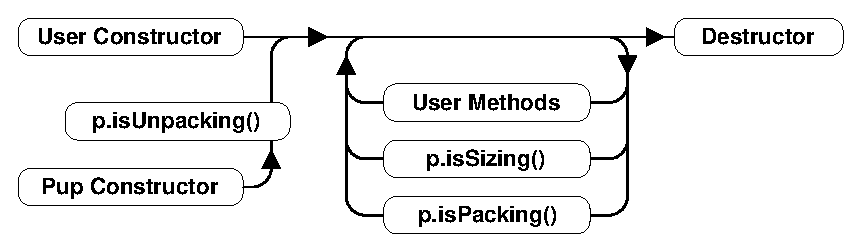
\includegraphics[width=6.0in]{fig/pup}
\end{center}
\caption{Method sequence of an object with a pup method.}
\label{fig:pup}
\end{figure}

Typical method invocation sequence of an object with a pup method is shown in 
Figure~\ref{fig:pup}.  As usual in \CC{}, objects are 
constructed, do some processing, and are then destroyed.

Objects can be created in one of two ways: they can
be created using a normal constructor as usual; or they
can be created using their pup constructor.  The pup constructor
for \charmpp{} array elements and \kw{PUP::able} objects
is a ``migration constructor'' that takes a single ``CkMigrateMessage *";
for other objects, such as parameter marshalled objects,
the pup constructor has no parameters.  The pup constructor
is always followed by a call to the object's pup method in
\verb.isUnpacking. mode.

Once objects are created, they respond to regular user methods
and remote entry methods as usual.  At any time, the object 
pup method can be called in \verb.isSizing. or \verb.isPacking.
mode.  User methods and sizing or packing pup methods can be called
repeatedly over the object lifetime.

Finally, objects are destroyed by calling their destructor
as usual.


\section{Migratable Array Elements using PUP}

\label{arraymigratable}
Array objects can \index{migrate}migrate from one PE to another.  For
example, the load balancer (see section~\ref{lbFramework}) might
migrate array elements to better balance the load between processors.
% The following are no longer strictly true - an unimplemented PUP is
% a no-op, and chare PUPs no longer need to call their base class's
% PUP
For an array element to be migratable, it must implement a \uw{pup}
method.  The standard PUP contract (see section \ref{sec:pupcontract})
and constraints wrt to serializing data apply. The one exception for chare
, group and node group types is that since the runtime system will be the
one to invoke their PUP routines, the runtime will automatically call PUP
on the generated CBase\_ superclasses so users do not need to call PUP on
generated superclasses.

A simple example for an array follows:

\begin{alltt}
//In the .h file:
class A2 : public CBase\_A2 \{
private: //My data members:
    int nt;
    unsigned char chr;
    float flt[7];
    int numDbl;
    double *dbl;
public:	
    //...other declarations

    virtual void pup(PUP::er \&p);
\};

//In the .C file:
void A2::pup(PUP::er \&p)
\{
    // The runtime will automatically call CBase\_A2::pup()
    p|nt;
    p|chr;
    p(flt,7);
    p|numDbl;
    if (p.isUnpacking()) dbl=new double[numDbl];
    p(dbl,numDbl);
\}
\end{alltt}

The default assumption, as used in the example above, for the object
state at PUP time is that a chare, and its member objects, could be
migrated at any time while it is inactive, i.e. not executing an entry
method.  Actual migration time can be controlled (see
section~\ref{lbFramework}) to be less frequent.  If migration timing
is fully user controlled, e.g., at the end of a synchronized load
balancing step, then PUP implementation can be simplified to only
transport ``live'' ephemeral data matching the object state which
coincides with migration.  More intricate state based PUPing, for
objects whose memory footprint varies substantially with computation
phase, can be handled by explicitly maintaining the object's phase in
a member variable and implementing phase conditional logic in the PUP
method (see section~\ref{sec:pupdynalloc}).

\section{Marshalling User Defined Data Types via PUP}

Parameter marshalling requires serialization and is therefore
implemented using the PUP framework.  User defined data types passed
as parameters must abide by the standard PUP contract (see section
\ref{sec:pupcontract}).

A simple example of using PUP to marshall user defined data types follows:

\begin{alltt}
class Buffer \{
public:
//...other declarations
  void pup(PUP::er &p) \{
    // remember to pup your superclass if there is one
    p|size;
    if (p.isUnpacking())
      data = new int[size];
    PUParray(p, data, size);
  \}

private:
  int size;
  int *data;
\};


// In some .ci file
entry void process(Buffer &buf);
\end{alltt}

For efficiency, arrays are always copied as blocks of bytes and passed
via pointers.  This means classes that need their pup routines to be
called, such as those with dynamically allocated data or virtual
methods cannot be passed as arrays--use STL vectors to pass
lists of complicated user-defined classes.  For historical reasons,
pointer-accessible structures cannot appear alone in the parameter
list (because they are confused with messages).

The order of marshalling operations on the send side is:
\begin{itemize}
\item Call ``p\verb.|.a'' on each marshalled parameter with a sizing PUP::er.
\item Compute the lengths of each array.
\item Call ``p\verb.|.a'' on each marshalled parameter with a packing PUP::er.
\item \kw{memcpy} each arrays' data.
\end{itemize}

The order of marshalling operations on the receive side is:
\begin{itemize}
\item Create an instance of each marshalled parameter using its default constructor.
\item Call ``p\verb.|.a'' on each marshalled parameter using an unpacking PUP::er.
\item Compute pointers into the message for each array.
\end{itemize}

Finally, very large structures are most efficiently passed via messages,
because messages are an efficient, low-level construct that minimizes copying
and overhead; but very complicated structures are often most easily passed via 
marshalling, because marshalling uses the high-level pup framework.

See \examplerefdir{PUP/HeapPUP}


  \subsection{Terminal I/O}

\index{input/output}
\charmpp\ provides both C and \CC\ style methods of doing terminal I/O.  

In place of C-style printf and scanf, \charmpp\ provides
\kw{CkPrintf} and \kw{CkScanf}.  These functions have
interfaces that are identical to their C counterparts, but there are some
differences in their behavior that should be mentioned.

\function{int CkPrintf(format [, arg]*)} \index{CkPrintf} \index{input/output}
\desc{This call is used for atomic terminal output. Its usage is similar to
\texttt{printf} in C.  However, \kw{CkPrintf} has some special properties
that make it more suited for parallel programming on networks of
workstations.  \kw{CkPrintf} routes all terminal output to the \kw{charmrun},
which is running on the host computer.  So, if a
\index{chare}chare on processor 3 makes a call to \kw{CkPrintf}, that call
puts the output in a TCP message and sends it to host
computer where it will be displayed.  This message passing is an asynchronous
send, meaning that the call to \kw{CkPrintf} returns immediately after the
message has been sent, and most likely before the message has actually
been received, processed, and displayed. \footnote{Because of
communication latencies, the following scenario is actually possible:
Chare 1 does a \kw{Ckprintf} from processor 1, then creates chare 2 on
processor 2.  After chare 2's creation, it calls \kw{CkPrintf}, and the
message from chare 2 is displayed before the one from chare 1.}
}

\function{void CkError(format [, arg]*))} \index{CkError} \index{input/output} 
\desc{Like \kw{CkPrintf}, but used to print error messages on \texttt{stderr}.}

\function{int CkScanf(format [, arg]*)} \index{CkScanf} \index{input/output}
\desc{This call is used for atomic terminal input. Its usage is similar to
{\tt scanf} in C.  A call to \kw{CkScanf}, unlike \kw{CkPrintf},
blocks all execution on the processor it is called from, and returns
only after all input has been retrieved.
}

For \CC\ style stream-based I/O, \charmpp\ offers \kw{ckin},
\kw{ckout}, and \kw{ckerr} in the place of cin, cout, and cerr.  The
\CC streams and their \charmpp\ equivalents are related in the same
manner as printf and scanf are to \kw{CkPrintf} and \kw{CkScanf}.  The
\charmpp\ streams are all used through the same interface as the \CC\ 
streams, and all behave in a slightly different way, just like C-style
I/O. \kw{ckout} and \kw{ckerr} both have the same idiosyncratic
behavior as \kw{CkPrintf}, and \kw{ckin} behaves in the same way as
\kw{CkScanf}.

  \subsection{Other Calls}

\label{other Charm++ calls}

The following calls provide information about the machines upon which the
parallel program is executing.  Processing Element refers to a single CPU.
Node refers to a single machine-- a set of processing elements which share
memory (i.e. an address space).  Processing Elements and Nodes are numbered,
starting from zero.

Thus if a parallel program is executing on one 4-processor workstation and one
2-processor workstation, there would be 6 processing elements (0, 1 ,2, 3, 4,
and 5) but only 2 nodes (0 and 1).  A given node's processing elements are
numbered sequentially.

{\bf int CkNumPes()} \index{CkNumPes} \\
returns the total number of processors, across all nodes.

{\bf int CkMyPe()} \index{CkMyPe} \\
returns the processor number on which the call was made.

{\bf int CkMyRank()} \index{CkMyRank} \\
returns the rank number of the processor on which the call was made.
Processing elements within a node are ranked starting from zero.

{\bf int CkMyNode()} \index{CkMyNode} \\
returns the address space number (node number) on which the call was made.

{\bf int CkNumNodes()} \index{CkMyNodes} \\
returns the total number of address spaces.

{\bf int CkNodeFirst(int node)} \index{CkNodeFirst} \\
returns the processor number of the first processor in this address space.

{\bf int CkNodeSize(int node)} \index{CkNodeSize} \\
returns the number of processors in the address space on which the call was made.

{\bf int CkNodeOf(int pe)} \index{CkNodeOf} \\
returns the node number on which the call was made.

{\bf int CkRankOf(int pe)} \index{CkRankOf} \\
returns the rank of the given processor within its node.

The following calls provide commonly needed functions.

{\bf void CkAbort(const char *message)} \index{CkAbort} \\
Cause the program to abort, printing the given error message.

{\bf void CkExit()} \index{CkExit} \\
This call informs the Charm kernel that computation on all processors should 
terminate.  After the currently executing entry method completes, no more 
messages or entry methods will be called.  \keyword{CkExit()} should be the 
last statement of the entry method from which it was called. 

{\bf int CkTimer()} \index{CkTimer} \index{timers} \\
returns the current value of the system timer in milliseconds. The system
timer is started when \\
the program begins execution. This timer measures
process time (user and system).

{\bf double CkWallTimer()} \index{CkWallTimer} \index{timers} \\
returns the elapsed time since the program has started from the wall clock 
timer.

    
  \subsection{Delegation}

\index{Delegation}
\label{delegation}

{\em Delegation} is a means by which a library writer can 
intercept messages sent via a proxy.  This is typically
used to construct communication libraries.
A library creates a special kind of Group called a 
\kw{DelegationManager}, which receives the messages
sent via a delegated proxy.

There are two parts to the delegation interface-- a
very small client-side interface to enable delegation,
and a more complex manager-side interface to handle
the resulting redirected messages.

\subsubsection{Client Interface}

All proxies (Chare, Group, Array, ...) in \charmpp\ 
support the following delegation routines.

\function{void CProxy::ckDelegate(CkGroupID delMgr);}
Begin delegating messages sent via this proxy to the
given delegation manager. This only affects
the proxy it is called on-- other proxies for the
same object are {\em not} changed. If the proxy is 
already delegated, this call changes the delegation manager.

\function{CkGroupID CProxy::ckDelegatedIdx(void) const;}
Get this proxy's current delegation manager.

\function{void CProxy::ckUndelegate(void);}
Stop delegating messages sent via this proxy.  
This restores the proxy to normal operation.

One use of these routines might be:

\begin{alltt}
  CkGroupID mgr=somebodyElsesCommLib(...);
  CProxy_foo p=...;
  p.someEntry1(...); //Sent to foo normally
  p.ckDelegate(mgr);
  p.someEntry2(...); //Handled by mgr, not foo!
  p.someEntry3(...); //Handled by mgr again
  p.ckUndelegate();
  p.someEntry4(...); //Back to foo
\end{alltt}

The client interface is very simple; but it is often
not called by users directly.  Often the delegate 
manager library needs some other initialization,
so a more typical use would be:

\begin{alltt}
  CProxy_foo p=...;
  p.someEntry1(...); //Sent to foo normally
  startCommLib(p,...); // Calls ckDelegate on proxy
  p.someEntry2(...); //Handled by library, not foo!
  p.someEntry3(...); //Handled by library again
  finishCommLib(p,...); // Calls ckUndelegate on proxy
  p.someEntry4(...); //Back to foo
\end{alltt}

Sync entry methods, group and nodegroup multicast messages,
and messages for virtual chares that have not yet been created
are never delegated.  Instead, these kinds of entry methods
execute as usual, even if the proxy is delegated.

\subsubsection{Manager Interface}

A delegation manager is a group which inherits from
\kw{CkDelegateMgr} and overrides certain virtual methods. 
Since \kw{CkDelegateMgr} does not do any communication itself, 
it need not be mentioned in the
.ci file; you can simply declare a group as usual and
inherit the C++ implementation from \kw{CkDelegateMgr}.

Your delegation manager will be called by \charmpp{}
any time a proxy delegated to it is used.  Since
any kind of proxy can be delegated, there are separate
virtual methods for delegated Chares, Groups, NodeGroups,
and Arrays.

\begin{alltt}
class CkDelegateMgr : public Group {
public:
  virtual void ChareSend(int ep,void *m,const CkChareID *c,int onPE);

  virtual void GroupSend(int ep,void *m,int onPE,CkGroupID g);
  virtual void GroupBroadcast(int ep,void *m,CkGroupID g);

  virtual void NodeGroupSend(int ep,void *m,int onNode,CkNodeGroupID g);
  virtual void NodeGroupBroadcast(int ep,void *m,CkNodeGroupID g);

  virtual void ArrayCreate(int ep,void *m,const CkArrayIndex &idx,int onPE,CkArrayID a);
  virtual void ArraySend(int ep,void *m,const CkArrayIndex &idx,CkArrayID a);
  virtual void ArrayBroadcast(int ep,void *m,CkArrayID a);
  virtual void ArraySectionSend(int ep,void *m,CkArrayID a,CkSectionID &s);
};
\end{alltt}

These routines are called on the send side only.  They are called after 
parameter marshalling; but before the messages are packed.
The parameters passed in have the following descriptions.

\begin{enumerate}
\item{{\bf ep} The entry point begin called, passed as an index into the
\charmpp{} entry table.  This information is also stored in the message's
header; it is duplicated here for convenience.}
\item{{\bf m} The \charmpp{} message.  This is a pointer to the start of the
user data; use the system routine \kw{UsrToEnv} to get the corresponding envelope.
The messages are not necessarily packed; be sure to use \kw{CkPackMessage}.}
\item{{\bf c} The destination \kw{CkChareID}.  This information is already
stored in the message header.}
\item{{\bf onPE} The destination processor number. For chare messages, this
indicates the processor the chare lives on.  For group messages, this indicates
the destination processor.  For array create messages, this indicates the 
desired processor.}
\item{{\bf g} The destination \kw{CkGroupID}.  This is also stored in the 
message header.}
\item{{\bf onNode} The destination node.}
\item{{\bf idx} The destination array index.  This may be looked up using
the lastKnown method of the array manager, e.g., using:
  \begin{alltt}
  int lastPE=CProxy_CkArray(a).ckLocalBranch()->lastKnown(idx);
  \end{alltt} }
\item{{\bf s} The destination array section.}
\end{enumerate}


The \kw{CkDelegateMgr} superclass implements all these methods; so
you only need to implement those you wish to optimize.  You can
also call the superclass to do the final delivery after you've
sent your messages.



    
  \subsection{Communication Optimizations Framework}

The communications framework in Charm++/Converse is aimed at optimizing certain
communication patterns. Currently the programmer has to specify the
communication pattern it intends to optimize, together with the strategy to be
used. The communications library uses the delegation framework in order too
enable easy and transparent access to the framework by the programmer.

For \ampi{} programs, the communication optimization is done by the \ampi{}
layer, so that the user does not need to worry about that. In Charm++, however,
the user must create the strategies in the program explicitly. Charm++ programs
are normally based on communicating arrays of chares, that compute and then
invoke entry methods on local or remote chares by sending them messages. These
array elements send messages to each other through proxies. The messages are
passed to the Charm++ runtime which calls lower level network APIs to
communicate. To optimize communication in Charm++, the user can redirect a
communication {\em call} to go through an instance of a strategy.

To access the communication framework, the user first creates and initializes a
communication library strategy. He then needs to make a copy of the array proxy
and associate it with that strategy. The user can create several instances of
the same strategy, to optimize different communication calls in his application.
Each communication operation is now associated with a proxy. There exist two
interfaces, which need to keep different information in every chare. The first
one is suggested to be used, as it is newer and simpler. The second one is
mainly for reference on older codes.

The information to be kept can be either stored as a readonly variable, or
internally as a private variable of each chare using it.

\subsubsection{Proxy interface}

A proxy containing the delegation should be kept, and reused every time the
associated stragety wants to be used.

\begin{enumerate}
\item main.C global
\begin{verbatim}
// Include the appropriate header file
#include <EachToManyMulticastStrategy.h>
#include <StreamingStrategy.h>

// Declare the global variable
CProxy_MyArray aproxy;
CProxy_MyArray dproxy;
\end{verbatim}

\item main.C:main()
\begin{verbatim}
// Create the array
aproxy = CProxy_Hello::ckNew();

// Create the strategy
Strategy *strategy = new EachToManyStrategy(USE_MESH, srcarray, destarray);
//or
Strategy *strategy = new StreamingStrategy(10,10);

// Register the strategy to a new proxy, so that aproxy is without commlib,
// while dproxy uses it
dproxy = aproxy;
ComlibAssociateProxy(dproxy, strategy);
\end{verbatim}

\item In the array element
\begin{verbatim}
// First proxy should be delegated
ComlibBeginIteration(aproxy);   // Only for bracketed strategies
dproxy[index].entry(message);   // Sending a message
.....     //sending more messages
.....
aproxy[index].entry2{message2); // Send a message without commlib
ComlibEndIteration(aproxy);     // Only for bracketed strategies
\end{verbatim}
\end{enumerate}

The above example shows the usage of EachToManyStrategy. Notice the
ComlibBeginIteration and ComlibEndIteration calls, needed for bracketed
strategies. The construction of the strategies has been done in tha main::main,
from where they are broadcasted and initialized in every processor before being
used.

\subsubsection{Instance interface}

In this interface, the chares need to keep information about the commlib instance.

\begin{enumerate}
\item main.C global
\begin{verbatim}
// Include the appropriate header file
#include <EachToManyMulticastStrategy.h>
#include <StreamingStrategy.h>

// Declare the global variable
CProxy_MyArray aproxy;
ComlibInstanceHandle cinst;
\end{verbatim}

\item main.C:main()
\begin{verbatim}
// Create the array
aproxy = CProxy_Hello::ckNew();

// Create your strategy
Strategy *strategy = new EachToManyStrategy(USE_MESH, srcarray, destarray);
//or
Strategy *strategy = new StreamingStrategy(10,10);

// Create a Communication Library Instance
cinst = CkGetComlibInstance();

// Register the strategy
cinst.setStrategy(strategy);
\end{verbatim}

\item In the array element 
\begin{verbatim}
// Before calling an entry method whose message should go thorough the
// library the proxy has to be delegated. Create a new copy of the
// proxy and delegate it before using it.
CProxy_Hello dproxy = aproxy;
ComlibDelegateProxy(&dproxy); //Now all calls to dproxy will go through the library.

cinst.beginIteration();       // Only for bracketed strategies
dproxy[index].entry();        // Send a message
.....
.....
aproxy[index].entry2();       // Send a message without commlib
cinst.endIteration();         // Only for bracketed strategies
\end{verbatim}
\end{enumerate}

\subsubsection{Sections}

In order to multicast only to a part of the array instead of the entire array,
it is necessary to create a {\textrm{CProxySection\_class}} of the desired
portion of the destination array, delegate it with either
{\textrm{ComlibAssociateProxy()}} or {\textrm{ComlibDelegateProxy}}, and send a
broadcast to it. This broadcast on the section will result in the desired
multicast on the global array.

\subsubsection{Loadbalancing and Migration support}

The Communication optimization framework supports both loadbalancing and array
migration. It enables migration through message forwarding. Messages sent by a
migrated array are forwarded to the processor where it is mapped to, and from
here they get accounted. Messages sent to migrated arrays are forwarded from the
processor where they are mapped to their current destination.

This mapping of array elements to processors can be updated by the user by
calling {\textrm{ComlibResetProxy}} for array proxies, and
{\textrm{ComlibResetSectionProxy}} for section proxies. This should be done
especially during load-balancing, where most of the migrations happen. As shown
in the following example, these calls should be made inside the
{\textrm{resumeFromSync}} method.

At {\em load-balancing} time the user should make comlib remap the array
element. This can be done by calling ComlibResetProxy for array proxies and
ComlibResetSectionProxy for section proxies. This calls need to be made in
resumeFromSync.

\begin{verbatim}
  void arrayelement::resumeFromSync() {
      .......
      .......
      ComlibResetProxy(aproxy);  // Proxy interface
      cinst.setSourcePe();       // Instance interface

      ComlibResetSectionProxy(sproxy);  // Both interfaces
  }
\end{verbatim}

A migrating array element containing {\em associated proxies} or {\em
instances} should pup them all at the source and destination.

\begin{verbatim}
  void arrayelement::pup(PUP::er &p){
      ..........
      ..........
      p | aproxy;
      p | cinst;
  }
\end{verbatim}

\subsubsection{Compiling User Code}

All user programs that use the communcation library should use the
linker option {\textrm{-module comlib}. For example,
\begin{verbatim}
charmc -o pgm pgm.o -module comlib
\end{verbatim}

\subsubsection{Supported Operations and Strategies}

The communication framework now supports four different communication
operations:
\begin{enumerate}
\item many-to-many communication,
\item array and group broadcast,
\item section multicast,
\item streaming.
\end{enumerate}
Table~\ref{tbl:com_operation} shows the different strategies that optimize these
communication operations. Some of these are converse strategies while others are
charm strategies. In the following paragraphs, we present in detail the
strategies optimizing the above mentioned operations.


\begin{table}[h]
\begin{center}
\begin{small}
\begin{tabular}{|c|c|c|}
\hline
{\bf Operation} & {\bf Object Strategy} & {\bf Processor Strategy} \\
\hline
\begin{tabular}{c}
All-to-All/Many-to-many \\
personalized and multicast
\end{tabular}
 & EachToManyMulticastStrategy & Mesh, Grid, Hypercube, Direct \\
%Many-to-many  multicast    & EachToManyMulticastStrategy & Mesh, Grid, Hypercube, Direct \\
Broadcast  & BroadcastStrategy, PipeBroadcastStrategy & Binomial tree, Binary tree\\
Section Multicast & DirectSection, RingSection, TreeSection & \\
Streaming  & Streaming, MeshStreaming, PrioStreaming & \\
\hline
\end{tabular}
\end{small}
\end{center}
\caption{Communication Operations supported in the Framework}
\label{tbl:com_operation}
\end{table}

There are two types of strategies in the communication framework:

\begin{itemize}

\item Bracketed Strategies. In bracketed strategies each source Chare
(which could be an array element or a group) deposits its entries and then the
strategy performs the communication optimization. For example the
EachToManyMulticastStrategy is a bracketed strategy. For bracketed strategies a
beginIteration and an endIteration must be called before and after making the
deposits respectively.

\item Non-Bracketed Strategies. Non-bracketed strategies perform communication
optimizations without needing calls to beginIteration and endIteration to start
processing. Non-bracketed strategies either immediately process messages or
after a timeout, and, in both cases, it's not triggered from the application.

\end{itemize}

\subsubsection{Many-to-many Strategies}

The class {\em EachToManyMulticastStrategy} optimizes both all-to-all
personalized and all-to-all multicast communication using several virtual
topologies like 2-D Mesh, 3-D Mesh and Hypercube. Personalized communication
happens when a chare sends different messages to the other chares, multicast
communication happens when a chare sends the same message to all other chares.
EachToManyMulticastStrategy also optimized the special cases many-to-many where
not all the chares in an array are involved in the collective operation.

The charm level strategy collects all the messages from the chares and delivers
them tos the destination, while the low level (processor-to-processor) communication
is performed through converse level {\em routers}, which implements the various
virtual topologies.

%For example, with the mesh router, the strategy on each processor
%first sends messages to its row neighbors. After having received its row
%messages each processor sends the column messages. After having received the
%column messages an iteration of the strategy finishes. All local messages are
%delivered as soon they are received.

%{\em EachToManyMulticastStrategy} is also used to optimize all-to-all multicast
%communication, where a processor sends the same message to all others, using the
%same virtual topologies at the lower level.

EachToManyMulticastStrategy requires that all local messages be deposited
before they can be packed into single messages. Hence, it needs to be a {\em
bracketed} strategy.

This strategy can also be used to optimize all-to-all collectives between charm
groups.

%Bracketed strategies require each of the participating objects to deposit their
%intended messages within brackets. Calls to {\em ComlibBeginIteration} and {\em
%ComlibEndIteration} create a bracket. The call ComlibBeginIteration sets up the
%delegation framework to forward user messages to the correct strategy instance.
%User messages then get passed to the insertMessage entry function of the
%strategy. When all local objects have called ComlibEndIteration, doneInserting
%is invoked on the strategy.

%Bracketed strategies are typically needed when the communication
%optimization requires local source objects to reach a barrier. At this
%local barrier the communication framework invokes doneInserting on
%that strategy, which the calls the converse level strategy.

%Non-bracketed strategies have no such restriction. They process
%messages as soon as they arrive. so, non-bracketed strategies should
%not expect a doneInserting to be invoked on them. They must all
%process messages in the insertMessage call itself.

As for the constructors to be used in the main chare, the two prototypes follow.
The first one is for groups, the second for arrays. The optional parameters
allow to specify the many-to-many behaviour, passing the lists of source and
destination elements participating in the operation. If they are left to the
default value, the collective is an all-to-all.

\begin{verbatim}
EachToManyMulticastStrategy(int substrategy, int nsrcpes=0, int *srcpelist=0,
                            int ndestpes=0, int *destpelist=0);

EachToManyMulticastStrategy(int substrategy, CkArrayID src, CkArrayID dest,
                            int nsrc=0, CkArrayIndexMax *srcelements=0,
                            int ndest=0, CkArrayIndexMax *destelements=0);
\end{verbatim}

Both have as first parameter the virtual topology that the strategy will use for
the low level optimization. The possible values are:

\begin{description}
\item[USE\_DIRECT] to send messages directly;
\item[USE\_MESH] to send messages across a 2D Mesh;
\item[USE\_GRID] to send messages across a 3D Grid;
\item[USE\_HYPERCUBE] to send messages across a Hypercube.
\end{description}

USE\_HYPERCUBE will do best for very small messages and small number of
processors, 3d has better performance for slightly higher message sizes and then
Mesh starts performing best. The programmer is encouraged to try out all the
topologies.

The header file to include is {\textrm{EachToManyMulticastStrategy.h}}.

\subsubsection{Broadcast Strategies}

There are two strategies of this type: {\em BroadcastStrategy} and {\em
PipeBroadcastStrategy}. The first works only for group broadcast, while the
second works for both groups and arrays.

BroadcastStrategy performs a broadcast through a hypercube (default) or a tree,
and the constructor is:

\begin{verbatim}
BroadcastStrategy(int topology=USE_HYPERCUBE);
\end{verbatim}

PipeBroadcastStrategy performs a broadcast through a ring or a hypercube
(default). The characteristic of this strategy is that it fragments the message
into small chunks that fit a predetermined size (passed as argument to the
constructor), and it reassembles it before delivery. The constructor prototypes
for groups and arrays respectively are:

\begin{verbatim}
  PipeBroadcastStrategy(int topology, CkArrayID aid, int pipeSize=DEFAULT_PIPE);

  PipeBroadcastStrategy(CkGroupID gid, int topology=USE_HYPERCUBE, int pipeSize=DEFAULT_PIPE);
\end{verbatim}

The header file to include is {\textrm{BroadcastStrategy.h}} or
{\textrm{PipeBroadcastStrategy.h}}, depending on which strategy is used.

\subsubsection{Section Multicast Strategies}

The DirectMulticastStrategy and its subclasses can multicast a message to the entire
array or a section of array elements. The direct multicast strategies
are non-bracketed, and the message is processed when the application
deposits is. These strategies do not combine messages, but they may
sequence the destinations of the multicast to minimize contention on a
network.

These are the subclass strategies that are available:

\begin{description}
\item[KDirectMulticastStrategy] sends the messages along a spanning tree of factor {\em k};
\item[RingMulticastStrategy] sends the messages along ring resulting in good throughput as the ring permutation is contention free on many communication topologies;
\item[MultiRingMulticast] sends the messages along a ring with multiple start points on the ring.
\end{description}

For these, the constructors are of the form:

\begin{verbatim}
KDirectMulticastStrategy(int kfactor, CkArrayID aid);

RingMulticastStrategy(CkArrayID dest_id, int flag=0);

MultiRingMulticast(CkArrayID dest_id, int flag=0);
\end{verbatim}

For section multicast, the user must create a section proxy and delegate it to
the communication library. Invocations on section proxies are passed on to the
section multicast strategy.

The header file to include is respective to the strategy name.

\subsubsection{Streaming Strategies}

This strategy optimizes the scenario where chares send several small messages to
other chares. The StreamingStrategy collects messages destined to the same
processor and, after a timeout or when a certain number of messages have been
collected, it sends them as a single message. This results in sending fewer
messages of larger size. The timeout is a floating-point parameter to the
StreamingStrategy. It needs to be specified in milliseconds, with a default
value of 1ms. Micro-second timeouts can also be specified by passing values less
than 1. For example, $0.1$ represents $100\mu s$.

The Streaming Strategy is a non-bracketed strategy, so there is no need to call
{\textrm{beginIteration}} and {\textrm{endIteration}}. Since messages can be
delayed due to the timeout present, it is possible to call
{\textrm{endIteration}} to flush all the messages to be sent immediately.

The prototype of the constructor is:

\begin{verbatim}
Strategy * strategy = new StreamingStrategy(float period\_in\_ms, int nmsgs);
\end{verbatim}

There are two variants of this strategy:

\begin{description}
\item[MeshStreamingStrategy] which sends the messages along a mesh instead of a linear array as the basic one;
\item[PrioStreaming] which looks at the priority of the messages, and sends those with a priority above a certain threshold directly, without delay. This strategy accepts a third parameter in the constructor for the threshold priority.
\end{description}

The header file to include is respective to the strategy name.

\subsubsection{Communication Optimization Development}

Optimization algorithms are implemented as Strategies in the communication
library. Strategies can be implemented at the Object (\charmpp) level or the
processor (\converse) level. Code reuse is possible by having a few object
managers perform object level optimizations and then call several other
processor level optimization schemes. For example, to optimize all-to-all
communication the processor level strategies could use the different virtual
topologies.

All processor (\converse) level strategies inherit from the {\em class~Strategy}
defined below and override its virtual methods.

\begin{verbatim}
// Converse or Processor level strategy
class Strategy : public PUP::able{
public:
    // Called for each message
    virtual void insertMessage(MessageHolder *msg);
    // Called after all chares and groups have finished depositing their
    // messages on that processor.

    virtual void doneInserting();
    virtual void beginProcessing(int nelements);
};
\end{verbatim}

The class method {\em insertMessage} is called to deposit messages with the
strategy. MessageHolder is a wrapper for converse messages. When a processor has
sent all its messages {\em doneInserting} is invoked on the strategy.

At the \charmpp{} level, all strategies inherit from the {\em
class~CharmStrategy} reported here.

\begin{verbatim}
// Charm++ or Object level strategy
class CharmStrategy : public Strategy{
 protected:
    int isArray;
    int isGroup;
    int isStrategyBracketed;
    ............   
    ............   
public:
    // Called for each message
    virtual void insertMessage(CharmMessageHolder *msg);
    // Called after all chares and groups have finished depositing their
    // messages on that processor.
    virtual void doneInserting();
    virtual void beginProcessing(int nelements);
};
\end{verbatim}

\charmpp{} level strategies also have to implement the insertMessage and
doneInserting methods. Here insertMessage takes a CharmMessageHolder which is a
\charmpp{} message wrapper. The call to beginProcessing initializes the strategies
on each processor. This additional call is needed because the constructor of the
strategy is called by user code in main::main on processor 0, while the strategy
needs to be constructed everywhere. Along with initializing its data,
beginProcessing can also register message handlers, as the communication library
strategies use Converse handlers to communicate between processors. The flags
{\em isArray} and {\em isGroup} store the type of objects that call the strategy
and the flag {\em isStrategyBracketed} specifies if the CharmStrategy is
bracketed or not. Bracketed strategies require that the application deposits
messages in brackets demarcated by the calls ComlibBeginIteration and
ComlibEndIteration.

  The Python scripting language in \charmpp{} allows the user to dynamically
execute pieces of code inside a running application, without the need to
recompile. This is performed through the CCS (Converse Client Server) framework
(see ``Converse Manual'' for more information about this). The user specifies
which elements of the system will be accessible through the interface, as we
will see later, and then run a client which connects to the server.

In order to exploit this functionality, Python interpreter needs to be installed
into the system, and \charmpp{} LIBS need to be built with:\\
\texttt{./build LIBS $<$arch$>$ $<$options$>$}

The interface provides three different types of requests:

\begin{description}
\item[Execute] requests to execute a code, it will contain the code to be executed on the server, together with the instructions on how to handle the environment;
\item[Print] asks the server to send back all the strings which have been printed by the script until now;
\item[Finished] asks the server if the current script has finished or it is still running.
\end{description}

There are three modes to run code on the server, ordered here by increase of
functionality, and decrease of dynamic flexibility:
\begin{itemize}
\item \textbf{simple read/write} By implementing the \kw{read} and \kw{write} methods
of the object exposed to python, in this way single variables may be exposed,
and the code will have the possibility to modify them individually as desired.
(see section~\ref{pythonServerRW})
\item \textbf{iteration} By implementing the iterator functions in the server (see
\ref{pythonServerIterator}), the user can upload the code of a Python function
and a user-defined iterator structure, and the system will apply the specified
function to all the objects reflected by the iterator structure.
\item \textbf{high level} By implementing \kw{python} entry methods, the Python code uploaded can access them and activate complex, parallel operations that will be performed by the \charmpp{} application. (see section~\ref{pythonHighLevel})
\end{itemize}

This documentation will describe the client API first, and then the server API. 


\section{Client API}

\label{pythonClient}

In order to facilitate the interface between the client and the server, some
classes are available to the user to include into the client. Currently \CC{} and
java interfaces are provided.

\CC{} programs need to include \texttt{PythonCCS-client.h} into their
code. This file is among the \charmpp{} include files. For java, the package
\texttt{charm.ccs} needs to be imported. This is located under the java
directory on the \charmpp{} distribution, and it provides both the Python and
CCS interface classes.

There are three main classes provided: \texttt{PythonExecute},
\texttt{PythonPrint}, and \texttt{PythonFinished} which are used for the three
different types of request.

All of them have two common methods to enable communication across different platforms:

\begin{description}

\item[int size();]
Returns the size of the class, as number of bytes that will be
transmitted through the network (this includes the code and other dynamic
variables in the case of \texttt{PythonExecute}).

\item[char *pack();]
Returns a new memory location containing the data to be sent to the server, this
is the data which has to be passed to the \texttt{CcsSendRequest} function. The
original class will be unmodified and can be reused in subsequent calls.

\end{description}

A typical invocation to send a request from the client to the server has the
following format:

\begin{alltt}
CcsSendRequest (&server, "pyCode", 0, request.size(), request.pack());
\end{alltt}

\section{PythonExecute}
\label{pythonExecute}

To execute a Python script on a running server, the client has to create an
instance of \texttt{PythonExecute}, the two constructors have the following
signature (java has a corresponding functionality):

\begin{alltt}
PythonExecute(char *code, bool persistent=false, bool highlevel=false, CmiUInt4 interpreter=0);
PythonExecute(char *code, char *method, PythonIterator *info, bool persistent=false,
              bool highlevel=false, CmiUInt4 interpreter=0);
\end{alltt}

The second one is used for iterative requests (see~\ref{pythonIterator}). The
only required argument is the code, a null terminated string, which will not be
modified by the system. All the other parameters are optional. They refer to the
possible variants for an execution request. In particular, this is a
list of all the options:

\begin{description}

\item[iterative]
If the request is a single code (false) or if it represents a function over
which to iterate (true) (see~\ref{pythonIterator} for more details).

\item[persistent]
It is possible to store information on the server which will be
retained across different client calls (from simple data all the way
up to complete libraries). True means that the information will be
retained on the server, false means that the information will be
deleted when the script terminates. In order to properly release the
memory, when the last call is made (and the data is no longer
required), this flag should be set to false. To reuse persistent data,
the interpreter field of the request should be set to handle returned by a previous persistent call (see later in this subsection).

\item[high level]
In order to have the ability to call high level \charmpp{} functions (available
through the keyword \kw{python}) this flag must be set to true. If it is false,
the entire module ``charm'' will not be present, but the startup of the script
will be faster.

\item[print retain]
When the requested action triggers printed output for the client, this data can be
retrieved with a PythonPrint request. If the output is not desired, this flag
can be set to false, and the output will be discarded. If it is set to true the
output will be buffered pending retrieval by the client. The data will
survive also after the termination of the Python script, and if not retrieved
will bloat memory usage on the server.

\item[busy waiting]
Instead of returning a handle immediately to the client, that can be used to
retrieve prints and check if the script has finished, the server will answer to
the client only when the script has terminated to run (and it will effectively
work as a PythonFinished request).

\end{description}

These flags can be set and checked with the following routines (CmiUInt4 represent a 4
byte unsigned integer):

\begin{alltt}
void setCode(char *set);
void setPersistent(bool set);
void setIterate(bool set);
void setHighLevel(bool set);
void setKeepPrint(bool set);
void setWait(bool set);
void setInterpreter(CmiUInt4 i);

bool isPersistent();
bool isIterate();
bool isHighLevel();
bool isKeepPrint();
bool isWait();
CmiUInt4 getInterpreter();
\end{alltt}

From a PythonExecute request, the server will answer with a 4 byte integer
value, which is a handle for the interpreter that is running. It can be used to
request for prints, check if the script has finished, and for reusing the same
interpreter (if it was persistent).

A value of 0 means that there was an error and the script didn't run. This is
typically due to a request to reuse an existing interpreter which is not
available, either because it was not persistent or because another script is
still running on that interpreter.


\section{Auto-imported modules}
\label{pythonModules}

When a Python script is run inside a \charmpp{} application, two Python modules
are made available by the system. One is \textbf{ck}, the other is
\textbf{charm}. The first one is always present and it represent basic
functions, the second is related to high level scripting and it is present only
when this is enabled (see \ref{pythonExecute} for how to enable it, and
\ref{pythonHighLevel} for a description on how to implement charm functions).

The methods present in the \texttt{ck} module are the following:

\begin{description}

\item[printstr]
It accepts a string as parameter. It will write into the server stdout that string
using the \texttt{CkPrintf} function call.

\item[printclient]
It accepts a string as parameter. It will forward the string back to the client when it
issues a PythonPrint request. It will buffer the strings until requested by PythonPrint if the \texttt{KeepPrint}
option is true, otherwise it will discard them.

\item[mype]
Requires no parameters, and will return an integer representing the
current processor where the code is executing. It is equivalent to the \charmpp{}
function \texttt{CkMyPe()}.

\item[numpes]
Requires no parameters, and will return an integer representing the
total number of processors that the application is using. It is equivalent to
the \charmpp{} function \texttt{CkNumPes()}.

\item[myindex]
Requires no parameters, and will return the index of the current element
inside the array, if the object under which Python is running is an array, or
None if it is running under a Chare, a Group or a Nodegroup. The index will be a
tuple containing as many numbers as the dimension of the array.

\item[read]
It accepts one object parameter, and it will perform a read request to the
\charmpp{} object connected to the Python script, and return an object
containing the data read (see \ref{pythonServerRW} for a description of this
functionality). An example of a call can be:
\function{value = ck.read((number, param, var2, var3))}
where the double parenthesis are needed to create a single tuple object
containing four values passed as a single paramter, instead of four different
parameters.

\item[write]
It accepts two object parameters, and it will perform a write request to the
\charmpp{} object connected to the Python script. For a description of this
method, see \ref{pythonServerRW}. Again, only two objects need to be passed, so
extra parenthesis may be needed to create tuples from individual values.

\end{description}

\section{Iterate mode}
\label{pythonIterator}

Sometimes some operations need to be iterated over all the elements in the
system. This ``iterative'' functionality provides a shortcut for the client user
to do this. As an example, suppose we have a system which contains particles,
with their position, velocity and mass. If we implement \texttt{read} and
\texttt{write} routines which allow us to access single particle attributes, we may
upload a script which doubles the mass of the particles with velocity greater
than 1:

\begin{alltt}
size = ck.read((``numparticles'', 0));
for i in range(0, size):
    vel = ck.read((``velocity'', i));
    mass = ck.read((``mass'', i));
    mass = mass * 2;
    if (vel > 1): ck.write((``mass'', i), mass);
\end{alltt}

Instead of all these read and writes, it will be better to be able to write:

\begin{alltt}
def increase(p):
    if (p.velocity > 1): p.mass = p.mass * 2;
\end{alltt}

This is what the ``iterative'' functionality provides. In order for this to
work, the server has to implement two additional functions
(see~\ref{pythonServerIterator}), and the client has to pass some more
information together with the code. This information is the name of the function
that has to be called (which can be defined in the ``code'' or was previously
uploaded to a persistent interpreter), and a user defined structure which
specifies over what data the function should be invoked. These values can be
specified either while constructing the PythonExecute variable (see the second
constructor in section~\ref{pythonExecute}), or with the following methods:

\begin{alltt}
void setMethodName(char *name);
void setIterator(PythonIterator *iter);
\end{alltt}

The \texttt{PythonIterator} object must be defined by the user, and
the user must insure that the same definition is present inside both the
client and the server. The \charmpp{} system will simply pass this structure as
a void pointer. This structure must inherit from \texttt{PythonIterator}.  In the simple case (highly recommended), wherein no pointers or dynamic allocation are used inside this class,  nothing else needs to be done because it is trivial to serialize such objects.

If instead pointers or dynamic memory allocation are used, the following methods
have to be reimplemented to support correct serialization:

\begin{alltt}
int size();
char * pack();
void unpack();
\end{alltt}

The first returns the size of the class/structure after being packed. The second
returns a pointer to a newly allocated memory containing all the packed data,
the returned memory must be compatible with the class itself, since later on
this same memory a call to unpack will be performed. Finally, the third will do
the work opposite to pack and fix all the pointers. This method will not return
anything and is supposed to fix the pointers ``inline''.

\section{PythonPrint}
\label{pythonPrint}

In order to receive the output printed by the Python script, the client needs to
send a PythonPrint request to the server. The constructor is:

\function{PythonPrint(CmiUInt4 interpreter, bool Wait=true, bool Kill=false);}

The interpreter for which the request is made is mandatory. The other parameters
are optional. The wait parameter represents whether a reply will be sent back
immediately to the client even if there is no output (false), or if the answer
will be delayed until there is an output (true). The \kw{kill} option set to
true means that this is not a normal request, but a signal to unblock the latest
print request which was blocking.

The returned data will be a non null-terminated string if some data is present
(or if the request is blocking), or a 4 byte zero data if nothing is present.
This zero reply can happen in different situations:

\begin{itemize}
\item If the request is non blocking and no data is available on the server;
\item If a kill request is sent, the previous blocking request is squashed;
\item If the Python code ends without any output and it is not persistent;
\item If another print request arrives, the previous one is squashed and the second one is kept.
\end{itemize}

As for a print kill request, no data is expected to come back, so it is safe to
call \texttt{CcsNoResponse(server)}.

The two options can also be dynamically set with the following methods:

\begin{alltt}
void setWait(bool set);
bool isWait();

void setKill(bool set);
bool isKill();
\end{alltt}

\section{PythonFinished}
\label{pythonFinished}

In order to know when a Python code has finished executing, especially when
using persistent interpreters, and a serialization of the scripts is needed, a
PythonFinished request is available. The constructor is the following:

\function{PythonFinished(CmiUInt4 interpreter, bool Wait=true);}

The interpreter corresponds to the handle for which the request was sent, while
the wait option refers to a blocking call (true), or immediate return (false).

The wait option can be dynamically modified with the two methods:

\begin{alltt}
void setWait(bool set);
bool isWait();
\end{alltt}

This request will return a 4 byte integer containing the same interpreter value
if the Python script has already finished, or zero if the script is still
running.

\section{Server API}
\label{pythonServer}

In order for a \charmpp{} object (chare, array, node, or nodegroup) to receive
python requests, it is necessary to define it as python-compliant. This is done
through the keyword \kw{python} placed in square brackets before the object name
in the .ci file. Some examples follow:

\begin{alltt}
mainchare [python] main \{\ldots\}
array [1D] [python] myArray \{\ldots\}
group [python] myGroup \{\ldots\}
\end{alltt}

In order to register a newly created object to receive Python scripts, the
method \texttt{registerPython} of the proxy should be called. As an example,
the following code creates a 10 element array myArray, and then registers it to
receive scripts directed to ``pycode''. The argument of \texttt{registerPython}
is the string that CCS will use to address the Python scripting capability of
the object.

\begin{alltt}
Cproxy_myArray localVar = CProxy_myArray::ckNew(10);
localVar.registerPython(``pycode'');
\end{alltt}


\section{Server \kw{read} and \kw{write} functions}
\label{pythonServerRW}

As explained previously in subsection~\ref{pythonModules}, some functions are
automatically made available to the scripting code through the {\em ck} module.
Two of these, \textbf{read} and \textbf{write} are only available if redefined
by the object. The signatures of the two methods to redefine are:

\begin{alltt}
PyObject* read(PyObject* where);
void write(PyObject* where, PyObject* what);
\end{alltt}

The read function receives as a parameter an object specifying from where the data
will be read, and returns an object with the information required. The write
function will receive two parameters: where the data will be written and what
data, and will perform the update. All these \texttt{PyObject}s are generic, and
need to be coherent with the protocol specified by the application. In order to
parse the parameters, and create the value of the read, please refer to the
manual \htmladdnormallink{``Extending and Embedding the Python Interpreter''}{http://docs.python.org/}, and in particular to the functions
\texttt{PyArg\_ParseTuple} and \texttt{Py\_BuildValue}.

\section{Server iterator functions}
\label{pythonServerIterator}

In order to use the iterative mode as explained in
subsection~\ref{pythonIterator}, it is necessary to implement two functions
which will be called by the system. These two functions have the following
signatures:

\begin{alltt}
int buildIterator(PyObject*, void*);
int nextIteratorUpdate(PyObject*, PyObject*, void*);
\end{alltt}

The first one is called once before the first execution of the Python code, and
receives two parameters. The first is a pointer to an empty PyObject to be filled with
the data needed by the Python code. In order to manage this object, some utility
functions are provided. They are explained in subsection~\ref{pythonUtilityFuncs}.

The second is a void pointer containing information of what the iteration should
run over. This parameter may contain any data structure, and an agreement between the
client and the user object is necessary. The system treats it as a void pointer
since it has no information about what user defined data it contains.

The second function (\texttt{nextIteratorUpdate}) has three
parameters. The first parameter contains the object to be filled
(similar to \texttt{buildIterator}), but the second object contains
the PyObject which was provided for the last iteration, potentially
modified by the Python function. Its content can be read with the
provided routines, used to retrieve the next logical element in the
iterator (with which to update the parameter itself), and possibly
update the content of the data inside the \charmpp{} object. The
second parameter is the object returned by the last call to the Python
function, and the third parameter is the same data structure passed
to \texttt{buildIterator}.

Both functions return an integer which will be interpreted by the system as follows:
\begin{description}
\item[1] - a new iterator in the first parameter has been provided, and the Python function should be called with it;
\item[0] - there are no more elements to iterate.
\end{description}

\section{Server utility functions}
\label{pythonUtilityFuncs}

These are inherited when declaring an object as Python-compliant, and therefore
they are available inside the object code. All of them accept a PyObject pointer
where to read/write the data, a string with the name of a field, and one or two
values containing the data to be read/written (note that to read the data from
the PyObject, a pointer needs to be passed). The strings used to identify the
fields will be the same strings that the Python script will use to access the
data inside the object.

The name of the function identifies the type of Python object stored inside the
PyObject container (i.e String, Int, Long, Float, Complex), while the parameter
of the functions identifies the \CC object type.

\begin{alltt}
void pythonSetString(PyObject*, char*, char*);
void pythonSetString(PyObject*, char*, char*, int);
void pythonSetInt(PyObject*, char*, long);
void pythonSetLong(PyObject*, char*, long);
void pythonSetLong(PyObject*, char*, unsigned long);
void pythonSetLong(PyObject*, char*, double);
void pythonSetFloat(PyObject*, char*, double);
void pythonSetComplex(PyObject*, char*, double, double);

void pythonGetString(PyObject*, char*, char**);
void pythonGetInt(PyObject*, char*, long*);
void pythonGetLong(PyObject*, char*, long*);
void pythonGetLong(PyObject*, char*, unsigned long*);
void pythonGetLong(PyObject*, char*, double*);
void pythonGetFloat(PyObject*, char*, double*);
void pythonGetComplex(PyObject*, char*, double*, double*);
\end{alltt}

To handle more complicated structures like Dictionaries, Lists or Tuples, please refer to \htmladdnormallink{``Python/C API Reference Manual''}{http://docs.python.org/}.

\section{High level scripting}
\label{pythonHighLevel}

When in addition to the definition of the \charmpp{} object as \kw{python}, an
entry method is also defined as \kw{python}, this entry method can be accessed
directly by a Python script through the {\em charm} module. For example, the
following definition will be accessible with the python call:
\function{result = charm.highMethod(var1, var2, var3)}
It can accept any number of parameters (even complex like tuples or
dictionaries), and it can return an object as complex as needed.

The method must have the following signature:

\begin{alltt}
entry [python] void highMethod(int handle);
\end{alltt}

The parameter is a handle that is passed by the system, and can be used in
subsequent calls to return values to the Python code. %Thus, if the method
%does not return immediately but it sends out messages to other \charmpp{}
%objects, the handle must be saved somewhere. \textbf{Note:} if another Python
%script is sent to the server, this second one could also call the same function.
%If this is possible, the handle should be saved in a non-scalar variable.

The arguments passed by the Python caller can be retrieved using the function:

\function{PyObject *pythonGetArg(int handle);}

which returns a PyObject. This object is a Tuple containing a vector of all
parameters. It can be parsed using \texttt{PyArg\_ParseTuple} to extract the
single parameters.

When the \charmpp's entry method terminates (by means of \texttt{return} or
termination of the function), control is returned to the waiting Python script.
Since the \kw{python} entry methods execute within an user-level thread, it is
possible to suspend the entry method while some computation is carried on in
\charmpp. To start parallel computation, the entry method can send regular messages,
as every other threaded entry method (see~\ref{libraryInterface} for more
information on how this can be done using CkCallbackResumeThread callbacks). The
only difference with other threaded entry methods is that here the callback
\texttt{CkCallbackPython} must be used instead of CkCallbackResumeThread. The
more specialized CkCallbackPython callback works exactly like the other one,
except that it correctly handles Python internal locks.

At the end of the computation, the following special function will return a value to the Python script:

\function{void pythonReturn(int handle, PyObject* result);}

where the second parameter is the Python object representing the returned value.
The function \texttt{Py\_BuildValue} can be used to create this value. This
function in itself does not terminate the entry method, but only sets the
returning value for Python to read when the entry method terminates.

A characteristic of Python is that in a multithreaded environment (like the one
provided in \charmpp{}), the running thread needs to keep a lock to prevent
other threads to access any variable. When using high level scripting, and the
Python script is suspended for long periods of time while waiting for the
\charmpp{} application to perform the required task, the Python internal locks
are automatically released and re-acquired by the \texttt{CkCallbackPython}
class when it suspends.

\zap{
This can be done using the two functions:

\begin{alltt}
void pythonAwake(int handle);   // to acquire the lock
void pythonSleep(int handle);   // to release the lock
\end{alltt}

Important to remember is that before any Python value is accessed, the Python
interpreter must be awake. This include the functions \texttt{Py\_BuildValue} and
\texttt{PyArg\_ParseTuple}. \textbf{Note:} it is an error to call these functions
more than once before the other one is called.
} % end zap

\section{Inheritance and Templates in Charm++}
\label{inheritance and templates}

\charmpp\ supports inheritance among \charmpp\ objects such as
chares, groups, and messages. This, along with facilities for generic
programming using \CC\ style templates for \charmpp\ objects, is a
major enhancement over the previous versions of \charmpp.

\subsection{Chare Inheritance}
\index{inheritance}

Chare inheritance makes it possible to remotely invoke methods of a base
chare \index{base chare} from a proxy of a derived
chare.\index{derived chare} Suppose a base chare is of type 
\uw{BaseChare}, then the derived chare of type \uw{DerivedChare} needs to be
declared in the \charmpp\ interface file to be explicitly derived from
\uw{BaseChare}. Thus, the constructs in the \texttt{.ci} file should look like:

\begin{alltt}
  chare BaseChare \{
    entry BaseChare(someMessage *);
    entry void baseMethod(void);
    ...
  \}
  chare DerivedChare : BaseChare \{
    entry DerivedChare(otherMessage *);
    entry void derivedMethod(void);
    ...
  \}
\end{alltt}

Note that the access specifier \kw{public} is omitted, because \charmpp\
interface translator only needs to know about the public inheritance,
and thus \kw{public} is implicit. A Chare can inherit privately from other
classes too, but the \charmpp\ interface translator does not need to know
about it, because it generates support classes ({\em proxies}) to remotely
invoke only \kw{public} methods.

The class definitions of both these chares should look like:

\begin{alltt}
  class BaseChare : public Chare \{
    // private or protected data
    public:
      BaseChare(someMessage *);
      void baseMethod(void);
  \};
  class DerivedChare : public BaseChare \{
    // private or protected data
    public:
      DerivedChare(otherMessage *);
      void derivedMethod(void);
  \};
\end{alltt}

Now, it is possible to create a derived chare, and invoke methods of base
chare from it, or to assign a derived chare proxy to a base chare proxy
as shown below:

\begin{alltt}
  ...
  otherMessage *msg = new otherMessage();
  CProxy_DerivedChare *pd = new CProxy_DerivedChare(msg);
  pd->baseMethod();     // OK
  pd->derivedMethod();  // OK
  ...
  Cproxy_BaseChare *pb = pd;
  pb->baseMethod();    // OK
  pb->derivedMethod(); // COMPILE ERROR
\end{alltt}

Note that \CC\ calls the default constructor \index{default constructor} of the
base class from any constructor for the derived class where base class
constructor is not called explicitly. Therefore, one should always provide a
default constructor for the base class, or explicitly call another base
class constructor.

Multiple inheritance \index{multiple inheritance} is also allowed for Chares
and Groups. Often, one should make each of the base classes inherit
``virtually'' from \kw{Chare} or \kw{Group}, so that a single copy of
\kw{Chare} or \kw{Group} exists for each multiply derived class.

Entry methods are inherited in the
same manner as methods of sequential \CC{} objects.  
To make an entry method virtual, just add the keyword \kw{virtual}
to the corresponding chare method-- no change is needed in the interface file.
Pure virtual entry methods also require no special description
in the interface file.


\subsection{Inheritance for Messages}
\index{message inheritance}

Messages cannot inherit from other messages.  A message can, however,
inherit from a regular \CC\ class.  For example:

\begin{alltt}
//In the .ci file:
  message BaseMessage1;
  message BaseMessage2;

//In the .h file:
  class Base \{
    // ...
  \};
  class BaseMessage1 : public Base, public CMessage_BaseMessage1 \{
    // ...
  \};
  class BaseMessage2 : public Base, public CMessage_BaseMessage2 \{
    // ...
  \};
\end{alltt}

Messages cannot contain virtual methods
or virtual base classes unless you use a packed message.
Parameter marshalling has complete support for inheritance, virtual
methods, and virtual base classes via the PUP::able framework.


% ( I think the following is now a lie  OSL 7/5/2001 )  
%Similar to Chares, messages can also be derived from base messages. One needs
%to specify this in the \charmpp\ interface file similar to the Chare
%inheritance specification (that is, without the \kw{public} access specifier.)
%Message inheritance makes it possible to send a message of derived type to the
%method expecting a base class message.


\subsection{Generic Programming Using Templates}
\index{templates}

One can write ``templated'' code for Chares, Groups, Messages and other
\charmpp\  entities using familiar \CC\ template syntax (almost). The \charmpp\
interface translator now recognizes most of the \CC\ templates syntax,
including a variety of formal parameters, default parameters, etc. However, not
all \CC\ compilers currently recognize templates in ANSI drafts, therefore the
code generated by \charmpp\ for templates may not be acceptable to some current
\CC\ compilers\footnote{ Most modern \CC\ compilers belong to one of the two
camps. One that supports Borland style template instantiation, and the other
that supports AT\&T Cfront style template instantiation. In the first, code is
generated for the source file where the instantiation is seen.  GNU \CC\ falls
in this category.  In the second, which template is to be instantiated, and
where the templated code is seen is noted in a separate area (typically a local
directory), and then just before linking all the template instantiations are
generated. Solaris CC 5.0 belongs to this category. For templates to work for
compilers in the first category such as for GNU \CC\ all the templated code
needs to be visible to the compiler at the point of instantiation, that is,
while compiling the source file containing the template instantiation. For a
variety of reasons, \charmpp\ interface translator cannot generate all the
templated code in the declarations file {\tt *.decl.h}, which is included in
the source file where templates are instantiated. Thus, for \charmpp\ generated
templates to work for GNU \CC\ even the definitions file {\tt *.def.h} should
be included in the \CC\ source file. However, this file may contain other
definitions apart from templates that will be duplicated if the same file is
included in more than one source files. To alleviate this problem, we have to
do a little trick. Fortunately, this trick works for compilers supporting both
Borland-style and Cfront-style template instantiation, therefore, code using
this trick will be portable. The trick is to include {\tt *.def.h} with a
preprocessor symbol \kw{CK\_TEMPLATES\_ONLY} defined, whenever templates
defined in an \kw{extern} module are instantiated. If your interface file does
not contain template declarations or definitions, you need not bother about
including {\tt *.def.h} for \kw{extern} modules.  For example, if module {\tt
stlib} contains template definitions, that you may want to instantiate in
another module called {\tt pgm}, then {\tt pgm.C} should include {\tt
stlib.def.h} with \kw{CK\_TEMPLATES\_ONLY} defined. Of course, {\tt
stlib.decl.h} needs to be included at the top of {\tt pgm.C}.  }. 

The \charmpp\ interface file should contain the template
definitions as well as the instantiation. For example, if a message
class \uw{TMessage} is templated with a formal type parameter 
\uw{DType}, then every instantiation of \uw{TMessage} should be specified
in the \charmpp\ interface file. An example will illustrate this better:
\index{template}

\begin{alltt}
  template <class DType=int, int N=3> message TMessage;
  message TMessage<>; // same as TMessage<int,3>
  message TMessage<double>; // same as TMessage<double, 3>
  message TMessage<UserType, 1>;
\end{alltt}

Note the use of default template parameters. It is not necessary for
template definitions and template instantiations to be part of the
same module.  Thus, templates could be defined in one module, and
could be instantiated in another module \index{module}, as long as the
module defining a template is imported into the other module using the
\kw{extern module} construct. Thus it is possible to build a standard
\charmpp\ template library. Here we give a flavor of possibilities:

\begin{alltt}
module SCTL \{
  template <class dtype> message  Singleton;
  template <class dtype> group Reducer \{
    entry Reducer(void);
    entry void submit(Singleton<dtype> *);
  \}
  template <class dtype> chare ReductionClient \{
    entry void recvResult(Singleton<dtype> *);
  \}
\};

module User \{
  extern module SCTL;
  message Singleton<int>;
  group Reducer<int>;
  chare RedcutionClient<int>;
  chare UserClient : ReductionClient<int> \{
    entry UserClient(void);
  \}
\};
\end{alltt}

The \uw{Singleton} message is a template for storing one element of any
\uw{dtype}. The \uw{Reducer} is a group template for a spanning-tree reduction,
which is started by submitting data to the local branch. It also contains a
public method to register the \uw{ReductionClient} (or any of its derived
types), which acts as a callback to receive results of a reduction.


\section{Checkpoint/Restart}

\index{Checkpoint/Restart}
\label{sec:checkpoint}

\charmpp{} offers a range of fault tolerance capabilities through its 
checkpoint/restart mechanism. Usual chare-array-based \charmpp{} applications, 
including AMPI applications, can be checkpointed to disk files and be restarted later from the files.

The basic idea behind this is straightforward: checkpointing an 
application is like migrating its parallel objects from the processors
onto disks, and restarting is the reverse. Thanks to the migration 
utilities like PUP'ing(Section~\ref{sec:pup}), users can decide what 
data to save in checkpoints and how to save them. However, unlike migration (where certain objects do not need a PUP method), checkpoint requires all the objects to implement the PUP method.

Two schemes of fault tolerance protocols are implemented.

\subsection{Disk-based Checkpoint/Restart}

\subsubsection{Checkpointing}

\label{sec:diskcheckpoint}
	The API to checkpoint the application is:

\begin{alltt} 
  void CkStartCheckpoint(char* dirname,const CkCallback& cb);
\end{alltt}

The string {\it dirname} is the destination directory where the checkpoint
files will be stored, and {\it cb} is the callback function which will be
invoked after the checkpoint is done, as well as when the restart is
complete. Here is an example of a typical use:

\begin{alltt} 
  . . .
  CkCallback cb(CkIndex_Hello::SayHi(),helloProxy);
  CkStartCheckpoint("log",cb);
\end{alltt}

A chare array usually has a PUP routine for the sake of migration. 
The PUP routine is also used in the checkpointing and restarting process.
Therefore, it is up to the programmer what to save and restore for
the application. One illustration of this flexbility is a complicated
scientific computation application with 9 matrices, 8 of which holding 
the intermediate results and 1 holding the final results of each timestep.
To save resources, the PUP routine can well omit the 8 intermediate matrices
and checkpoint the matrix with final results of each timestep. 

Group and nodegroup objects(Section~\ref{sec:group}) are normally not 
meant to be migrated. In order to checkpoint them, however, the user 
has to write PUP routines for the groups and declare them as 
{\tt [migratable]} in the .ci file. Some programs use {\it mainchares}
to hold key control data like global object counts, and thus mainchares need to be checkpointed too. To do this, the programmer should write
a PUP routine for the mainchare and declare them as {\tt [migratable]} 
in the .ci file, just as in the case of Group and NodeGroup. In addition,
the programmer also needs to put the proxy to the mainchare (usually 
noted as mainproxy) as a read-only data in the code, and make sure 
processor 0, which holds the mainchare, initiates the checkpoint.

After {\tt CkStartCheckpoint} is executed, a directory of the designated
name is created and a collection of checkpoint files are written into it. 

\subsubsection{Restarting}

The user can choose to run the \charmpp{} application in restart mode, i.e.,
restarting execution from last checkpoint. The command line option {\tt
+restart DIRNAME} is required to invoke this mode. For example:

\begin{alltt}
  > ./charmrun hello +p4 +restart log
\end{alltt}

Restarting is the reverse process of checkpointing. \charmpp{} allows 
restarting the old checkpoint on a different number of physical processors.
This provides the flexibility to expand or shrink your application when
the availability of computing resources changes. 

Note that on restart, if the old reduction client was set to a static 
function, the function pointer might be lost and the user needs to register
it again. A better alternative is to always use entry method of a chare
object. Since all the entry methods are registered inside \charmpp{} system,
in the restart phase, the reduction client will be automatically restored.

After a failure, the system may contain less number of processors. Once the failed components have been repaired, some processors may become available again. Therefore,
the user may need the flexibility to restart on a different number of processors
than in the checkpointing phase. This is allowable by giving a different 
{\tt +pN} option at runtime. One thing to note is that the new load 
distribution might differ from the previous one at checkpoint time,
so running a load balancer (see Section~\ref{loadbalancing}) after restart is suggested. 

If restart is not done on the same number of processors, the processor-specific
data in a group/nodegroup branch cannot (and usually should not) be 
restored individually. A copy from processor 0 will be propagated to all 
the processors.

\subsubsection{Choosing What to Save}

In your programs, you may use chare groups for different types of purposes. 
For example, groups holding read-only data can avoid excessive data copying,
while groups maintaining processor-specific information are used as a local
manager of the processor. In the latter situation, the data is sometimes
too complicated to save and restore but easy to re-compute. For the read-only
data, you want to save and restore it in the PUP'er routine and leave empty
the migration constructor, via which the new object is created during restart.
For the easy-to-recompute type of data, we just omit the PUP'er routine and
do the data reconstruction in the group's migration constructor.

A similar example is the program mentioned above, where there aree two 
types of chare arrays, one maintaining intermediate results while the 
other type holding the final result for each timestep. The programmer 
can take advantage of the flexibility by leaving PUP'er routine empty
for intermediate objects, and do save/restore only for the important 
objects. 

\subsection{Double Memory/Disk Checkpoint/Restart}

\label{sec:MemCheckpointing}

The previous disk-based fault-tolerance scheme is a very basic scheme in 
that when a failure occurs, the whole program gets killed and the user has to
manually restart the application from the checkpoint files.
The double checkpoint/restart protocol described in this subsection
provides an automatic fault tolerance solution. When a failure occurs,
the program can automatically detect the failure and restart from the 
checkpoint.
Further, this fault-tolerance protocol does not rely on any reliable
storage (as needed in the previous method). 
Instead, it stores two copies of checkpoint data to two different
locations (can be memory or disk).
This double checkpointing ensures the availability of one checkpoint in case
the other is lost. 
The double in-memory checkpoint/restart scheme is useful and efficient
for applications with small memory footprint at the checkpoint state. 
The double in-disk variant stores checkpoints into local disk, thus 
can be useful for applications with large memory footprint. 
%Its advantage is to reduce the recovery
%overhead to seconds when a failure occurs.
%Currently, this scheme only supports Chare array-based Charm++ applications.


\subsubsection{Checkpointing}

The function that user can call to initiate a checkpointing in a chare-array-based application is: 

\begin{alltt}
      void CkStartMemCheckpoint(CkCallback &cb)
\end{alltt}

where {\it cb} has the same meaning as in the Section~\ref{sec:diskcheckpoint} .
Just like the above disk checkpoint described, it is up to programmer what to save.
The programmer is responsible for choosing when to activate checkpointing so that
the size of a global checkpoint state can be minimal.

In AMPI applications, the user just needs to call the following function to 
start checkpointing:

\begin{alltt}
      void AMPI_MemCheckpoint()
\end{alltt}

\subsubsection{Restarting}

When a processor crashes, the restart protocol will be automatically
invoked to recover all objects using the last checkpoints. The program
will continue to run on the surviving processors. This is based on the assumption
that there are no extra processors to replace the crashed ones. 

However, if there are a pool of extra processors to replace the crashed ones, 
the fault-tolerance protocol can also take advantage of this to grab one
free processor and let the program run on the same number of processors 
as before the crash. 
In order to achieve this, \charmpp{} needs to be compiled with the macro option
 {\it CK\_NO\_PROC\_POOL} turned on.


\subsubsection{Double in-disk checkpoint/restart}

A variant of double memory checkpoint/restart,
{\it double in-disk checkpoint/restart},
can be applied to applications with large memory footprint.
In this scheme, instead of storing checkpoints in the memory, it stores 
them in the local disk.
The checkpoint files are named "ckpt[CkMyPe]-[idx]-XXXXXX" and are stored under the /tmp directory.

A programmer should use the runtime option {\it +ftc\_disk} to switch to this mode.
For example:

\begin{alltt}
   ./charmrun hello +p8 +ftc_disk
\end{alltt} 




\section{Control Point Automatic Tuning Framework}

\index{Control Point Automatic Tuning Framework}
\label{sec:controlpoint}

\experimental{}
\charmpp{} currently includes an experimental automatic tuning
framework that can dynamically adapt a program at runtime to improve
its performance. The program provides a set of tunable knobs that are
adjusted automatically by the tuning framework. The user program also
provides information about the control points so that intelligent
tuning choices can be made. This information will be used to steer the
program instead of requiring the tuning framework to blindly search
the possible program configurations.

\textbf{Warning: this is still an experimental feature not meant for production applications}

\subsection{Exposing Control Points in a Charm++ Program}
The program should include a header file before any of its \texttt{*.decl.h} files:

\begin{alltt} 
    #include <controlPoints.h> 
\end{alltt} 

The control point framework initializes itself, so no changes need to be made at startup in the program.

The program will request the values for each control point on PE 0. Control
point values are non-negative integers:

\begin{alltt} 
    my_var = controlPoint("any_name", 5, 10);
    my_var2 = controlPoint("another_name", 100,101);
\end{alltt} 

To specify information about the effects of each control point, make calls such as these once on PE 0 before accessing any control point values:

\begin{alltt} 
    ControlPoint::EffectDecrease::Granularity("num_chare_rows");
    ControlPoint::EffectDecrease::Granularity("num_chare_cols");
    ControlPoint::EffectIncrease::NumMessages("num_chare_rows");
    ControlPoint::EffectIncrease::NumMessages("num_chare_cols");
    ControlPoint::EffectDecrease::MessageSizes("num_chare_rows");
    ControlPoint::EffectDecrease::MessageSizes("num_chare_cols");
    ControlPoint::EffectIncrease::Concurrency("num_chare_rows");
    ControlPoint::EffectIncrease::Concurrency("num_chare_cols");
    ControlPoint::EffectIncrease::NumComputeObjects("num_chare_rows");
    ControlPoint::EffectIncrease::NumComputeObjects("num_chare_cols");
\end{alltt} 

For a complete list of these functions, see \texttt{cp\_effects.h} in \texttt{charm/include}.


The program, of course, has to adapt its behavior to use these new control point values. There are two ways for a the control point values to change over time. The program can request that a new phase (with its own control point values) be used whenever it wants, or the control point framework can automatically advance to a new phase periodically. The structure of the program will be slightly different in these to cases. Sections \ref{frameworkAdvancesPhases} and \ref{programAdvancesPhases} describe the additional changes to the program that should be made for each case.

\subsubsection{Control Point Framework Advances Phases}
\label{frameworkAdvancesPhases}

The program provides a callback to the control point framework in a manner such as this:

\begin{alltt} 
    // Once early on in program, create a callback, and register it 
    CkCallback cb(CkIndex_Main::granularityChange(NULL),thisProxy); 
    registerCPChangeCallback(cb, true);
\end{alltt} 

In the callback or after the callback has executed, the program should request the new control point values on PE 0, and adapt its behavior appropriately.

Alternatively, the program can specify that it wants to call \texttt{gotoNextPhase();} itself when it is ready. Perhaps the program wishes to delay its adaptation for a while. To do this, it specifies \texttt{false} as the final parameter to \texttt{registerCPChangeCallback} as follows:

\begin{alltt} 
   registerCPChangeCallback(cb, false);
\end{alltt} 


\subsubsection{Program Advances Phases}
\label{programAdvancesPhases}

\begin{alltt} 
     registerControlPointTiming(duration); // called after each program iteration on PE 0
     gotoNextPhase(); // called after some number of iterations on PE 0
    // Then request new control point values
\end{alltt} 



\subsection{Linking With The Control Point Framework}

The control point tuning framework is now an integral part of the Charm++ runtime system. It does not need to be linked in to an application in any special way. It contains the framework code responsible for recording information about the running program as well as adjust the control point values. The trace module will enable measurements to be gathered including information about utilization, idle time, and memory usage. 

\subsection{Runtime Command Line Arguments}

Various following command line arguments will affect the behavior of the program when running with the control point framework. As this is an experimental framework, these are subject to change.

The scheme used for tuning can be selected at runtime by the use of one of the following options:
\begin{alltt} 
     +CPSchemeRandom            Randomly Select Control Point Values
 +CPExhaustiveSearch            Exhaustive Search of Control Point Values
      +CPSimulAnneal            Simulated Annealing Search of Control Point Values
 +CPCriticalPathPrio            Use Critical Path to adapt Control Point Values
        +CPBestKnown            Use BestKnown Timing for Control Point Values
         +CPSteering            Use Steering to adjust Control Point Values
      +CPMemoryAware            Adjust control points to approach available memory
\end{alltt} 

To intelligently tune or steer an application's performance, performance measurements ought to be used. Some of the schemes above require that memory footprint statistics and utilization statistics be gathered. All measurements are performed by a tracing module that has some overheads, so is not enabled by default. To use any type of measurement based steering scheme, it is necessary to add a runtime command line argument to the user program to enable the tracing module:

\begin{alltt} 
    +CPEnableMeasurements
\end{alltt}

The following flags enable the gathering of the different types of available measurements.
\begin{alltt} 
        +CPGatherAll            Gather all types of measurements for each phase
+CPGatherMemoryUsage            Gather memory usage after each phase
+CPGatherUtilization            Gather utilization \& Idle time after each phase
\end{alltt} 


The control point framework will periodically adapt the control point values. The following command line flag determines the frequency at which the control point framework will attempt to adjust things.
\begin{alltt} 
     +CPSamplePeriod     number The time between Control Point Framework samples (in seconds)
\end{alltt} 

The data from one run of the program can be saved and used in subsequent runs. The following command line arguments specify that a file named \texttt{controlPointData.txt} should be created or loaded. This file contains measurements for each phase as well as the control point values used in each phase. 
\begin{alltt} 
         +CPSaveData            Save Control Point timings \& configurations at completion
         +CPLoadData            Load Control Point timings \& configurations at startup
     +CPDataFilename            Specify the data filename 
\end{alltt} 

It might be useful for example, to run once with \texttt{+CPSimulAnneal +CPSaveData} to try to find a good configuration for the program, and then use  \texttt{+CPBestKnown +CPLoadData} for all subsequent production runs.




\appendix

\section{Structured Dagger}
\label{sec:sdag}

\charmpp\ is based on the Message-Driven parallel programming paradigm.  The
message-driven programming style avoids the use of blocking receives and
allows overlap of computation and communication by scheduling computations
depending on availability of data.  This programing style enables \charmpp\
programs to tolerate communication latencies adaptively. Threads suffer from
loss of performance due to context-switching overheads and limited scalability
due to large and unpredictable stack memory requirements, when used in a
data-driven manner to coordinate a sequence of remotely triggered actions.

The need to sequence remotely triggered actions
arises in many situations. Let us consider an example:

%\begin{figure}[ht]
\begin{center}
\begin{alltt}
      class compute_object : public Chare \{
      private:
      int         count;
      Patch       *first, *second;
      public:
      compute_object(MSG *msg) \{
      count = 2; MyChareID(\&chareid);
      PatchManager->Get(msg->first_index, recv_first, \&thishandle,NOWAIT);
      PatchManager->Get(msg->second_index, recv_second, \&thishandle,NOWAIT);
      \}
      void recv_first(PATCH_MSG *msg) \{
       first = msg->patch;
       filter(first);
       if (--count == 0 ) computeInteractions(first,second);
      \} 
      void recv_second(PATCH_MSG *msg)\{
       second = msg->patch;
       filter(second);
       if (--count == 0) computeInteractions(first,second);
      \}
     \}
\end{alltt}
\end{center}
%\caption{Compute Object in a Molecular Dynamics Application}
%\label{figchareexample}
%\end{figure}


Consider an algorithm for computing cutoff-based pairwise interactions
between atoms in a molecular dynamics application, where interaction
between atoms is considered only when they are within some cutoff
distance of each other.  This algorithm is based on a combination of
task and spatial decompositions of the molecular system. The bounding
box for the molecule is divided into a number of cubes ({\em Patches})
each containing some number of atoms.  Since each patch contains a
different number of atoms and these atoms migrate between patches as
simulation progresses, a dynamic load balancing scheme is used. In
this scheme, the task of computing the pairwise interactions between
atoms of all pairs of patches is divided among a number of {\em
Compute Objects}. These compute objects are assigned at runtime to
different processors. The initialization message for each compute
object contains the indices of the patches. The patches themselves are
distributed across processors. Mapping information of patches to
processors is maintained by a replicated object called {\em
PatchManager}.  Figure~\ref{figchareexample} illustrates the \charmpp\
implementation of the compute object. Each compute object requests
information about both patches assigned to it from the
PatchManager. PatchManager then contacts the appropriate processors
and delivers the patch information to the requesting compute
object. The compute object, after receiving information about each
patch, determines which atoms in a patch do not interact with atoms in
another patch since they are separated by more than the cut-off
distance. This is done in method {\tt filter}.  Filtering could be
done after both patches arrive. However, in order to increase
processor utilization, we do it immediately after any patch
arrives. Since the patches can arrive at the requesting compute object
in any order, the compute object has to buffer the received patches,
and maintain state information using counters or flags.  This example
has been chosen for simplicity in order to demonstrate the necessity
of counters and buffers.  In general, a parallel algorithm may have
more interactions leading to the use of many counters, flags, and
message buffers, which complicates program development significantly.

Threads are typically used to perform the abovementioned sequencing.
Lets us code our previous example using threads.

%\begin{figure}[ht]
\begin{center}
\begin{alltt}
void compute_thread(int first_index, int second_index)
\{
    getPatch(first_index);
    getPatch(second_index);
    threadId[0] = createThread(recvFirst);
    threadId[1] = createThread(recvSecond);
    threadJoin(2, threadId);
    computeInteractions(first, second);
  \}
  void recvFirst(void)
  \{
    recv(first, sizeof(Patch), ANY_PE, FIRST_TAG);
    filter(first);
  \}
  void recvSecond(void)
  \{
    recv(second, sizeof(Patch), ANY_PE, SECOND_TAG);
    filter(second);
  \}
\end{alltt}
\end{center}
%\caption{Compute Thread in a Molecular Dynamics Application}
%\label{figthreadexample}
%\end{figure}

Contrast the compute chare-object example in figure~\ref{figchareexample} with
a thread-based implementation of the same scheme in
figure~\ref{figthreadexample}. Functions \uw{getFirst}, and \uw{getSecond} send
messages asynchronously to the PatchManager, requesting that the specified
patches be sent to them, and return immediately. Since these messages with
patches could arrive in any order, two threads, \uw{recvFirst} and
\uw{recvSecond}, are created. These threads block, waiting for messages to
arrive. After each message arrives, each thread performs the filtering
operation. The main thread waits for these two threads to complete, and then
computes the pairwise interactions. Though the programming complexity of
buffering the messages and maintaining the counters has been eliminated in this
implementation, considerable overhead in the form of thread creation, and
synchronization in the form of {\em join} has been added. Let us now code the
same example in \sdag. It reduces the parallel programming complexity without
adding any significant overhead.

%\begin{figure}[ht]
\begin{center}
\begin{alltt}
  array[1D] compute_object \{
    entry void recv_first(Patch *first);
    entry void recv_second(Patch *first);
    entry void compute_object(MSG *msg)\{
      atomic \{
         PatchManager->Get(msg->first_index,\dots);
         PatchManager->Get(msg->second_index,\dots);
      \}
      overlap \{
        when recv_first(Patch *first) atomic \{ filter(first); \}
        when recv_second(Patch *second) atomic \{ filter(second); \}
      \}
      atomic \{ computeInteractions(first, second); \}
    \}
  \}
\end{alltt}
\end{center}
%\caption{\sdag\ Implementation of the Compute Object}
%\label{figsdagexample}
%\end{figure}

\sdag\ is a coordination language built on top of \charmpp\ that supports the
sequencing mentioned above, while overcoming limitations of thread-based
languages, and facilitating a clear expression of flow of control within the
object without losing the performance benefits of adaptive message-driven
execution.  In other words, \sdag\ is a structured notation for specifying
intra-process control dependences in message-driven programs. It combines the
efficiency of message-driven execution with the explicitness of control
specification. \sdag\ allows easy expression of dependences among messages and
computations and also among computations within the same object using
when-blocks and various structured constructs.  \sdag\ is adequate for
expressing control-dependencies that form a series-parallel control-flow graph.
\sdag\ has been developed on top of \charmpp\. \sdag\ allows \charmpp\ entry
methods (in chares, groups or arrays) to specify code (a when-block body) to be
executed upon occurrence of certain events.  These events (or guards of a
when-block) are entry methods of the object that can be invoked remotely. While
writing a \sdag\ program, one has to declare these entries in \charmpp\
interface file. The implementation of the entry methods that contain the
when-block is written using the \sdag\ language. Grammar of \sdag\ is given in
the EBNF form below.

\subsection{Usage}

\sdag{} code can be inserted into the .ci file for any array, group, or chare's entry methods.

If you've added \sdag\ code to your class, you must link in the code by:
\begin{itemize}
  \item Adding ``{\it className}\_SDAG\_CODE'' inside the class declaration
     in the .h file.  This macro defines the entry points and support
     code used by \sdag{}.  Forgetting this results in a compile error
     (undefined sdag entry methods referenced from the .def file).
  \item Adding a call to the routine ``\_\_sdag\_init();'' from every constructor,
     including the migration constructor.  Forgetting this results in
     using uninitalized data, and a horrible runtime crash.
  \item Adding a call to the pup routine ``\_\_sdag\_pup(p);'' from your pup routine.
     Forgetting this results in failure after migration.
\end{itemize}

For example, an array named ``Foo'' that uses sdag code might contain:

\begin{alltt}
class Foo : public CBase_Foo \{
public:
    Foo_SDAG_CODE
    Foo(...) \{
       __sdag_init();
       ...
    \}
    Foo(CkMigrateMessage *m) \{
       __sdag_init();
    \}
    
    void pup(PUP::er &p) \{
       CBase_Foo::pup(p);
       __sdag_pup(p);
    \}
\};
\end{alltt}

For more details regarding \sdag{}, look at the example located in the 
{\tt examples/charm++/hello/sdag} directory in the \charmpp\ distribution.


\subsection{Grammar}

\subsubsection{Tokens}

\begin{alltt}
  <ident> = Valid \CC{} identifier 
  <int-expr> = Valid \CC{} integer expression 
  <\CC{}-code> = Valid \CC{} code 
\end{alltt}

\subsubsection{Grammar in EBNF Form}

\begin{alltt}
<sdag> := <class-decl> <sdagentry>+ 

<class-decl> := "class" <ident> 

<sdagentry> := "sdagentry" <ident> "(" <ident> "*" <ident> ")" <body> 

<body> := <stmt> 
        | "\{" <stmt>+ "\}" 

<stmt> := <overlap-stmt> 
        | <when-stmt> 
        | <atomic-stmt> 
        | <if-stmt> 
        | <while-stmt> 
        | <for-stmt> 
        | <forall-stmt> 

<overlap-stmt> := "overlap" <body> 

<atomic-stmt> := "atomic" "\{" <\CC-code> "\}" 

<if-stmt> := "if" "(" <int-expr> ")" <body> [<else-stmt>] 

<else-stmt> := "else" <body> 

<while-stmt> := "while" "(" <int-expr> ")" <body> 

<for-stmt> := "for" "(" <c++-code> ";" <int-expr> ";" <c++-code> ")" <body> 

<forall-stmt> := "forall" "[" <ident> "]" "(" <range-stride> ")" <body> 

<range-stride> := <int-expr> ":" <int-expr> "," <int-expr> 

<when-stmt> := "when" <entry-list>  <body> 

<entry-list> := <entry> 
              | <entry> [ "," <entry-list> ] 

<entry> := <ident> [ "[" <int-expr> "]" ] "(" <ident> "*" <ident> ")" 
  
\end{alltt}



\section{Related Publications}
\label{publications}

For starters, see the publications, reports, and manuals 
on the Parallel Programming Laboratory website: \texttt{http://charm.cs.uiuc.edu/}. 

\section{Associated Tools and Libraries}

Several tools and libraries are provided for \charmpp{}. \projections{} 
is an automatic performance analysis tool which provides
the user with information about the parallel behavior of \charmpp\ programs. 
The purpose of implementing \charmpp{} standard
libraries is to reduce the time needed to develop parallel
applications with the help of a set of efficient and re-usable modules.
Most of the libraries have been described in a separate manual.

\section{\projections}

\projections{} is a performance visualization and feedback tool. The system has
a much more refined understanding of user computation than is possible in
traditional tools.

\projections{} displays information about the request for creation and the
actual creation of tasks in \charmpp\ programs. Projections also provides the
function of post-mortem clock synchronization. Additionally, it can also
automatically partition the execution of the running program into logically
separate units, and automatically analyzes each individual partition. 

Future versions will be able to provide recommendations/suggestions for
improving performance as well.

\section{Contacts}
\label{Distribution}

While we can promise neither bug-free software nor immediate solutions   
to all problems, \charmpp\ is a stable system and it is our intention to
keep it as up-to-date and usable as our resources will allow
by responding quickly to questions and bug reports.  To that
end, there are mechanisms in place for contacting Charm users
and developers. 

Our software is made available for research use and evaluation.
For the latest software distribution, further information about
\converse{}/\charmpp\ and information on how to contact the Parallel
Programming laboratory, see our website at \texttt{http://charm.cs.uiuc.edu/}.

If retrieval of a publication via these channels is not possible,
please send electronic mail to \texttt{kale@cs.uiuc.edu} or postal mail to:

\begin{alltt}
   Laxmikant Kale
   Department of Computer Science 
   University of Illinois 
   201 N. Goodwin Ave.
   Urbana, IL 61801 
\end{alltt}



\input{index}

\end{document}
